\documentclass{dissertation}
%\documentclass[print]{dissertation}
%\documentclass[print,draft]{dissertation}

\hyphenation{TestRoots WatchDog proj-ect proj-ects Ec-lipse two-fold clie-nts Mo-cki-to wide-spread}
\newcommand{\sparkline}[1]{$\vcenter{\hbox{\includegraphics[scale=0.04]{#1}}}$}

\makeglossaries
\usepackage[final]{pdfpages}
\usepackage{adjustbox}
\usepackage{blindtext}
\usepackage{multicol}
\usepackage{doi}
\usepackage{graphicx}
\usepackage{caption}
\usepackage{array}
\usepackage{tabularx}
\usepackage{subcaption}
\usepackage{hyperref}
\usepackage{epstopdf}
\usepackage{siunitx}
\usepackage{xcolor}
\usepackage{subfig}


\newcommand{\greenuparrow}{\textcolor{green}{\rotatebox[origin=c]{0}{$\uparrow$}}}
\newcommand{\reddownarrow}{\textcolor{red}{\rotatebox[origin=c]{0}{$\downarrow$}}}
\epstopdfsetup{outdir=./}
\newcommand\peter[1]{}
\newcommand\marianna[1]{}
\newcommand\quickthings[1]{}
\newcommand\maybelater[1]{}

\epstopdfsetup{update} % only regenerate pdf files when eps file is newer\captionsetup{compatibility=false}
\usepackage[style=ieee]{biblatex}
\usepackage[export]{adjustbox}
\newcommand*{\origrightarrow}{}
\let\oldarrow\textrightarrow
\newcommand{\includea}[1]{
\begin{refsection}
\include{$\csname #1 \endcsname$}
\end{refsection}
}
\renewcommand*{\textrightarrow}{\fontfamily{cmr}\selectfont\origrightarrow}
\loadglsentries[main]{glossary}
\addbibresource{dissertation.bib}
\addbibresource{Chapter4/references.bib}

\usepackage{xspace}

% abbreviations for programs
\newcommand\maven{\textsc{Maven}\xspace}
\newcommand\gradle{\textsc{Gradle}\xspace}
\newcommand\ant{\textsc{Ant}\xspace}
\newcommand\junit{\textsc{JUnit}\xspace}
\newcommand\testng{\textsc{TestNG}\xspace}
\newcommand\rspec{\textsc{RSpec}\xspace}

\newcommand\git{\textsc{git}\xspace}

\newcommand\travis{\textsc{Travis CI}\xspace}
\newcommand\docker{\textsc{Docker}\xspace}
\newcommand\github{\textsc{GitHub}\xspace}
\newcommand\ghtorrent{\textsc{GHTorrent}\xspace}
\newcommand\mongo{\textsc{MongoDB}\xspace}

\newcommand\testroots{\textsc{TestRoots}\xspace}
\newcommand\watchdog{\textsc{WatchDog}\xspace}
\newcommand\wdog{\textsc{WD}\xspace}
\newcommand\watchdogt{\textsc{WatchDog 2.0}\xspace}

\newcommand\feedbag{\textsc{FeedBaG++}\xspace}
\newcommand\fbag{\textsc{FB}\xspace}

\newcommand\gnuparallel{\textsc{GNU Parallel}\xspace}

\newcommand\buildanalyzer{\textsc{Buildlog Analyzer}\xspace}
\newcommand\travispoker{\textsc{Travis Poker}\xspace}
\newcommand\travisharvester{\textsc{Travis Harvester}\xspace}
\newcommand\ghanalyzer{\textsc{GitHub Analyzer}\xspace}


\newcommand\rubocop{\textsc{RuboCop}\xspace}
\newcommand\findbugs{\textsc{FindBugs}\xspace}
\newcommand\pmd{\textsc{PMD}\xspace}
\newcommand\jscs{\textsc{JSCS}\xspace}
\newcommand\jshint{\textsc{JSHint}\xspace}
\newcommand\eslint{\textsc{ESLint}\xspace}
\newcommand\jsl{\textsc{JSL}\xspace}
\newcommand\pylint{\textsc{Pylint}\xspace}
\newcommand\checkstyle{\textsc{Checkstyle}\xspace}
\newcommand\coverity{\textsc{Coverity}\xspace}

\newcommand\eclipse{\textsc{Eclipse}\xspace}
\newcommand\intellij{\textsc{IntelliJ}\xspace}
\newcommand\visualstudio{\textsc{Visual Studio}\xspace}
\newcommand\netbeans{\textsc{Netbeans}\xspace}

\newcommand\travistorrent{\textsc{TravisTorrent}\xspace}

\newcommand\uav{\textsc{UAV}\xspace}


\begin{document}

%% Specify the title and author of the thesis. This information will be used on
%% the title page (in title/title.tex) and in the metadata of the final PDF.
\title{Federated learing in medical image analysis}
\author{Erfan}{Darzidehkalani}

%% Use Roman numerals for the page numbers of the title pages and table of
%% contents.
\frontmatter

\begin{titlepage}

\begin{center}

%% Extra whitespace at the top.
\vspace*{2\bigskipamount}

%% Print the title.
{\makeatletter
\titlestyle\bfseries\LARGE\@title
\makeatother}

%% Print the optional subtitle.
{\makeatletter
\ifx\@subtitle\undefined\else
    \bigskip
    \titlefont\titleshape\Large\@subtitle
\fi
\makeatother}

\end{center}

\cleardoublepage
\thispagestyle{empty}

\begin{center}

%% The following lines repeat the previous page exactly.

\vspace*{2\bigskipamount}

%% Print the title.
{\makeatletter
\titlestyle\bfseries\LARGE\@title
\makeatother}

%% Print the optional subtitle.
{\makeatletter
\ifx\@subtitle\undefined\else
    \bigskip
    \titlefont\titleshape\Large\@subtitle
\fi
\makeatother}

%% Uncomment the following lines to insert a vertically centered picture into
%% the title page.
%\vfill
%\includegraphics{title}
\vfill

%% Apart from the names and dates, the following text is dictated by the
%% promotieregelement.

{\Large\titlefont\bfseries Proefschrift}

\bigskip
\bigskip

ter verkrijging van de graad van doctor

aan de Technische Universiteit Delft,

op gezag van de Rector Magnificus prof.~dr.~ir.~T.H.J.J.~van~der~Hagen,

voorzitter van het College voor Promoties,

in het openbaar te verdedigen

op vrijdag 23 november 2018 om 15.00 uur

\bigskip
\bigskip

door

\bigskip
\bigskip

%% Print the full name of the author.
\makeatletter
{\Large\titlefont\bfseries\@firstname\ \titleshape{\MakeUppercase{\@lastname}}}
\makeatother

\bigskip
\bigskip

Master of Science in Computer Science, \\
Technische Universität München, Duitsland,

geboren te Schweinfurt, Duitsland.

%% Extra whitespace at the bottom.
\vspace*{2\bigskipamount}

\end{center}

\clearpage
\thispagestyle{empty}

%% The following line is dictated by the promotieregelement.
\noindent Dit proefschrift is goedgekeurd door de

%% List the promotors (supervisors).
\medskip\noindent
\begin{tabular}{l}
    promotoren: Dr.\ A.E.\ Zaidman, Prof.\ dr.\ A.\ van Deursen \\
    copromotor: Dr.\ ir.\ G.\ Gousios
\end{tabular}

\bigskip
\noindent Samenstelling promotiecommissie:

%% List the committee members, starting with the Rector Magnificus and the
%% promotor(s) and ending with the reserve members.
\medskip\noindent
\begin{tabular}{p{4.5cm}l}
    Rector Magnificus, & voorzitter \\
    Prof.\ dr.\ A.\ van Deursen, & Technische Universiteit Delft \\
    Dr.\ A.E.\ Zaidman, & Technische Universiteit Delft \\
    Dr.\ ir.\ G.\ Gousios, & Technische Universiteit Delft \\

    \medskip
    \mbox{\emph{Onafhankelijke leden:}} & \\
    Prof.\ dr.\ ir.\ G.J.P.M.\ Houben, & Technische Universiteit Delft \\
    Prof. dr. P. Runeson, & Lund Universitet, Sweden \\
    Dr.\ Th.\ Zimmermann, & Microsoft Research, \\ &United States of America \\
    Prof. dr. D. Spinellis, & Athens University of Economics and Business, \\&
    Greece \\
    
    Prof.\ dr.\ ir.\ E.\ Visser, & Technische Universiteit Delft, reservelid \\ \\

    \multicolumn{2}{l}{Prof. dr. D. Spinellis has contributed to the end
    phase of writing \Cref{chp:debugging}.} \\
\end{tabular}

%% Include the following disclaimer for committee members who have contributed
%% to this dissertation. Its formulation is again dictated by the
%% promotieregelement.
%\medskip
%\noindent  %Prof.\ Dr.\ D.\ Spinellis has contributed to the creation of this thesis.

\medskip
\medskip
% TODO Include http://www.win.tue.nl/ipa/?page_id=309
\noindent The work in the thesis has been carried out under the auspices of the research school IPA
(Institute for Programming research and Algorithmics) and was financed by the Nederlandse
Organisatie voor Wetenschappelijk Onderzoek (NWO), project TestRoots, grant
number 016.133.324.

\medskip
%% Here you can include the logos of any institute that contributed financially
%% to this dissertation.
\vfill
\begin{center}
    
\includegraphics[height=0.5in]{title/logos/tudelft}
    \hspace{2em}
    %
\includegraphics[height=0.5in]{title/logos/casimir} \\
    
\includegraphics[height=0.5in]{title/logos/nwo}
    \\ \vspace{0.5cm}
    
\includegraphics[height=0.5in]{title/logos/ipa}
\end{center}
\vfill

\noindent
\begin{tabular}{@{}p{0.2\textwidth}@{}p{0.8\textwidth}}
    \textit{Keywords:} & Feedback-Driven Development (FDD), Developer Testing, Empirical Software Engineering, Continuous Integration \\[\medskipamount]
    \textit{Cover:} & Word cloud of frequent terms in this thesis, by Moritz Beller, using wordclouds.com \\[\medskipamount]
\end{tabular}

\medskip
\medskip
\noindent The author set this thesis in \LaTeX\xspace using the Libertinus and Inconsolata fonts.

\vspace{2\bigskipamount}

% Copyrighting this is stupid, questionable, and probably illegal, because large parts of the
% thesis have already been published with the copyright resigning with the publisher.
%\noindent Copyright \textcopyright\ 2015 by A.~Einstein

%% Uncomment the following lines if this dissertation is part of the Casimir PhD
%% Series, or a similar research school.
%\medskip
%\noindent Casimir PhD Series, Delft-Leiden 2015-01

% TODO (MMB) Add unique number
%\medskip
%\noindent ISBN 000-00-0000-000-0

\medskip
\noindent An electronic version of this dissertation is available at \\
\url{http://repository.tudelft.nl/}.

\end{titlepage}


% 
%% The (optional) dedication can be used to thank someone or display a
%% significant quotation.
% \dedication{\epigraph{I [...] like to give the maximum in everything I do. The maximum I have. The
%     maximum I can give. I am not perfect. But if I do something, I do it [as best I can].
%     %And many people are not made like this. There are only few. But I like these few.
%   }{Reinhold Messner}}

\tableofcontents


%% Use Arabic numerals for the page numbers of the chapters.
\mainmatter

%% Turn on thumb indices.
\thumbtrue
\part{Introduction}
\begin{refsection}

\chapter{Introduction}
\label{introduction}

\begin{abstract}
Sample Abstract.
\end{abstract}

\blfootnote{This chapter is partly based on \faFileTextO~\emph{M. Beller. Toward an
    Empirical Theory of Feedback-Driven Development, ICSE'18 (Student Research Competition)}~\cite{BellerSRC2018}.
}


\newpage

\dropcap{T}his is a introductory page.

\section{Background \& Context}
In this thesis, you can reference pictures~\Cref{fig:devmodel} using Cleverref and circles \circled{5}.

\begin{figure}[htb]
	\centering
	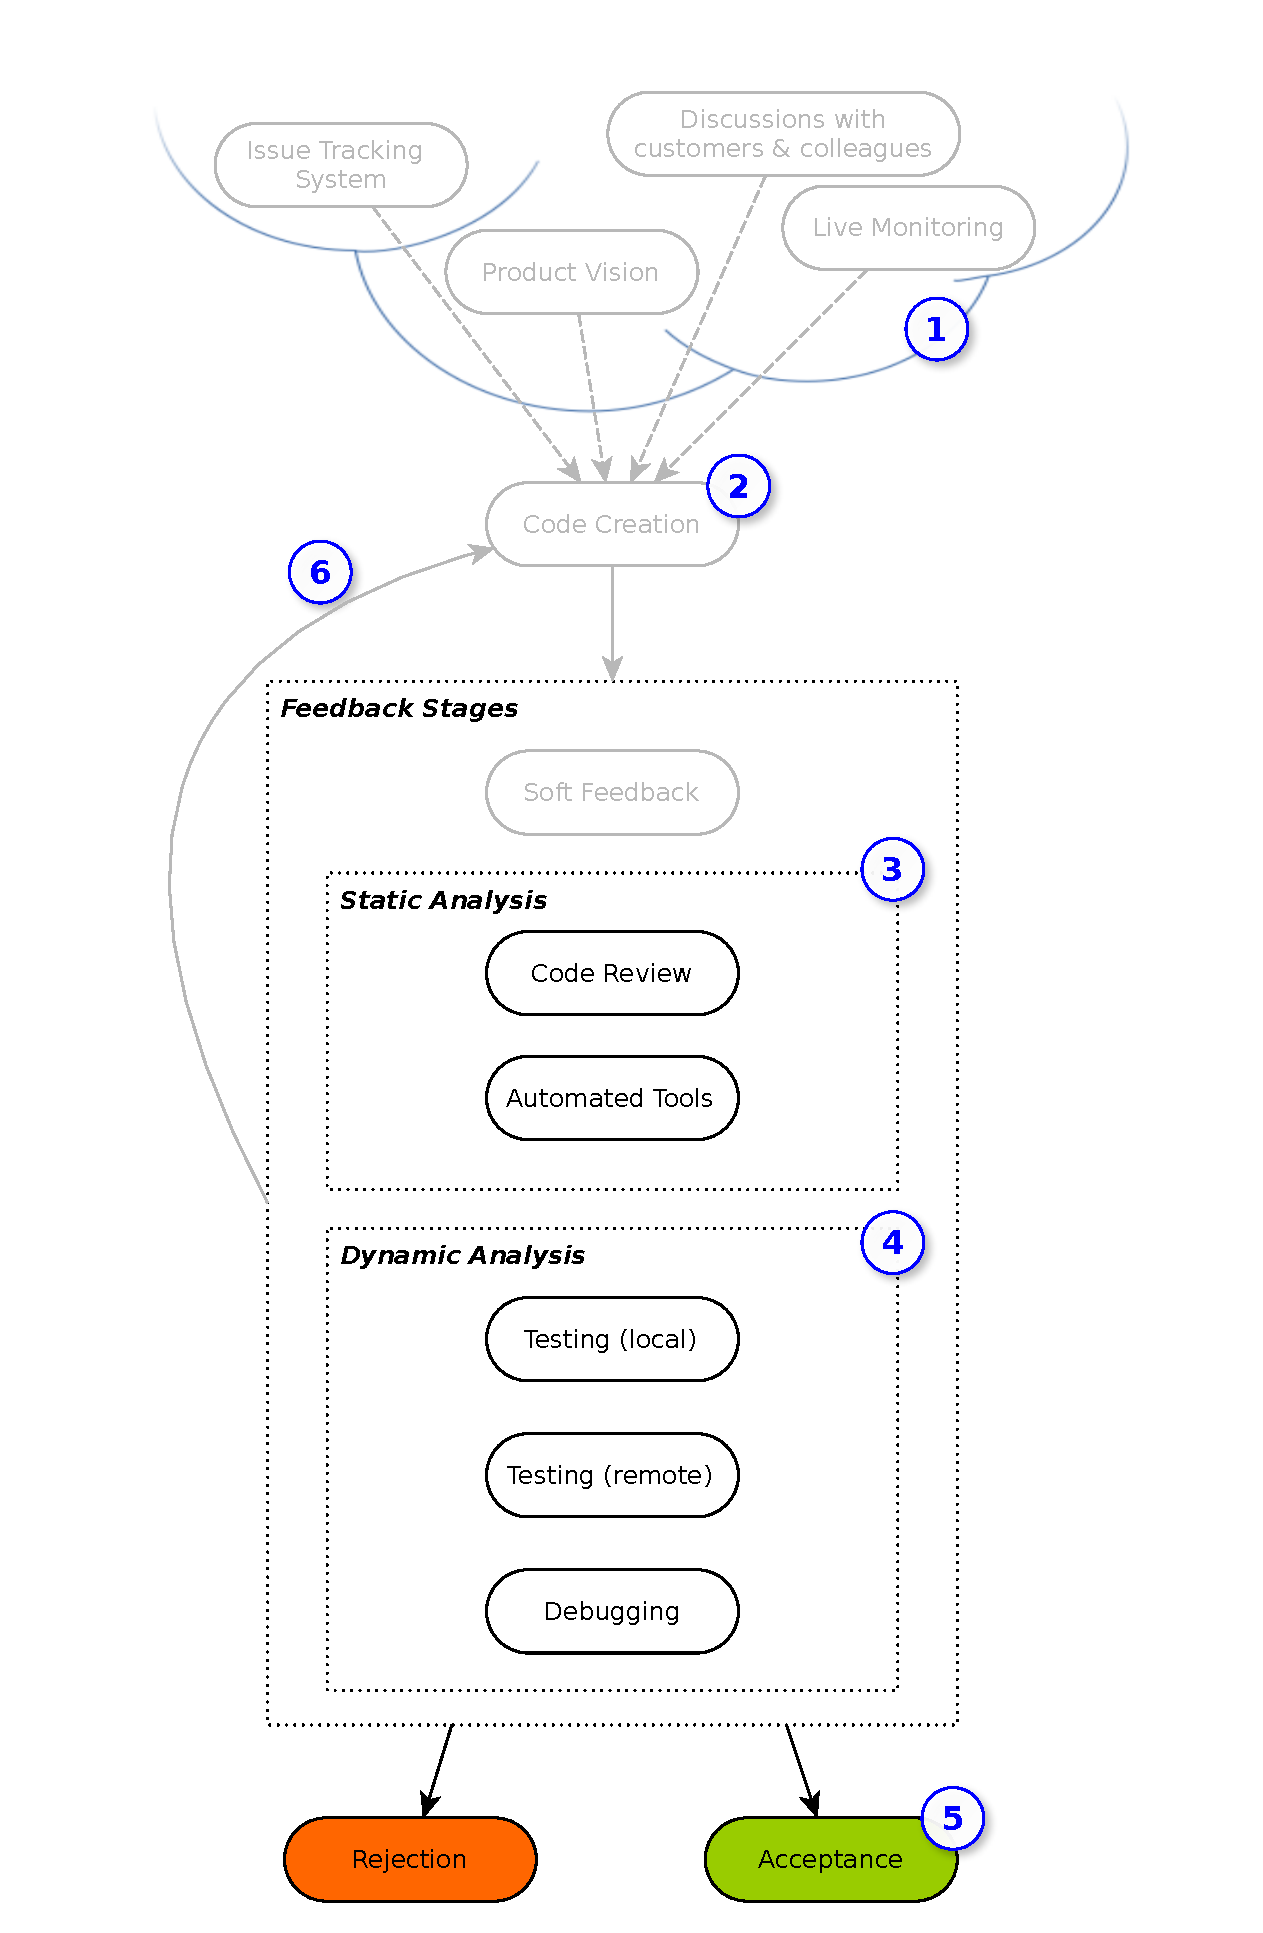
\includegraphics[width=0.65\columnwidth]{development_model_without_papers}
	\caption{The stages of the FDD model and their relationship to other
          Software Engineering concepts.}
	\label{fig:devmodel}
\end{figure}

We also have lists:

\begin{enumerate}
  \item Static Analysis~\circled{3} examines program artifacts or
    their source code without executing them~\cite{wichmann1995industrial}, while
 \item Dynamic Analysis~\circled{4} relies on information gathered from their
   execution~\cite{cornelissen2009systematic}.
\end{enumerate}

Or boxes:

\begin{framed}
This thesis is concerned with the empirical assessment of the state of the art of how developers
drive software development with the help of feedback loops.
\end{framed}

Or code:
\begin{lstlisting}[caption={\textsc{TrinityCore}},label={lst:e1}]
 x += other.x;
 y += other.y;
 z += other.y;
\end{lstlisting}


I hope this helps you get started!
Moritz

\end{refsection}
\part{Federated learning in healthcare }

\begin{refsection}
\chapter{Multi-central healthcare ecosystems}

\label{Bookchapter}

\begin{abstract}
\dropcap{W}ith recent developments in medical imaging facilities, extensive medical imaging data is produced every day. This increasing amount of data provides an opportunity for researchers to develop data-driven methods and deliver better healthcare. However, data-driven models require a large amount of data to be adequately trained. Furthermore, there is always a limited amount of data available in each data center. Hence, deep learning models trained on local data centers might not reach their total performance capacity.
One solution could be to accumulate all data from different centers into one center. However, data privacy regulations do not allow medical institutions easily combine their data and this becomes increasingly difficult when institutions from multiple countries are involved. Another solution is to use privacy-preserving algorithms, which can make use of all the data available in multiple centers while keeping the sensitive data private. Federated learning (FL) is such a mechanism that enables deploying large-scale machine learning models trained on different data centers without sharing sensitive data. In FL, instead of transferring data, a general model is trained on local datasets and transferred between data centers. FL has been identified as a promising field of research, with extensive possible uses in medical research and practice. This paper introduces FL, with a comprehensive look into its concepts and recent research trends in medical imaging.


\end{abstract}

\blfootnote{This chapter is partly based on \faFileTextO~\emph{E. Darzidehkalani et al. Federated learning in
medical imaging
Part (I): towards
multi-central healthcare
ecosystems, and E. Darzidehkalani. Federated learning in
medical imaging
Part (II): methods, challenges and considerations}.
}


\newpage

% \dropcap{T}his is a introductory page.



% keywords can be removed
% \keywords{Federated learning \and Privacy-preserving machine learning \and  Medical imaging}


\section{Introduction}

\dropcap{D}eep learning has shown great promise in the field of radiology. It has been used extensively in various medical imaging domains and has already helped clinicians and radiologists in numerous ways. The area of radiology has dramatically benefited from deep learning research. It has been shown that deep learning can improve the existing models of tumor detection, from early processing stages such as image enhancement in Magnetic Resonance Imaging (MRI) and Computed Tomography (CT), noise reduction, lesion detection, and segmentation, disease monitoring. All of these areas have shown great promise for the use of artificial intelligence in clinical settings. 

 Deep neural networks are made up of many layers with billions of parameters, and they train to learn a complex, high-dimensional mapping from raw input data to desired labels.\cite{erfani2016high} The main issue with training deep neural networks in real-world medical practice is that a massive amount of diverse data is needed. A neural network trained on a single dataset from a single institute may be easily overfitted, resulting in a strong bias towards that institute and poor generalization. Furthermore, latent patterns in one client's imaging data may influence the performance of a neural network in ways that have nothing to do with the actual biological way in the image. For example, datasets containing only one modality or images registered on a specific atlas may bias deep learning models towards that modality or atlas, capturing irrelevant data as significant predictors. The quality of data of a single institution depends on a variety of factors such as the number of patients, type or number of imaging machines available,  and the number of experts available at that institution. Not all healthcare facilities have vast amounts of diverse imaging data, and deep learning models are thus usually trained on limited datasets. This makes clinical decision-making burdensome given the low number of cases, which happens more often in rare diseases. \newline One potential solution to this data shortage is to obtain imaging datasets from different clients. This method has the potential to increase both the amount and diversity of data collected. The most frequent method for establishing such a  collaboration is to centralize vast and diverse datasets from multiple institutions and train a deep neural network on an accumulated dataset situated in a central hub, as can be seen in Figure \ref{fig:CDS}. However, this technique is fraught with difficulties; strict national or regional privacy rules, such as GDPR in Europe or HIPAA in the United States, preclude institutions from easily sharing their patients' data. Other impediments may arise due to the multiple stakeholders, including hospitals, patients, researchers, medical physicians, and industrial corporations, each pursuing their interests. The significant amount of time and effort (and hence money) that an institution spends to collect and clean data makes it hesitant to share it with other institutions.
% Another application is for patients with a rare disease. It is often impossible for a single institution or even multiple institutions to reach a consensus about diagnosis, treatment, ...etc of a rare disease given a low number of cases. 

\begin{figure}[h!]
 \centering
  
\includegraphics[scale=0.31]{Centrlizied algorithm.jpg}
  \caption{Centralized data sharing (CDS)}
  \label{fig:CDS}
\end{figure}

Recent advancements in privacy-preserving AI algorithms play an essential role in solving this. They enable researchers and institutions to train their networks on diverse imaging data from multiple institutions while ensuring that data will be kept locally, thus avoiding many issues concerned with building and maintaining an extensive central database. A general methodology in deep learning is decentralized or distributed learning. Distributed learning can be defined as a group of algorithms in which multiple clients do part of the computation or data storage tasks. The data distribution allows numerous clients to participate in the learning process and enables higher performance with a larger input data size. It generally involves multiple nodes and clients doing partial computation, each on then own local database. Distributed learning is done for a variety of reasons, including performance boost and large-scale computation. Federated learning is a version of distributed learning tailored for tasks where data privacy is essential so that researchers can preserve privacy while performing distributed learning. This feature enables healthcare centers to train deep learning models without compromising the privacy of their local data. 


\section{Federated learning algorithms}
\label{sec:FL algorithms}


A deep learning model is a form of algorithm based on artificial neural networks. It utilizes high volumes of data to extract patterns from them. Artificial neural networks generally consist of millions of parameters called model weights. Training a model is the process of tuning the parameters of the neural network to perform a task ( e.g., detection, classification, or segmentation in the imaging domain). The training process is done by exposing the model to a specific dataset for several rounds. 
More rounds and more extensive training data generally lead to more accurate parameter tuning and better model performance.  Generally, models size depends on their complexity and the number of parameters they have, regardless of how much data they were trained on. Popular deep learning models have a size of no more than around 150 megabytes \cite{canziani2016analysis}.

As a result, complex patterns of enormous imaging datasets can be encoded in models with much smaller sizes. One immediate advantage coming from this feature is in distributed settings. Sharing models in these situations would be much more practical than sharing data. Sharing models are thus subject of interest in distributed settings involving voluminous data, e.g., high-resolution images or multi-slice MRI and CT scans.  \\

Federated learning is a distributed learning method in which multiple participants train (or update) a local model on their data without actually sending data to the central node. A global model is updated according to the updated models received from participants. This way of training allows researchers to ensure the privacy of models and distributes the heavy computing process. FL is also efficient in communication since generally, only model weights will be communicated in this setting. In this regard, it tackles the infrastructural barriers of moving large volumes of data from one institution to another. Various ways to harmonize global and local model updates result in multiple versions of FL. Generally, federated networks require multiple clients who hold the data and perform the local training and a central trusted server, which manages the whole process. \\
% \hl{(Can you elaborate on this. Not every physician/radiologist knows what is model weight and why is it smaller) What gets deleted apart from patients identifier? Do you change the image format? How does this affect image resolution? Can you still PACS system to see the images? How about high resolution mammograms with microcalcifications?.}

\begin{figure}[h!]
 \centering
  
\includegraphics[scale=0.17]{figs/training ga.jpg}
  \caption{Communication between client and server, exchanging the model}
 \label{fig:train1}
\end{figure}


Each client trains a model it gets from the central server on its local data. To get the model, the client sends a request to the cloud server, informing that it's ready to start the local training session. Then the request is processed, and the latest global model is sent back to the client. Next,  the training session starts using the received model and local data. After the local training session is finished,
the model is returned and the center accumulates the received updates. Finally, the global model is updated by the server based on the received model and notifies the client that one training round is successfully completed.  A schema of these steps can be found in the Fig. \ref{fig:train1}.  It is important to note that the model used for training in the hospital has to be the same type as the model being used by the central server. For example, both have to use the format in the same programming language. So practically, any form of transfer that preserves the type and information of the local model can be used. There is no certain requirement for communication technology. The information can be delivered using any form of file transmission (e.g., FTP, SFTP, HTTP, and HTTPS) or third-party software using those protocols. There are several python-based packages designed for transferring models in federated settings.\cite{he2020fedml}.  Python environments like Jupyter notebook are preferred to run this software. However, some models support other platforms such as Web-based applications, Android/iOS, and RaspBerry-Pi.\cite{beutel2020flower}




% There exist several FL algorithms, and this paper discusses the most important of them.  McMahan et al. \cite{mcmahan2017communication} proposed a federated averaging method (FedAvG) to minimize parameter change. The algorithm is straightforward: a subset of the clients is selected each round. Training is distributed among multiple clients. Each client will compute an updated model on their own local dataset. All model instances on the clients should start with the same random initialization to achieve convergence. Clients communicate with the central server once their local training has been finished. Finally, the central server gathers the updates of the respective clients. An immediate effect of local training can be seen at this stage. The updated global model can be tested against a test dataset, and comparing its performance with the previous round can give insight into how much improvement was achieved during the last round of training. An illustration of this step is shown in Fig. \ref{fig:train2} Blockchain-based technologies can also be used in the aggregation stage. In a blockchain network, local clients (miners) replace the central server and distribute the aggregation process among themselves. In this case, the whole process will be decentralized. Blockchain networks can be valuable since they prevent failure if the central server or clients fail. \cite{wang2021blockchain} 


% \begin{figure}[h!]
%  \centering
%   
\includegraphics[scale=0.25]{Training step 2.jpg}
%   \caption{Cloud server gathers the locally updated model from clients }
%     \label{fig:train2}
% \end{figure}
 
 
 For a hospital to join a federated learning network, a collaboration between different experts from various areas might be needed. An institutional review board or ethical committee determines how a hospital participates in a federated network and the level of trust to other involved parties. This committee usually suggests the steps to prepare data so that the hospital can connect to other hospitals. PACS managers and hospital technologists access, prepare, standardized and de-identify data according to the guidelines prepared by the review board. Data standardization generally follow the FAIR principles. The FAIR principle consists of Findable, Accessible, Interoperable, and Reusable data collection\cite{wilkinson2016fair}. FL algorithms that could not use the data from various sites due to the difference in the data type could easily read and analyze data collected in the FAIR manner, which helps add more clients to the network.One example is language protocol differences in sites. Uniform Resource Identifier (URI) could represent the clinical data, enabling automated algorithms to read clinical text queries standardized with FAIR principles\cite{masinter2005uniform}. Integrating FAIR data collection and adding it as an initial step of building an FL network could strengthen the FL networks and ease more institutions to join the networks.
 The FAIRified data will be then given to data scientists and machine learning engineers to build an FL framework.  Clinicians participate by providing annotated data and expert support. They can also take part in assessing models and provide expert feedback. 
% \begin{figure}[h!]
% \centering
%   
\includegraphics[scale=0.25]{federated averaging.jpg}
%   \label{fig:train2}
%   \caption{FedAvg}
% \end{figure}
% Another approach is averaging the outputs of the local models trained on the clients individually (ensemble single client models).A general definition for ensemble learning is different machine learning algorithms doing the same task are combined into one algorithm. Each algorithm extracts information or features from the input data, and the resulting information will be fused using various mechanisms, such as averaging, and voting. Generally, ensembles consistently outperform each of their consituting algorithms alone. In the federated setting of ensemble learning,  neither the models nor the data will be shared among clients in the training cycle. All the clients will be assigned a similar model with random initial values. Each client will train its model. Their outputs for the same task will be averaged in the deployment phase, resulting in an accumulated knowledge from multiple models.  


% \begin{figure}[h!]
% \centering
%   
\includegraphics[scale=0.3]{Ensemble methods.jpg}
%   \label{fig:train2}
%   \caption{Ensemble models}
% \end{figure}





% \begin{figure}
%      \centering
%      \begin{subfigure}[b]{0.43\textwidth}
%          \centering
%          
\includegraphics[scale=0.32]{Ensemble methods.jpg}
%          \caption{}
%          \label{fig:y equals x}
%      \end{subfigure}
%      \hfill
%      \begin{subfigure}[b]{0.43\textwidth}
%          \centering
%          
\includegraphics[scale=0.27]{federated averaging.jpg}
%          \caption{}
%          \label{fig:three sin x}
%      \end{subfigure}
%      \\ [10pt]
%      \centering
%     %  \hfill
%      \begin{subfigure}[b]{0.41\textwidth}
%          \centering
%          \raisebox{\dimexpr\ht\imagebox-\height}{ \includegraphics[scale=0.3]{SWT algorithm.jpg}}
        
%          \caption{}
%          \label{fig:five over x}
%      \end{subfigure}
%     %  \hspace{0.2\textwidth}
%      \hfill
%      \begin{subfigure}[b]{0.41\textwidth}
%          \centering
%         %  \hfill
%          
\includegraphics[scale=0.3]{CWT algorithm.jpg}
%          \caption{}
%          \label{fig:five over x}
%      \end{subfigure}
%         \centering
%         \captionsetup{justification=centering}
%         \caption{Schema of different decentralized learning methods, (a) Ensemble methods, clients train local models on their own dataset,model outputs of different clients are averaged. (b) FedAvg, an initial model is sent to the clients, each train the model on their own data and the resulting local models are averaged in a central server. (c) SWT, an initial model is sequentially passed through clients and visit each clients once. Final model is the model trained on the latest client. (d) CWT, similar to SWT, however, model is passed through institutions multiple times.}
%         \label{fig:three graphs}
% \end{figure}




% A third algorithm is single weight transfer (SWT). In this algorithm, a deep learning model is trained at a single client up to a particular time and then transferred to the next client. There are numerous options to decide when to finish a local training and pass its model to the next client.  Standard criteria are the number of epochs per client and validation loss or accuracy depending on the problem. For example,  Chang et al. \cite{chang2018distributed} chose to reach the plateau of validation loss as a sign of moving to the next client.  Cyclic weight transfer (CWT) is another algorithm in which a model is trained at each client for a predetermined number of epochs, then transferred to the next client. In this algorithm, the model visits each client than once. 

% The functionality of models and tasks in an FL scenario differs depending on the FL algorithm. Algorithms that transfer models are more versatile and adaptable than other algorithms. Deep learning models' performance in a federated environment can also vary from model to model. Models' adaptability can determine the overall performance of an FL network. For example, research has shown that some deep neural network components (such as batch normalization layers) cause performance issues and are harder to adjust in a federated setup. On the other hand, components like convolutional layers could be easily averaged, averaging their results in a proper global model.  As a result, deep learning models that have more suitable components are a better choice for FL. Reseach is going on to develop specific models that perform better in a federated environment\cite{li2021fedbn}.



% \begin{figure}[h!]
%  \centering

%   
\includegraphics[scale=0.25]{Training step 2.jpg}
%   \label{fig:train2}
%   \caption{Communication between client and server, exchanging the model}
% \end{figure}










% \begin{figure}[h]
% \begin{subfigure}{0.25\textwidth}
% \includegraphics[scale=0.25]{SWT algorithm.jpg}
% \label{fig:train2}
% \caption{SWT algorithm}
% \end{subfigure}
% \begin{subfigure}{0.25\textwidth}
% 
\includegraphics[scale=0.25]{CWT algorithm.jpg}
% \label{fig:train2}
% \caption{CWT algorithm}
% \end{subfigure}
% \end{figure}


% \begin{figure}[h!]

%   
\includegraphics[scale=0.25,center]{CWT algorithm.jpg}
%   \label{fig:train2}
%   \caption{CWT algorithm}
% \end{figure}

% \subsection{Comparison of the federated learning algorithms}
% We may categorize the algorithms based on what is exchanged between the server and the client to compare federated algorithms. Techniques such as FedAVG, SWT, and CWT, transfer the model between the server and the clients. Approaches like split learning \cite{poirot2019split}  transfer middle layer outputs of a neural network. The middle layer outputs can be regarded as a distorted form of the input data. In other words, as the neural network processes the input data, it undergoes numerous modifications that distort the input. Methods such as ensemble methods share their models' final output and broadcast it to a central server. 

% The amount of data transferred is relatively tiny in methods in which the model is moved to the central server and is independent of the amount of training data at each site. It is solely determined by the size of the deep learning model. The majority of popular deep learning algorithms are tens of megabytes in size. However, an FL algorithm that transfers a model does not necessarily mean that the overall communication overhead is low. The overall amount of exchanged data also depends on the number of communication rounds between clients and servers. The hyperparameters can determine the number of communication rounds, and communication overhead could be high if there is too much exchange between clients.





% \begin{table}
% 	\caption{Comparison of FL methods}
% 	\centering
%     \resizebox{1.04\textwidth}{!}{
% 	\begin{tabular}{|P{0.07\linewidth} | G{0.13\linewidth}|P{0.06\linewidth} |P{0.1\linewidth}|G{0.10\linewidth} |G{0.13\linewidth}|G{0.13\linewidth} |} \hline
% 		 Methods & Summary & Transferred data & Communication load & Advantages &	Disadvantages &	Usecases\\ \hline
% 		FedAvg$^{*}$ & In each round, every client trains the global model on local data. Then models are averaged &Model &	low	&Easily converged&Weak robustness  with imbalanced clients distribution&COVID-19 CT scans \cite{dou2021federated} \newline
% 		Lung nodule detection  \cite{baheti2020federated} 
%  \\ \hline
%  SWT$^{**}$ &
% 		model is passed through clients sequentially, visits each client once	&Model&	Very low&	Low communication load&	Highly biased towards the latest institution &	Diabetic retinotherapy  \cite{chang2018distributed},\newline Mammography  \cite{chang2018distributed}

%       \\ \hline
% 	CWT $\dagger$ &	Model is passed through clients sequentially; the sequence is repeated multiple times&Model&low&High performance&	Needs many rounds to converge&Breast cancer data\cite{beaulieu2018privacy} EHR \cite{beaulieu2018privacy}

%   \\ \hline
% 		Ensemble methods&All the computations are done locally the outputs are averaged&Output&High&Easy to deploy&	High possibility of data leakage, High communication load&Patient health records \cite{li2016distributed} 

%  \\ \hline
% 		CDS$^{\ddagger}$&Move data from clients into a central datacenter&Data&-&High performance&No privacy&MR image reconstruction \cite{Quan2018compressed} , dermoscopy image synthesis \cite{DBLP:journals/corr/abs-1804-03700}
%   \\ \hline
%   \multicolumn{4}{l}{\tiny *Federated averaging **Single weight transfer    ${\dagger}$Cyclic weight transfer   $\ddagger$ Centralized data sharing } \\
% 	\end{tabular}}
% 	\label{tab:table}
% \end{table}
% % \footnotesize{$^a$ The smallest spatial unit is county, $^b$ more details in appendix A}\\


% % (Add the abbreviations with table legend at the bottom of the table)
% On the other hand, in algorithms that transfer some type of actual data, whether distorted input data  (e.g., split learning \cite{poirot2019split}) or output data (e.g., ensemble models), the size of sent data can vary greatly depending on the data size. However, because medical imaging data is enormous, the amount of communicated information is usually more significant than with methods that transfer the model. CDS also falls into this category, as it requires actual data transfer to a central server. These two groups differ significantly in terms of communication burden as well as privacy level. Because input/output data is not sent in any format, methods which transfer models are more secure since retrieving patient data from deep learning models is difficult.

% In Ensemble models, the ensembling process is done locally, and outputs of the models are sent to the global server instead of model parameters. As a result, heavy server-side computations are avoided and a federated network can be set up easily. Since ensemble models are proven to perform well in various areas of medical imaging, using ensembles can help improve the accuracy, generalizability, and stability of a federated network.

% However, ensemble methods impose some challenges. First, the risk of data leakage is serious in this setting. Some sort of output data like segmentation masks is very likely to reveal patients' identities. Second, contrary to model size, outputs can vary quite a lot in their size. Outputs in image format require too much communication load. 
% In addition, ensemble models are design dependant. Models that do not necessarily share the same objective function can be combined into one ensemble. This leads to one complex multi-objective model having disparate optimization goals. This is not necessarily harmful, but there is a lack of research on the theoretical analysis of ensembles, and the result of an ensemble remains almost always unclear, making ensemble methods unreliable.

% Besides, there is always a compromise between training time, model complexity, performance and generelizability. Altough these measures have been thoroughly investigated in single machine learning models, the literature on their relationship in a complex ensemble is still not explored much.



% Another aspect of comparing FL models is that FL algorithms, in which a model is transferred, can consistently be averaged by the central server, regardless of the task they are performing. Deep neural networks performing classification, segmentation, regression, or other tasks could be averaged as long as there is a proper deep learning model for that.  All of the mentioned tasks have been demonstrated and proved to work in a federated manner. However, averaging the output from many sources is not always feasible for other federated earning algorithms. For example, if the task is multi-class classification, an ensemble approach cannot simply average the class output of distinct clients. The Ensemble approach is thus limited in the jobs it can tackle.


% Several research papers have been published that compare FL implementations. Nilsson et al. \cite{nilsson2018performance} compared various FL methods in practice. They demonstrated that FedAvg is the best FL algorithm. Despite having slightly lower performance than CDS, it is practically comparable in their comparative performance analysis to a non-federated architecture.
% There are numerous variants of the FedAvg algorithm and other FL approaches. However, the original FedAvg method remains one of the top methods in comparison studies. Chang et al.\cite{chang2018distributed}investigated several FL algorithms in the radiology area. According to this study, FedAvg does not impose any bias compared to other algorithms because it considers all clients equally and does not arrange them in any particular order. As shown in Figure \ref{fig:three graphs}algorithms such as SWT and CWT, clients are placed in a sequence and trained one after the other. As a result of catastrophic forgetting, the model is more representative of the most recent clients it observed and less of the earlier clients\cite{sheller2020federated}. As a result, there is a bias favoring the most recent institution in models with sequential training. Although CWT can mitigate this effect by running the model through institutions multiple times in a cyclic fashion, bias remains. Table \ref{tab:table} shows the essential characteristics of FL algorithms. There is also a sample of use cases of these algorithms in the medical domain.



\section{Applications in radiology}

Although FL still needs to be improved before it can be used on a large scale, it has shown promise in a practical medical imaging context in a few implementations in medical images, leading to improvements in patient care.  FL can assist underrepresented patients in small clinics where they are a minority and may be overlooked and bring them into a pool with many other similar patients. FL has shown great promise in the research for COVID-19 patients; it was investigated and reported that FL had a clear impact on patient care in a large-scale study on COVID-19 patients across 20 centers on five continents\cite{flores2021federated}. They used chest X-Ray imaging data in addition to clinical data to determine hospital triage for level of care and oxygen requirement in COVID-19 patients. They demonstrated that the FL model works best for clients with limited datasets. The model performance for these clients is significantly improved compared to when they were trained on their local data, resulting in a change in the patient situation. 

Another discovery was that medical centers with unbalanced data had some classes with few samples, resulting in underrepresented categories. These clients saw a significant improvement in prediction for those patient categories, which is especially important because, in COVID-19, patients with severe symptoms are generally in categories with fewer samples than a larger pool of patients with moderate symptoms. However, their care is more critical and requires more attention.  In the field of applied FL in radiology, there are numerous projects. As an additional effort to the BraTs challenge, Intel and the University of Pennsylvania launched an extensive effort. This challenge was based on a dataset provided by the University of Pennsylvania's Biomedical Image Analysis section (SBIA)\cite{bakas2017advancing}.  

The Brain Tumor Segmentation dataset from the 2018 BraTs challenge was made available to the public. The dataset consisted of MRI images of glioma patient's brains,  gathered from several studies in different institutions. Four radiologists manually annotated the MRI images, categorizing them into various Tumor classes. Tumors were classified into four types. U-Net was the deep learning model used to segment tumors, and the FL network was made up of one master node and numerous clients, each with their data. Two hypothetical clients were developed, and the dataset was assigned to them to evaluate the FL model. To examine different data distribution algorithms, they first divided the data randomly into silos. They also assigned data based on where it was obtained, resulting in non-homogeneous data. After finishing the local training, many clients delivered a model. The central server received updated models from all parties, selected the best models, and returned the aggregated models to the clients. This training strategy allows both the server and the clients to enhance their performance. After receiving the updated model from the central node, clients work on a better model each round. As a result of their experiments, they concluded that in the task of semantic segmentation, federated training could produce MRI segmentation masks that were better or comparable to models trained on-premise. 


% Another study, a partnership between King's College London and Nvidia corporations, published at the MICCAI 2019 conference, also used the BraTS dataset. \cite{lee2018privacy} They employed a noise-adding strategy to improve medical record security across many data centers. The data was encrypted before being delivered to the central node in the approach they presented; they also anticipated reverse engineering methods could reveal the actual patient data. Therefore, they took intricate mathematical precautions into account. Nvidia was again able to get results comparable to a CDS setting while protecting patients' personal information. 
Sheller et al.\cite{sheller2020federated}proposed a project on brain tumor segmentation using FL and achieved comparable accuracy to CDS. They demonstrated that increasing the number of collaborators improved the FL algorithm's performance and generalizability. Another study suggested a patient similarity analysis to find comparable patterns within different hospitals for possible similar treatments\cite{lee2018privacy}.
% (This is not radiology related, I guess you can still have it in the paper)
The goal of this study was the identification of patients with similar profile while protecting their privacy and personal information. They created hash codes to represent patients and a federated environment to control the entire process to achieve this goal. The hashed data had the advantage of being resistant to reverse engineering or adversarial model attacks. They could anticipate five diseases independently, using balanced and unbalanced data to evaluate their proposed algorithm. 

% Pan et al., \cite{pan2019improving} investigated the impact of the model ensemble for automatic bone age estimation based on imaging data. The results showed that combining heterogenous, uncorrelated models leads to more robust ensembles. Conversely, naively combining top models does not necessarily ensure top-notch performance.
% They were able to demonstrate how data FL can aid in identifying comparable patients while protecting their privacy. 
Another effort was made to explore the structural relationship of the brain without revealing any data. The authors used Principal component analysis (PCA) to uncover anatomical relationships between diverse datasets in a federated setup\cite{grammenos2019federated}. Federated PCA could extract features from MRI pictures from several medical institutes. Their technique was validated using several databases, including ADNI, PPMI, MIRIAD, and UK Biobank\cite{silva2019federated}.

Balanchandar et al. \cite{balachandar2020accounting} using FL to address the issue of data variability across institutions. They used chest-Xray dataset to classify chest scans. Also, they classified retinotherapy data with their proposed method.




% \section{Challenges and considerations}
% \label{sec:others}

% FL still has a long way to go in radiology. There are numerous challenges both in the theoretical formulation and practical implementation. FL algorithms could be divided into fully decentralized/peer-to-peer methods requiring a trusted central server. Each category comes up with its challenges. Generally speaking, methods with a central server offer more flexibility and better performance, while decentralized methods are more reliable and secure.

% However, there is still some risk associated with the FL infrastructure \cite{yin2021see}. An adversary could reconstruct private data from the local model updates\cite{wang2019beyond}. Hospitals can do additional security measures to prevent adversaries from accessing the exchanged data between the server and clients.



% \subsection{Data heterogeneity }


% The FedAvg algorithm authors claim that their proposed method can handle heterogeneous data. However, the decentralized structure of the data makes data processing challenging to verify the completeness and quality of their findings. Further investigations revealed that this claim is not always valid\cite{li2020federated}. In almost all cases, heterogenous data deteriorates the accuracy of the FL model. The degree of divergence depends on how heterogenous the data is. Local models are trained on data with different patient profiles, resulting in a global model that could not represent all of the profiles. In some cases, heterogenous data prevents model convergence.    


% Data homogeneity significantly impacts the version of the federated model to be chosen to train the model. The difference between CDS and FL might vary from similar to CDS better depending on the data. One rule of thumb would be that if data has very different distribution in different data centers, simply averaging each client's data in every round might affect the performance negatively.



% Zhao et al.\cite{zhao2018federated}examined the effect of bias that distributing data can have on final performance of FL algorithms. According to their study, difference in data distribution can have negative effect on the model accuracy up to 55\%. Another difficulty is that data heterogeneity might lead to a situation where a best global model might be a poor model for some clients, or a best global model might work quite well on some clients and perform poorly on other clients. Consequently, all participants should agree on the concept of optimum model training in advance of the training. Further technical studies should be carried out to find the optimum technique for updating the central model with heterogeneous data. FedAvg is the standard method for accumulating the data from clients. Still, other distributed optimization methods that can tackle distribution differences are a subject of research.



% \subsection{Bias}
% Bias is a prevalent issue in distributed networks. Bias is a state that a neural network is inclined towards the distribution of a client more than other clients. It results in the model performing well on that client by compromising the performance on the other clients. The cause of bias could be the difference in the size or the distribution of clients' data. Also, the FL algorithm itself could be a source of bias.


% Sheller et al.\cite{sheller2020federated}showed that CWT is a less biased algorithm than SWT. The degree of bias could vary, depending on which client was trained last.They favored FedAvg over SWT and CWT. FedAvg did the FL more fairly.  There is always a bias toward the latest clients they were trained on for algorithms like SWT and CWT. In FedAVG, however, the results of local training are aggregated every round, avoiding bias. In SWT, the global model changes after visiting each client, and succeeding clients mitigate the model's bias towards the preceding institutions. However, there is no mitigation for the latest institution the model is trained on.





% The global aggregation method, i.e., server algorithm, should be designed to minimize bias . It also should be robust to local variations, as well as perturbations added by security measures. Reducing bias and designing models that capture diversity is possible by calculating the level of bias arising from each client. Then modifying the  algorithm to address the difference in the distributions. 


% However, if the distribution difference is taken into account properly, bias might still emerge later in training. Some features, as well as general data distribution might vary over time.  For example, the number of patients with a particular disease in a particular hospital might change for several reasons. This can cause a domain shift: a change in a client's data distribution. There could be more work on data domain shifts and somehow explicitly address the alterations in gender, patient profile, age, and disease among different institutes or one institute. Models could also be further developed to consider economic or racial status into model training and modify a model to handle diversity in images\cite{li2020multi}. 


% \subsection{Lack of standard data}
% Standardizing data prevents irrelevant information from being considered meaningful in neural networks. It removes the variability between institutions.  Electronic data management is the norm in medical imaging: and medical communications (DICOM) is the globally recognized image data format and the near-global care standard for electronic file storage. However, not all the available data in the medical imaging sector is standardized. Many institutions still lack the infrastructure to handle their imaging data according to current management standards. 
% One factor is the lack of a universal method to organize and manage patient records. Data management is expensive\cite{wang2003cost}. Not all hospitals have advanced data management facilities. This issue leads to the preselection of hospitals participating in research, which is a source of bias.  



% Medical data are very diverse because of the diversity of modalities, dimensionalities, and features and because of variables such as variances in the acquisition, medical equipment brand, or local demographics within a specific protocol. There is still no uniform data standardization method. As a result, healthcare federated networks are likely to have clients with disparate data quality and distribution. Methods like FedAvg are generally likely to fail under these circumstances.  One way to avoid bias is to harmonize data and make each client data type similar, following a similar preprocessing. This also might require sharing metadata among institutions to find a general method of harmonization in data that suits all the institutions. But this could be tricky given the restrictions of individual institutions. Hence, one way of further development for FL systems is that the clinicians and computer scientists collaborate to standardize handling data among multiple institutions concerning the privacy restrictions and considerations.



% \subsection{Privacy and Security}
% Data breach is a major concern and medical data and must be safeguarded in compliance with accepted confidentiality procedures. FL has proven to be effective in protecting patients' privacy and anonymity by keeping data locally. However, there are some privacy-related challenges associated with FL. Despite many attempts to de-identify personal data from DICOM images, patient information could still be re-identified\cite{Peter2015Free} \cite{monteiro2015machine}. Recent studies have successfully rebuilt a patient's face from their MRI data. Furthermore, adversaries could steal the data or access the algorithm for non-encrypted networks. 


% Furthermore, deep learning models still have some sensitive information in the weights they carry. On a decentralized network, it is feasible to reconstitute portions of patients' information only having the local model from one client\cite{carlini2019secret} \cite{zhang2020secret}
% \cite{hitaj2017deep}. Adversaries can decrypt deep learning models and reveal patients' information with a very high accuracy\cite{fredrikson2015model}. Malicious parties can distort the deep learning models. False outputs produced by such models can have severe consequences if used in practice. As a result, it should be ensured that models are secure and that adversaries cannot breach models to be employed in the real-world setting\cite{tomsett2019model}.



% There are specific measures to improve privacy. Particular countermeasures, such as model encryptions, Differential privacy (DP), \cite{abadi2016deep} adversarial defense against malicious clients,\cite{hitaj2017deep} and increased communication security, can be done. DP refers to the practice of keeping a dataset's global statistical distribution while minimizing individually identifiable information. DP can be done by adding perturbation to each sample.Adding noise to a dataset to reduce the chance of private data being revealed is based on the argument that one can preserve general data distribution while individual samples are changed by randomly altering a dataset. Adding systematic noise helps machine models to learn the whole distribution of training data while keeping each sample anonymous.


% However, such countermeasures complicate the training algorithms and can affect training performance. Sometimes much longer training times are required, or accuracy will be dramatically decreased. This can impose an additional cost on the whole network. Hence, it is quintessential to consider whether deploying a countermeasure is necessary. The cost-efficiency of implementing them depends mainly on the level of trust among involved parties and the project scale. If clients do not trust each other, then DP is a necessity. This is because federated clients have regular communication, and critical information can be exchanged in the interactions. So each client's data should be safeguarded from other clients. This shows how important it is to clarify the level of trust among clients. This argument holds true in fully decentralized algorithms, where no central node is involved. And also in algorithms including a central server, where the client/server trust is also essential. 
% Total image anonymization is still a problem. In the absence of encryption, attackers may acquire private information from local datacenters or intercept the communication pathways and rob the passing data.


% \subsection{System architecture}

% Medical data in federated networks requires on-premise or cloud-based data storage. Hospitals might need private or cloud-based computing power. As well as software for preprocessing and standardization of data, such as PACS. To allow the local model training hardware (GPU), connections and data centers should be set up in local centers. These bring their challenges, such as high computational power to assure harmony with other clients and high-performance bandwidth and connection between different centers, which is not always feasible in medical centers. Many hospitals still lack computing resources and strong internet connections \cite{li2010securing}. Besides, for the whole network to work correctly, redundant computational facilities and data centers should be devised to prevent data loss. If one computational client fails, the network could continue its training, which imposes an additional challenge. Robustness of the network is also critical ;federated models should be structured so that adding or removing clients and increasing or decreasing the amount of data in a center does not negatively impact patient data or model privacy.




\section{Future of federated learning research}

There are several research trends showing that FL research is growing. The future direction of FL is to integrate it with big data technologies. After establishing FL networks, data could be added to the existing networks in real-time. Allowing the training and inference phase to work in real-time is a potential future direction of FL networks. This can be as streamlining pre-processing, training and, data handling.
\\

It is expected that Federated networks include medical imaging data and work on all other types of medical data. Most of the recent FL implementations make use of imaging data with neural networks specifically designed for image processing. However, other formats of data, especially Electronic health records (EHR), are starting to be added to the current networks and are a contemporary development topic. EHR data are including a wide variety of information from treatment histories to past medication in addition to the medical imaging data EHR data can generally be in text, medical letters, categorical data, quantitative numbers, and binary data\cite{seymour2012electronic}. Incorporating this information into the imaging data could help develop better models. For example, making various treatment plans as an input variable to a deep learning model could help radiologists choose between treatment plans. Using EHR data could also help determine the type/stage of disease, as researchers recently used EHR to detect Alzheimer's disease\cite{venugopalan2021multimodal}.
\\

There is still research to convert EHR data formats to a format usable by deep neural networks. Some progress has already been made using Natural language processing (NLP) to make text records available for deep learning\cite{dreisbach2019systematic}. For this purpose, researchers developed a data standardization framework to extract meaningful features from text data and make them available in the ML pipelines.  Medical images combined with genomics data could also be a line of research. Because genomics data are not as prevalent and readily available as imaging data, the data limit problem in genomics is a much bigger issue than medical imaging. Hence, FL can play a pivotal role in bringing genomics data to the medical imaging field. Medical centers can communicate through FL with all types of their data in the future, so the collaboration level is expected to expand.
\\
% It is also expected that FL can open its way into medical institutions by bringing in more medical experts to the AI field. Trust in AI in healthcare is yet to be established among many clinicians. In 2016, IBM released Watson for Oncology, a technology that searches an extensive database to advise clinicians on therapies\cite{somashekhar2017early}.  Several oncologists claimed they trust their judgment more than Watson's recommendations. Doctors should be included in the training process. They can be involved in data curation and annotation. Because every dataset obtained here cannot be of high quality, it will be advantageous if evidence-based machine standards are created. Doctors will also see artificial intelligence diagnosis criteria. It also helps to make deep learning models work better with more amount of annotated data.


\section{Conclusion}
   Federated learning is a developing and growing technology that has influenced a variety of aspects across several fields. 
The main reason that hospitals are moving towards FL technologies is that privacy and security are their main priorities, and there are strict rules regarding the privacy of patients' data. FL offers straightforward and secure data access for institutions, and utilizes the capacity of several institutions to enhance radiology research while overcoming the limitations of privacy and data sharing laws and regulations. Building a federated environment helps in achieving performance equivalent to a centralized setting. It can foster global cooperation among several institutions, therefore redefining the paradigms of artificial intelligence in radiology. 
This article should be helpful for radiologists and data scientists who want to learn about FL ideas and their applications in radiology. 
% Citations use \verb+natbib+. The documentation may be found at
% \begin{center}
% 	\url{http://mirrors.ctan.org/macros/latex/contrib/natbib/natnotes.pdf}
% \end{center}

% \bibliographystyle{unsrt}
% argument is your BibTeX string definitions and bibliography database(s)
% \bibliography{chapter2}

% Here is an example usage of the two main commands (\verb+citet+ and \verb+citep+): Some people thought a thing \citep{kour2014real, hadash2018estimate} but other people thought something else \citep{kour2014fast}. Many people have speculated that if we knew exactly why \citet{kour2014fast} thought this\dots

% \subsection{Figures}
% \lipsum[10]
% See Figure \ref{fig:fig1}. Here is how you add footnotes. \footnote{Sample of the first footnote.}
% \lipsum[11]

% \begin{figure}
% 	\centering
% 	\fbox{\rule[-.5cm]{4cm}{4cm} \rule[-.5cm]{4cm}{0cm}}
% 	\caption{Sample figure caption.}
% 	\label{fig:fig1}
% \end{figure}

% \subsection{Tables}
% See awesome Table~\ref{tab:table}.

% The documentation for \verb+booktabs+ (`Publication quality tables in LaTeX') is available from:
% \begin{center}
% 	\url{https://www.ctan.org/pkg/booktabs}
% \end{center}


% \begin{table}
% 	\caption{Sample table title}
% 	\centering
% 	\begin{tabular}{lll}
% 		\toprule
% 		\multicolumn{2}{c}{Part}                   \\
% 		\cmidrule(r){1-2}
% 		Name     & Description     & Size ($\mu$m) \\
% 		\midrule
% 		Dendrite & Input terminal  & $\sim$100     \\
% 		Axon     & Output terminal & $\sim$10      \\
% 		Soma     & Cell body       & up to $10^6$  \\
% 		\bottomrule
% 	\end{tabular}
% 	\label{tab:table}
% \end{table}

% \subsection{Lists}
% \begin{itemize}
% 	\item Lorem ipsum dolor sit amet
% 	\item consectetur adipiscing elit.
% 	\item Aliquam dignissim blandit est, in dictum tortor gravida eget. In ac rutrum magna.
% \end{itemize}

% \section{Background \& Context}
% In this thesis, you can reference pictures~\Cref{fig:devmodel} using Cleverref and circles \circled{5}.

% \begin{figure}[htb]
% 	\centering
% 	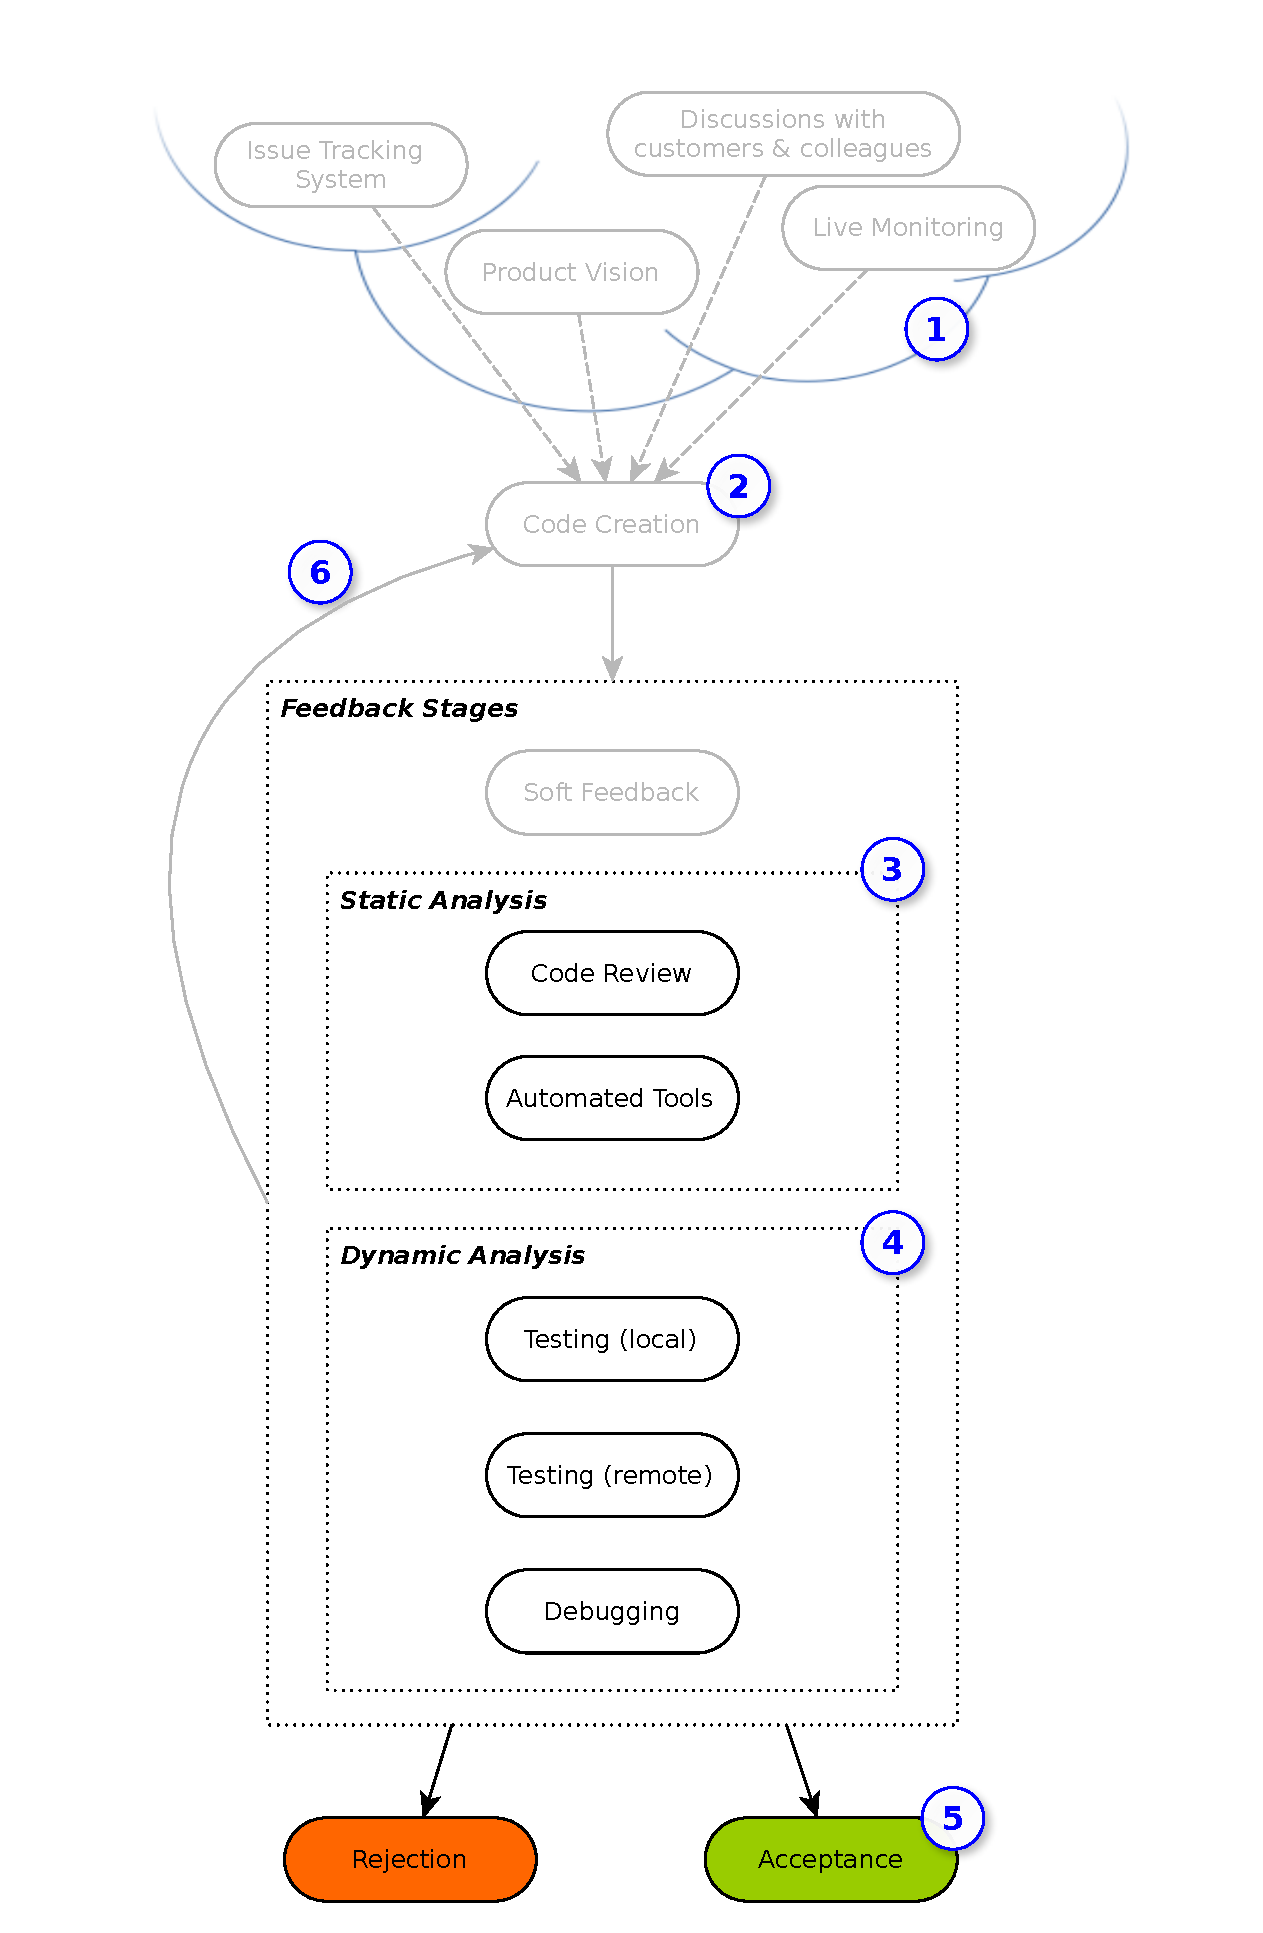
\includegraphics[width=0.65\columnwidth]{development_model_without_papers}
% 	\caption{The stages of the FDD model and their relationship to other
%           Software Engineering concepts.}
% 	\label{fig:devmodel}
% \end{figure}

% We also have lists:

% \begin{enumerate}
%   \item Static Analysis~\circled{3} examines program artifacts or
%     their source code without executing them~\cite{wichmann1995industrial}, while
%  \item Dynamic Analysis~\circled{4} relies on information gathered from their
%   execution~\cite{cornelissen2009systematic}.
% \end{enumerate}

% Or boxes:

% \begin{framed}
% This thesis is concerned with the empirical assessment of the state of the art of how developers
% drive software development with the help of feedback loops.
% \end{framed}

% Or code:
% \begin{lstlisting}[caption={\textsc{TrinityCore}},label={lst:e1}]
%  x += other.x;
%  y += other.y;
%  z += other.y;
% \end{lstlisting}
% \bibliography{Chapter2/chapter2}
% \bibliography{dissertation}
% \printbibliography

% I hope this helps you get started!
% Moritz

% \chapter{Challenges and considerations in Federated learning
% }
% \label{Bookchapter}

% \begin{abstract}
% \dropcap{F}ederated learning is a machine learning method that allows decentralized training of deep neural networks among multiple clients while preserving the privacy of each client's data. Federated learning is instrumental in medical imaging due to the privacy considerations of medical data. Setting up federated networks in hospitals comes with its unique challenges, primarily because medical imaging data and federated learning algorithms each have their own set of distinct characteristics. This article introduces federated learning algorithms in medical imaging and discusses technical challenges and considerations of real-world implementation of them.




% \end{abstract}

% \blfootnote{This chapter is partly based on \faFileTextO~\emph{M. Beller. Toward an
%     Empirical Theory of Feedback-Driven Development, ICSE'18 (Student Res
%     earch Competition)}~\cite{BellerSRC2018}.
% }


% \newpage

% \dropcap{T}his is a introductory page.



% keywords can be removed
% \keywords{Federated learning \and Privacy-preserving machine learning \and  Medical imaging}


\section{Introducing FL methods}

With the rapid developments in machine learning in healthcare and computer-aided diagnosis, access to medical data has become a matter of interest. Clinicians, computer scientist and medical technologists require access to more data to enable machine learning based projects. However, there is always a challenging task to balance between building more powerful machines to be used in healthcare industry, and the limitations of accessing large amount of data under the privacy considerations. Generally, sharing data requires hospitals to deal with GDPR restrictions and have an approval from the institutional review board .An institutional review board or ethical committee determines to which degree a hospital can share information with other hospitals and ensures that the GDPR restrictions are complied to. As a result , datacenters in hospitals do not usually have large and diverse datasets required to train deep neural networks. 

Federated learning (FL) \cite{mcmahan2017communication} 
is a machine learning concept proposed by McMahan et al. to tackle this problem. In this concept, a neural network is trained with datasets from multiple hospitals, and the whole training process is managed through a central server. At each round, hospitals train a neural network on their local data, and share the updated models with the central server. The server gathers all the updated models and aggregates them into an updated global model. In the next round, the updated global model is sent back to the hospitals. This way of training enables the researchers to utilize the data from multiple clients, while ensuring that the sensitive data is kept locally. 


There exist several FL algorithms.McMahan et al. \cite{mcmahan2017communication} proposed federated averaging method (FedAvG) to minimize parameter change among hospitals. The algorithm is straightforward: a subset of the clients is selected each round. Training is distributed among multiple clients. Each client will compute an updated model on their own local dataset. All model instances on the clients should start with the same random initialization to achieve convergence. Clients communicate with the central server once their local training has been finished. Finally, the central server gathers the updates of the respective clients. An immediate effect of local training can be seen at this stage. The updated global model can be tested against a test dataset, and comparing its performance with the previous round can give insight into how much improvement was achieved during the last round of training. An illustration of this step is shown in Fig. \ref{fig:train2} Blockchain-based technologies can also be used in the aggregation stage. In a blockchain network, local clients (miners) replace the central server and distribute the aggregation process among themselves. In this case, the whole process will be decentralized. Blockchain networks can be valuable since they prevent failure if the central server or clients fail.\cite{wang2021blockchain} \newpage 
\begin{figure}[h!]
 \centering
  
\includegraphics[scale=0.22]{Training step 2.jpg}
  \caption{Cloud server gathers the locally updated model from clients }
  \label{fig:train2}
\end{figure}


Another approach is averaging the outputs of the local models trained on the clients individually (ensemble single client models).A general definition for ensemble learning is different machine learning algorithms doing the same task are combined into one algorithm. Each algorithm extracts information or features from the input data, and the resulting information will be fused using various mechanisms, such as averaging, and voting. Generally, ensembles consistently outperform each of their consituting algorithms alone. In the federated setting of ensemble learning,  neither the models nor the data will be shared among clients in the training cycle. All the clients will be assigned a similar model with random initial values. Each client will train its model. Their outputs for the same task will be averaged in the deployment phase, resulting in an accumulated knowledge from multiple models.
\begin{figure}[h!]
 \centering
  
\includegraphics[scale=0.32]{Ensemble methods.jpg}
  \caption{Cloud server gathers the locally updated model from clients }
  \label{fig:train2}
\end{figure}


\begin{figure}[h!]
 \centering
  
\includegraphics[scale=0.27]{federated averaging.jpg}
  \caption{Cloud server gathers the locally updated model from clients }
  \label{fig:train2}
\end{figure}


\begin{figure}[h!]
 \centering

\includegraphics[scale=0.3]{SWT.jpg}  \caption{Cloud server gathers the locally updated model from clients }
  \label{fig:train2}
\end{figure}


\begin{figure}[h!]
 \centering

\includegraphics[scale=0.3]{CWT algorithm.jpg}
\caption{Cloud server gathers the locally updated model from clients }
  \label{fig:train2}
\end{figure}


% \begin{figure*}
%      \centering
%      \begin{subcaption}[b]{0.23\textwidth}
%          \centering
%          
\includegraphics[scale=0.32]{Ensemble methods.jpg}
%          \caption{}
%          \label{fig:y equals x}
%      \end{subcaption}
%      \hfill
%      \begin{subfigure}[b]{0.23\textwidth}
%          \centering
%          
\includegraphics[scale=0.27]{federated averaging.jpg}
%          \caption{}
%          \label{fig:three sin x}
%      \end{subfigure}
%      \\ [10pt]
%      \centering
%     %  \hfill
%      \begin{subfigure}[b]{0.21\textwidth}
%          \centering
%          \raisebox{\dimexpr\ht\imagebox-\height}{ \includegraphics[scale=0.3]{SWT algorithm.jpg}}
        
%          \caption{}
%          \label{fig:five over x}
%      \end{subfigure}
%     %  \hspace{0.2\textwidth}
%      \hfill
%      \begin{subfigure}[b]{0.21\textwidth}
%          \centering
%         %  \hfill
%          
\includegraphics[scale=0.3]{CWT algorithm.jpg}
%          \caption{}
%          \label{fig:five over x}
%      \end{subfigure}
%         \centering
%         \captionsetup{justification=centering}
%         \caption{Schema of different decentralized learning methods, (a) Ensemble methods, clients train local models on their own dataset,model outputs of different clients are averaged. (b) FedAvg, an initial model is sent to the clients, each train the model on their own data and the resulting local models are averaged in a central server. (c) SWT, an initial model is sequentially passed through clients and visit each clients once. Final model is the model trained on the latest client. (d) CWT, similar to SWT, however, model is passed through institutions multiple times.}
%         \label{fig:three graphs}
% \end{figure*}




A third algorithm is single weight transfer (SWT). In this algorithm, a deep learning model is trained at a single client up to a particular time and then transferred to the next client. There are numerous options to decide when to finish a local training and pass its model to the next client.  Standard criteria are the number of epochs per client and validation loss or accuracy depending on the problem. For example,  Chang et al. \cite{chang2018distributed} chose to reach the plateau of validation loss as a sign of moving to the next client.  Cyclic weight transfer (CWT) is another algorithm in which a model is trained at each client for a predetermined number of epochs, then transferred to the next client. In this algorithm, the model visits each client than once. 

The functionality of models and tasks in an FL scenario differs depending on the FL algorithm. Algorithms that transfer models are more versatile and adaptable than other algorithms. Deep learning models' performance in a federated environment can also vary from model to model. Models' adaptability can determine the overall performance of an FL network. For example, research has shown that some deep neural network components (such as batch normalization layers) cause performance issues and are harder to adjust in a federated setup. On the other hand, components like convolutional layers could be easily averaged, averaging their results in a proper global model.  As a result, deep learning models that have more suitable components are a better choice for FL. Reseach is going on to develop specific models that perform better in a federated environment\cite{li2021fedbn}.



\subsection{Comparison of the federated learning algorithms}
We may categorize the algorithms based on what is exchanged between the server and the client to compare federated algorithms. Techniques such as FedAVG, SWT, and CWT, transfer the model between the server and the clients. Approaches like split learning \cite{poirot2019split}  transfer middle layer outputs of a neural network. The middle layer outputs can be regarded as a distorted form of the input data. In other words, as the neural network processes the input data, it undergoes numerous modifications that distort the input. Methods such as ensemble methods share their models' final output and broadcast it to a central server. 

The amount of data transferred is relatively tiny in methods in which the model is moved to the central server and is independent of the amount of training data at each site. It is solely determined by the size of the deep learning model. The majority of popular deep learning algorithms are tens of megabytes in size. However, an FL algorithm that transfers a model does not necessarily have a low overall communication overhead. The overall amount of exchanged data also depends on the number of communication rounds between clients and servers. The hyperparameters can determine the number of communication rounds, and communication overhead could be high if there is too much exchange between clients.



% \begin{table*}[h!]
% \centering
% \setlength{\tabcolsep}{8pt}
% \renewcommand\arraystretch{1.4}
% \caption{Result of Average Error Transfer Rate (AETR) for FGSM and PGD methods, with and without CRN initalization }
% % \begin{tabular}{cccccccccccc}
% \begin{tabular}{| *{7}{c|} }\hline

% \setlength\tabcolsep{0pt}
% \begin{table}[h!]
% 	\caption{Comparison of FL methods}
% 	\centering
% 	\setlength{\tabcolsep}{0pt}
%     \renewcommand\arraystretch{1}
%   	\begin{tabular}{|p{0.07} | p{0.05}|p{0.06} |p{0.05}|p{0.10} |p{0.05}|p{0.13} |} \newline
% 		 Methods & Summary & Transferred data & Communication load & Advantages &	Disadvantages &	Usecases \newline
% 		FedAvg$^{*}$ & In each round, every client trains the global model on local data. Then models are averaged &Model &	low	&Easily converged&Weak robustness  with imbalanced clients distribution&COVID-19 CT scans \cite{dou2021federated}
% 		Lung nodule detection  \cite{baheti2020federated} 
%  \newline \hline
%  SWT$^{**}$ &
% 		Model is passed through clients sequentially,visits each client once	&Model&	Very low&	Low communication load&	Highly biased towards the latest institution &	Diabetic retinotherapy  \cite{chang2018distributed}, Mammography  \cite{chang2018distributed}

%       \newline \hline
% 	CWT $\dagger$ &	Model is passed through clients sequentially; the sequence is repeated multiple times&Model&low&High performance&	Needs many rounds to converge&Breast cancer data\cite{beaulieu2018privacy} EHR \cite{beaulieu2018privacy}

%   \newline \hline
% 		Ensemble methods&All the computations are done locally the outputs are averaged&Output&High&Easy to deploy&	High possibility of data leakage, High communication load&Patient health records \cite{li2016distributed} 

%  \newline \hline
% 		CDS$^{\ddagger}$&Move data from clients into a central datacenter&Data&-&High performance&No privacy&MR image reconstruction \cite{Quan2018compressed} , dermoscopy image synthesis \cite{DBLP:journals/corr/abs-1804-03700}
%   \\ \hline
%   \multicolumn{4}{l}{*Federated averaging **Single weight transfer    ${\dagger}$Cyclic weight transfer   $\ddagger$ Centralized data sharing } \\
% 	\end{tabular}
% 	\label{tab:table}
% \end{table}
%     % \begin{tabular}{ll}
%     % \end{tabular}

\begin{table*}[h!]
\centering
\setlength{\tabcolsep}{8pt}
\renewcommand\arraystretch{1.4}






\label{table_core} 
\end{table*}

\begin{figure}[t!]
 \centering
 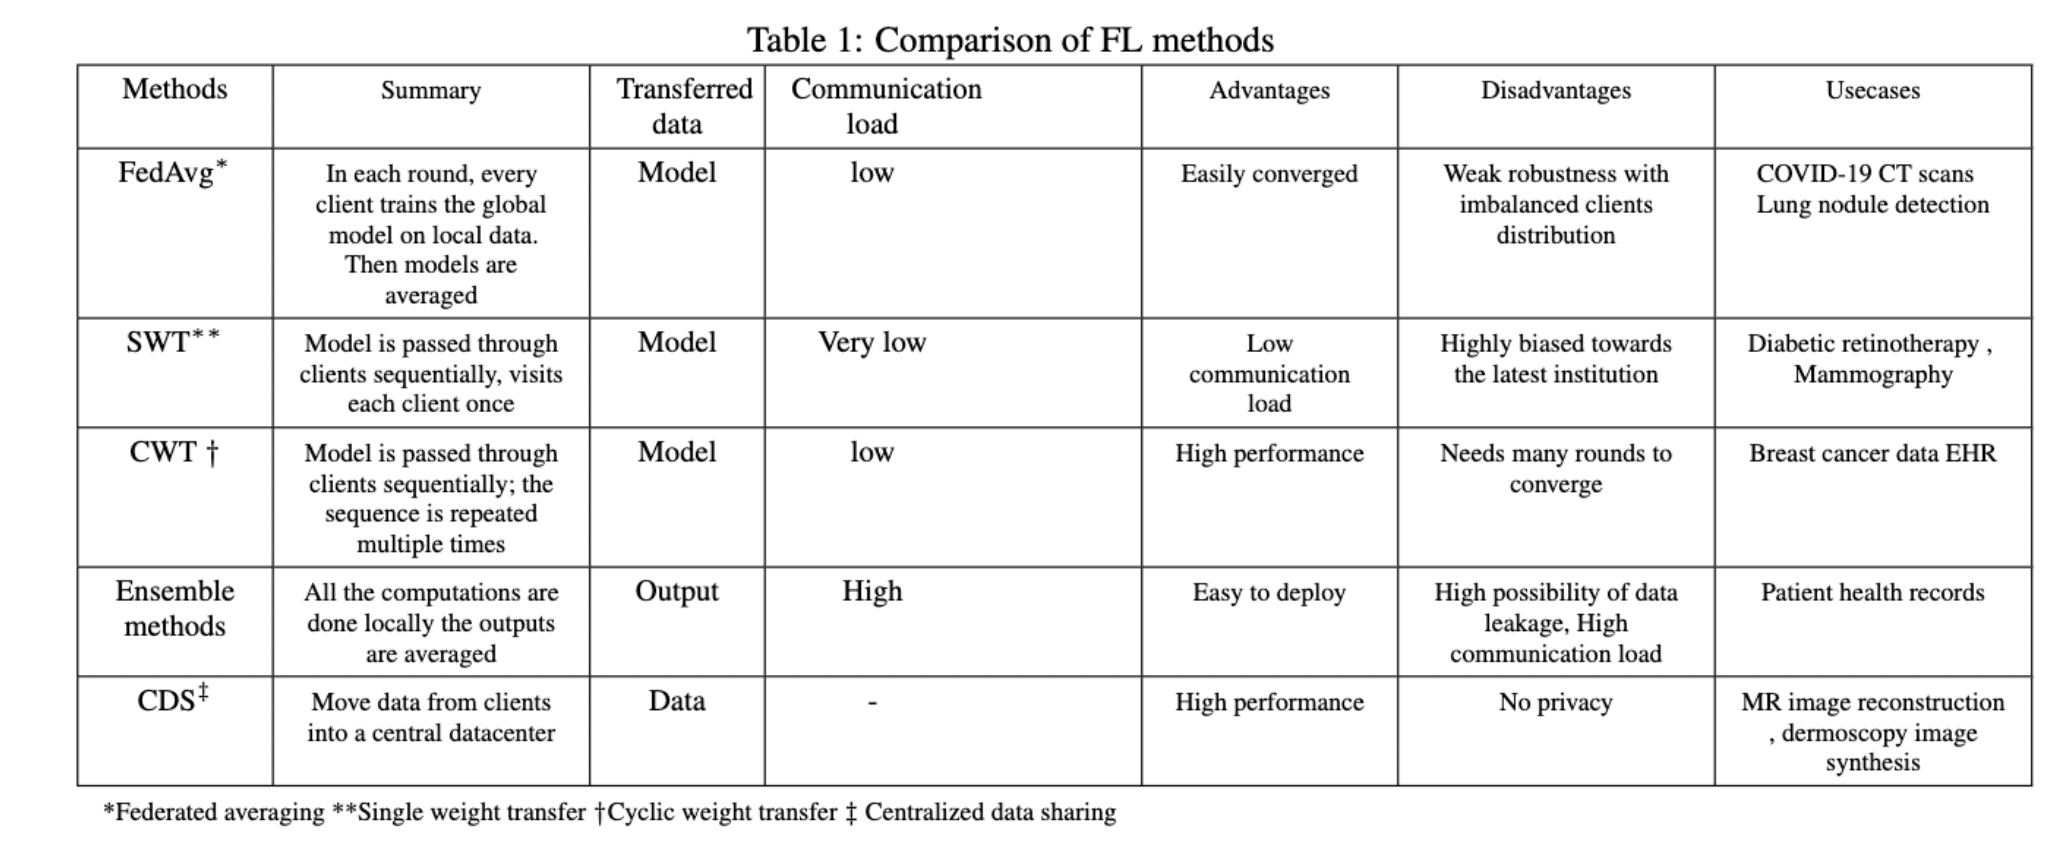
\includegraphics[scale=0.55,angle=90,origin=c]{Chapter3/Screenshot 2022-04-04 at 18.59.31.png}
%  \caption{A schema of adversarial attacks to cancer detection systems}
 \label{fig:pgd-atta-comparison}
\end{figure}

% \begin{table*}[h!]
% \centering
% \setlength{\tabcolsep}{8pt}
% \renewcommand\arraystretch{1.4}
% \caption{Result of Average Error Transfer Rate (AETR) for FGSM and PGD methods, with and without CRN initalization }
% % \begin{tabular}{cccccccccccc}
% \begin{tabular}{| *{7}{c|} }\hline
% % Dataset  & Attack type & \multicolumn{2}{c|}{ $\epsilon=0.01$} & \multicolumn{2}{c|}{ $\epsilon=0.03$}           &    \multicolumn{2}{c|}{ $\epsilon=0.05$}    & \multicolumn{2}{c|}{ $\epsilon=0.07$}                                                              \\ \hline
%  Dataset&\multicolumn{3}{c|}{ FGSM}     &              \multicolumn{3}{c|}{ PGD}                                                                           \\  

%  \cline{2-7}
% &Baseline&CRN5 &CRN10&Baeline&CRN5&CRN10\\\hline

% Meningioma&84.80\%&\textbf{86.31}\%&{84.02}\%&83.73\%  &\textbf{84.25}\%  &84.16\%\\\hline
% Glioma&82.32\% &87.06&\textbf{89.98}&74.89\%&\textbf{83.64}\% &82.32\%\\\hline

% Pathology&\textbf{90.67\%}&{84.81}\%&{85.98}\%&79.86\% &86.79\%&\textbf{86.93\%}\\\hline



% \end{tabular}
% \label{table_core} 
% \end{table*}

% \footnotesize{$^a$ The smallest spatial unit is county, $^b$ more details in appendix A}\\


% (Add the abbreviations with table legend at the bottom of the table)
On the other hand, in algorithms that transfer some type of actual data, whether distorted input data  (e.g., split learning \cite{poirot2019split}) or output data (e.g., ensemble models), the size of sent data can vary greatly depending on the data size. However, because medical imaging data is enormous, the amount of communicated information is usually more significant than with methods that transfer the model. CDS also falls into this category, as it requires actual data transfer to a central server. These two groups differ significantly in terms of communication burden as well as privacy level. Because input/output data is not sent in any format, methods which transfer models are more secure since retrieving patient data from deep learning models is difficult.

In Ensemble models, the ensembling process is done locally, and outputs of the models are sent to the global server instead of model parameters. As a result, heavy server-side computations are avoided and a federated network can be set up easily. Since ensemble models are proven to perform well in various areas of medical imaging, using ensembles can help improve the accuracy, generalizability, and stability of a federated network. However, ensemble methods impose some challenges. First, the risk of data leakage is serious in this setting. Some sort of output data like segmentation masks is very likely to reveal patients' identities. Second, contrary to model size, outputs can vary quite a lot in their size. Outputs in image format require too much communication load. 
In addition, ensemble models are design dependant. Models that do not necessarily share the same objective function can be combined into one ensemble. This leads to one complex multi-objective model having disparate optimization goals. This is not necessarily harmful, but there is a lack of research on the theoretical analysis of ensembles, and the result of an ensemble remains almost always unclear, making ensemble methods unreliable.

Besides, there is always a compromise between training time, model complexity, performance and generelizability. Altough these measures have been thoroughly investigated in single machine learning models, the literature on their relationship in a complex ensemble is still not explored much.



Another aspect of comparing FL models is that FL algorithms, in which a model is transferred, can consistently be averaged by the central server, regardless of the task they are performing. Deep neural networks performing classification, segmentation, regression, or other tasks could be averaged as long as there is a proper deep learning model for that.  All of the mentioned tasks have been demonstrated and proved to work in a federated manner. However, averaging the output from many sources is not always feasible for other federated earning algorithms. For example, if the task is multi-class classification, an ensemble approach cannot simply average the class output of distinct clients. The Ensemble approach is thus limited in the jobs it can tackle.


Several research papers have been published that compare FL implementations. Nilsson et al. \cite{nilsson2018performance} compared various FL methods in practice. They demonstrated that FedAvg is the best FL algorithm. Despite having slightly lower performance than CDS, it is practically comparable in their comparative performance analysis to a non-federated architecture.
There are numerous variants of the FedAvg algorithm and other FL approaches. However, the original FedAvg method remains one of the top methods in comparison studies. Chang et al.\cite{chang2018distributed}investigated several FL algorithms in the radiology area. According to this study, FedAvg does not impose any bias compared to other algorithms because it considers all clients equally and does not arrange them in any particular order. As shown in Figure \ref{fig:three graphs}algorithms such as SWT and CWT, clients are placed in a sequence and trained one after the other. As a result of catastrophic forgetting, the model is more representative of the most recent clients it observed and less of the earlier clients\cite{sheller2020federated}. As a result, there is a bias favoring the most recent institution in models with sequential training. Although CWT can mitigate this effect by running the model through institutions multiple times in a cyclic fashion, bias remains. Table \ref{tab:table} shows the essential characteristics of FL algorithms. There is also a sample of use cases of these algorithms in the medical domain.




Pan et al., \cite{pan2019improving},investigated the impact of the model ensemble for automatic bone age estimation based on imaging data. The results showed that combining heterogenous, uncorrelated models leads to more robust ensembles. Conversely, naively combining top models does not necessarily ensure top-notch performance.
They were able to demonstrate how data FL can aid in identifying comparable patients while protecting their privacy. 
% Another effort was made to explore the structural relationship of the brain without revealing any data. The authors used Principal component analysis (PCA) to uncover anatomical relationships between diverse datasets in a federated setup\cite{grammenos2019federated}. Federated PCA could extract features from MRI pictures from several medical institutes. Their technique was validated using several databases, including ADNI, PPMI, MIRIAD, and UK Biobank\cite{silva2019federated}.

% Balanchandar et al. \cite{balachandar2020accounting} using FL to address the issue of data variability across institutions. They used chest-Xray dataset to classify chest scans. Also, they classified retinotherapy data with their proposed method.




\section{Challenges and considerations}
\label{sec:others}

FL still has a long way to go in radiology. There are numerous challenges both in the theoretical formulation and practical implementation. FL algorithms could be divided into fully decentralized/peer-to-peer methods requiring a trusted central server. Each category comes up with its challenges. Generally speaking, methods with a central server offer more flexibility and better performance, while decentralized methods are more reliable and secure.

However, there is still some risk associated with the FL infrastructure \cite{yin2021see}. An adversary could reconstruct private data from the local model updates\cite{wang2019beyond}. Hospitals can do additional security measures to prevent adversaries from accessing the exchanged data between the server and clients.



\subsection{Data heterogeneity }


The FedAvg algorithm authors claim that their proposed method can handle heterogeneous data. However, the decentralized structure of the data makes data processing challenging to verify the completeness and quality of their findings. Further investigations revealed that this claim is not always valid\cite{li2020federated}. In almost all cases, heterogenous data deteriorates the accuracy of the FL model. The degree of divergence depends on how heterogenous the data is. Local models are trained on data with different patient profiles, resulting in a global model that could not represent all of the profiles. In some cases, heterogenous data prevents model convergence.    


Data homogeneity significantly impacts the version of the federated model to be chosen to train the model. The difference between CDS and FL might vary from similar to CDS better depending on the data. One rule of thumb would be that if data has very different distribution in different data centers, simply averaging each client's data in every round might affect the performance negatively.



Zhao et al.\cite{zhao2018federated}examined the effect of bias that distributing data can have on final performance of FL algorithms. According to their study, difference in data distribution can have negative effect on the model accuracy up to 55\%. Another difficulty is that data heterogeneity might lead to a situation where a best global model might be a poor model for some clients, or a best global model might work quite well on some clients and perform poorly on other clients. Consequently, all participants should agree on the concept of optimum model training in advance of the training. Further technical studies should be carried out to find the optimum technique for updating the central model with heterogeneous data. FedAvg is the standard method for accumulating the data from clients. Still, other distributed optimization methods that can tackle distribution differences are a subject of research.



\subsection{Bias}
Bias is a prevalent issue in distributed networks. Bias is a state that a neural network is inclined towards the distribution of a client more than other clients. It results in the model performing well on that client by compromising the performance on the other clients. The cause of bias could be the difference in the size or the distribution of clients' data. Also, the FL algorithm itself could be a source of bias.


Sheller et al.\cite{sheller2020federated}showed that CWT is a less biased algorithm than SWT. The degree of bias could vary, depending on which client was trained last.They favored FedAvg over SWT and CWT. FedAvg did the FL more fairly.  There is always a bias toward the latest clients they were trained on for algorithms like SWT and CWT. In FedAVG, however, the results of local training are aggregated every round, avoiding bias. In SWT, the global model changes after visiting each client, and succeeding clients mitigate the model's bias towards the preceding institutions. However, there is no mitigation for the latest institution the model is trained on.





The global aggregation method, i.e., server algorithm, should be designed to minimize bias . It also should be robust to local variations, as well as perturbations added by security measures. Reducing bias and designing models that capture diversity is possible by calculating the level of bias arising from each client. Then modifying the  algorithm to address the difference in the distributions. 


However, if the distribution difference is taken into account properly, bias might still emerge later in training. Some features, as well as general data distribution might vary over time.  For example, the number of patients with a particular disease in a particular hospital might change for several reasons. This can cause a domain shift: a change in a client's data distribution. There could be more work on data domain shifts and somehow explicitly address the alterations in gender, patient profile, age, and disease among different institutes or one institute. Models could also be further developed to consider economic or racial status into model training and modify a model to handle diversity in images\cite{li2020multi}. 


\subsection{Lack of standard data}
Standardizing data prevents irrelevant information from being considered meaningful in neural networks. It removes the variability between institutions.  Electronic data management is the norm in medical imaging: and medical communications (DICOM) is the globally recognized image data format and the near-global care standard for electronic file storage. However, not all the available data in the medical imaging sector is standardized. Many institutions still lack the infrastructure to handle their imaging data according to current management standards. 
One factor is the lack of a universal method to organize and manage patient records. Data management is expensive\cite{wang2003cost}. Not all hospitals have advanced data management facilities. This issue leads to the preselection of hospitals participating in research, which is a source of bias.  



Medical data are very diverse because of the diversity of modalities, dimensionalities, and features and because of variables such as variances in the acquisition, medical equipment brand, or local demographics within a specific protocol. There is still no uniform data standardization method. As a result, healthcare federated networks are likely to have clients with disparate data quality and distribution. Methods like FedAvg are generally likely to fail under these circumstances.  One way to avoid bias is to harmonize data and make each client data type similar, following a similar preprocessing. This also might require sharing metadata among institutions to find a general method of harmonization in data that suits all the institutions. But this could be tricky given the restrictions of individual institutions. Hence, one way of further development for FL systems is that the clinicians and computer scientists collaborate to standardize handling data among multiple institutions concerning the privacy restrictions and considerations.



\subsection{Privacy and Security}
Data breach is a major concern and medical data and must be safeguarded in compliance with accepted confidentiality procedures. FL has proven to be effective in protecting patients' privacy and anonymity by keeping data locally. However, there are some privacy-related challenges associated with FL. Despite many attempts to de-identify personal data from DICOM images, patient information could still be re-identified\cite{Peter2015Free} \cite{monteiro2015machine}. Recent studies have successfully rebuilt a patient's face from their MRI data. Furthermore, adversaries could steal the data or access the algorithm for non-encrypted networks. 


Furthermore, deep learning models still have some sensitive information in the weights they carry. On a decentralized network, it is feasible to reconstitute portions of patients' information only having the local model from one client\cite{carlini2019secret} \cite{zhang2020secret}
\cite{hitaj2017deep}. Adversaries can decrypt deep learning models and reveal patients' information with a very high accuracy\cite{fredrikson2015model}. Malicious parties can distort the deep learning models. False outputs produced by such models can have severe consequences if used in practice. As a result, it should be ensured that models are secure and that adversaries cannot breach models to be employed in the real-world setting\cite{tomsett2019model}.



There are specific measures to improve privacy. Particular countermeasures, such as model encryptions, Differential privacy (DP), \cite{abadi2016deep} adversarial defense against malicious clients,\cite{hitaj2017deep} and increased communication security, can be done. DP refers to the practice of keeping a dataset's global statistical distribution while minimizing individually identifiable information. DP can be done by adding perturbation to each sample.Adding noise to a dataset to reduce the chance of private data being revealed is based on the argument that one can preserve general data distribution while individual samples are changed by randomly altering a dataset. Adding systematic noise helps machine models to learn the whole distribution of training data while keeping each sample anonymous.


However, such countermeasures complicate the training algorithms and can affect training performance. Sometimes much longer training times are required, or accuracy will be dramatically decreased. This can impose an additional cost on the whole network. Hence, it is quintessential to consider whether deploying a countermeasure is necessary. The cost-efficiency of implementing them depends mainly on the level of trust among involved parties and the project scale. If clients do not trust each other, then DP is a necessity. This is because federated clients have regular communication, and critical information can be exchanged in the interactions. So each client's data should be safeguarded from other clients. This shows how important it is to clarify the level of trust among clients. This argument holds true in fully decentralized algorithms, where no central node is involved. And also in algorithms including a central server, where the client/server trust is also essential. 
Total image anonymization is still a problem. In the absence of encryption, attackers may acquire private information from local datacenters or intercept the communication pathways and rob the passing data.


\subsection{System architecture}

Medical data in federated networks requires on-premise or cloud-based data storage. Hospitals might need private or cloud-based computing power. As well as software for preprocessing and standardization of data, such as PACS. To allow the local model training hardware (GPU), connections and data centers should be set up in local centers. These bring their challenges, such as high computational power to assure harmony with other clients and high-performance bandwidth and connection between different centers, which is not always feasible in medical centers. Many hospitals still lack computing resources and strong internet connections \cite{li2010securing}. Besides, for the whole network to work correctly, redundant computational facilities and data centers should be devised to prevent data loss. If one computational client fails, the network could continue its training, which imposes an additional challenge. Robustness of the network is also critical ;federated models should be structured so that adding or removing clients and increasing or decreasing the amount of data in a center does not negatively impact patient data or model privacy.

\section{Conclusion}
 

This article introduced the main federated learning algorithms used in radiology and compared their characteristics.  
A Federated setting faces myriad challenges; designing algorithms to address them results in various algorithms with distinct optimization objectives. In general, developments focus on privacy, communication load, data heterogeneity, and model performance as their objective. This paper discusses and compares federated learning algorithms based on these objectives. We start by introducing federated learning and its paramount role in medical imaging research. Then we present the most popular federated learning algorithms and compare them.
We discuss several challenges and considerations in the next section. These challenges are current lines of research and require extra attention in implementing federated learning networks.

\printbibliography

% \bibliographystyle{unsrtnat}
% \bibliography{dissertation} 
% I hope this helps you get started!
% Moritz

\end{refsection}
% % \chapter{Challenges and considerations in Federated learning
% }
% \label{Bookchapter}

% \begin{abstract}
% \dropcap{F}ederated learning is a machine learning method that allows decentralized training of deep neural networks among multiple clients while preserving the privacy of each client's data. Federated learning is instrumental in medical imaging due to the privacy considerations of medical data. Setting up federated networks in hospitals comes with its unique challenges, primarily because medical imaging data and federated learning algorithms each have their own set of distinct characteristics. This article introduces federated learning algorithms in medical imaging and discusses technical challenges and considerations of real-world implementation of them.




% \end{abstract}

% \blfootnote{This chapter is partly based on \faFileTextO~\emph{M. Beller. Toward an
%     Empirical Theory of Feedback-Driven Development, ICSE'18 (Student Res
%     earch Competition)}~\cite{BellerSRC2018}.
% }


% \newpage

% \dropcap{T}his is a introductory page.



% keywords can be removed
% \keywords{Federated learning \and Privacy-preserving machine learning \and  Medical imaging}


\section{Introducing FL methods}

With the rapid developments in machine learning in healthcare and computer-aided diagnosis, access to medical data has become a matter of interest. Clinicians, computer scientist and medical technologists require access to more data to enable machine learning based projects. However, there is always a challenging task to balance between building more powerful machines to be used in healthcare industry, and the limitations of accessing large amount of data under the privacy considerations. Generally, sharing data requires hospitals to deal with GDPR restrictions and have an approval from the institutional review board .An institutional review board or ethical committee determines to which degree a hospital can share information with other hospitals and ensures that the GDPR restrictions are complied to. As a result , datacenters in hospitals do not usually have large and diverse datasets required to train deep neural networks. 

Federated learning (FL) \cite{mcmahan2017communication} 
is a machine learning concept proposed by McMahan et al. to tackle this problem. In this concept, a neural network is trained with datasets from multiple hospitals, and the whole training process is managed through a central server. At each round, hospitals train a neural network on their local data, and share the updated models with the central server. The server gathers all the updated models and aggregates them into an updated global model. In the next round, the updated global model is sent back to the hospitals. This way of training enables the researchers to utilize the data from multiple clients, while ensuring that the sensitive data is kept locally. 


There exist several FL algorithms.McMahan et al. \cite{mcmahan2017communication} proposed federated averaging method (FedAvG) to minimize parameter change among hospitals. The algorithm is straightforward: a subset of the clients is selected each round. Training is distributed among multiple clients. Each client will compute an updated model on their own local dataset. All model instances on the clients should start with the same random initialization to achieve convergence. Clients communicate with the central server once their local training has been finished. Finally, the central server gathers the updates of the respective clients. An immediate effect of local training can be seen at this stage. The updated global model can be tested against a test dataset, and comparing its performance with the previous round can give insight into how much improvement was achieved during the last round of training. An illustration of this step is shown in Fig. \ref{fig:train2} Blockchain-based technologies can also be used in the aggregation stage. In a blockchain network, local clients (miners) replace the central server and distribute the aggregation process among themselves. In this case, the whole process will be decentralized. Blockchain networks can be valuable since they prevent failure if the central server or clients fail.\cite{wang2021blockchain} \newpage 
\begin{figure}[h!]
 \centering
  
\includegraphics[scale=0.22]{Training step 2.jpg}
  \caption{Cloud server gathers the locally updated model from clients }
  \label{fig:train2}
\end{figure}


Another approach is averaging the outputs of the local models trained on the clients individually (ensemble single client models).A general definition for ensemble learning is different machine learning algorithms doing the same task are combined into one algorithm. Each algorithm extracts information or features from the input data, and the resulting information will be fused using various mechanisms, such as averaging, and voting. Generally, ensembles consistently outperform each of their consituting algorithms alone. In the federated setting of ensemble learning,  neither the models nor the data will be shared among clients in the training cycle. All the clients will be assigned a similar model with random initial values. Each client will train its model. Their outputs for the same task will be averaged in the deployment phase, resulting in an accumulated knowledge from multiple models.
\begin{figure}[h!]
 \centering
  
\includegraphics[scale=0.32]{Ensemble methods.jpg}
  \caption{Cloud server gathers the locally updated model from clients }
  \label{fig:train2}
\end{figure}


\begin{figure}[h!]
 \centering
  
\includegraphics[scale=0.27]{federated averaging.jpg}
  \caption{Cloud server gathers the locally updated model from clients }
  \label{fig:train2}
\end{figure}


\begin{figure}[h!]
 \centering

\includegraphics[scale=0.3]{SWT.jpg}  \caption{Cloud server gathers the locally updated model from clients }
  \label{fig:train2}
\end{figure}


\begin{figure}[h!]
 \centering

\includegraphics[scale=0.3]{CWT algorithm.jpg}
\caption{Cloud server gathers the locally updated model from clients }
  \label{fig:train2}
\end{figure}


% \begin{figure*}
%      \centering
%      \begin{subcaption}[b]{0.23\textwidth}
%          \centering
%          
\includegraphics[scale=0.32]{Ensemble methods.jpg}
%          \caption{}
%          \label{fig:y equals x}
%      \end{subcaption}
%      \hfill
%      \begin{subfigure}[b]{0.23\textwidth}
%          \centering
%          
\includegraphics[scale=0.27]{federated averaging.jpg}
%          \caption{}
%          \label{fig:three sin x}
%      \end{subfigure}
%      \\ [10pt]
%      \centering
%     %  \hfill
%      \begin{subfigure}[b]{0.21\textwidth}
%          \centering
%          \raisebox{\dimexpr\ht\imagebox-\height}{ \includegraphics[scale=0.3]{SWT algorithm.jpg}}
        
%          \caption{}
%          \label{fig:five over x}
%      \end{subfigure}
%     %  \hspace{0.2\textwidth}
%      \hfill
%      \begin{subfigure}[b]{0.21\textwidth}
%          \centering
%         %  \hfill
%          
\includegraphics[scale=0.3]{CWT algorithm.jpg}
%          \caption{}
%          \label{fig:five over x}
%      \end{subfigure}
%         \centering
%         \captionsetup{justification=centering}
%         \caption{Schema of different decentralized learning methods, (a) Ensemble methods, clients train local models on their own dataset,model outputs of different clients are averaged. (b) FedAvg, an initial model is sent to the clients, each train the model on their own data and the resulting local models are averaged in a central server. (c) SWT, an initial model is sequentially passed through clients and visit each clients once. Final model is the model trained on the latest client. (d) CWT, similar to SWT, however, model is passed through institutions multiple times.}
%         \label{fig:three graphs}
% \end{figure*}




A third algorithm is single weight transfer (SWT). In this algorithm, a deep learning model is trained at a single client up to a particular time and then transferred to the next client. There are numerous options to decide when to finish a local training and pass its model to the next client.  Standard criteria are the number of epochs per client and validation loss or accuracy depending on the problem. For example,  Chang et al. \cite{chang2018distributed} chose to reach the plateau of validation loss as a sign of moving to the next client.  Cyclic weight transfer (CWT) is another algorithm in which a model is trained at each client for a predetermined number of epochs, then transferred to the next client. In this algorithm, the model visits each client than once. 

The functionality of models and tasks in an FL scenario differs depending on the FL algorithm. Algorithms that transfer models are more versatile and adaptable than other algorithms. Deep learning models' performance in a federated environment can also vary from model to model. Models' adaptability can determine the overall performance of an FL network. For example, research has shown that some deep neural network components (such as batch normalization layers) cause performance issues and are harder to adjust in a federated setup. On the other hand, components like convolutional layers could be easily averaged, averaging their results in a proper global model.  As a result, deep learning models that have more suitable components are a better choice for FL. Reseach is going on to develop specific models that perform better in a federated environment\cite{li2021fedbn}.



\subsection{Comparison of the federated learning algorithms}
We may categorize the algorithms based on what is exchanged between the server and the client to compare federated algorithms. Techniques such as FedAVG, SWT, and CWT, transfer the model between the server and the clients. Approaches like split learning \cite{poirot2019split}  transfer middle layer outputs of a neural network. The middle layer outputs can be regarded as a distorted form of the input data. In other words, as the neural network processes the input data, it undergoes numerous modifications that distort the input. Methods such as ensemble methods share their models' final output and broadcast it to a central server. 

The amount of data transferred is relatively tiny in methods in which the model is moved to the central server and is independent of the amount of training data at each site. It is solely determined by the size of the deep learning model. The majority of popular deep learning algorithms are tens of megabytes in size. However, an FL algorithm that transfers a model does not necessarily have a low overall communication overhead. The overall amount of exchanged data also depends on the number of communication rounds between clients and servers. The hyperparameters can determine the number of communication rounds, and communication overhead could be high if there is too much exchange between clients.



% \begin{table*}[h!]
% \centering
% \setlength{\tabcolsep}{8pt}
% \renewcommand\arraystretch{1.4}
% \caption{Result of Average Error Transfer Rate (AETR) for FGSM and PGD methods, with and without CRN initalization }
% % \begin{tabular}{cccccccccccc}
% \begin{tabular}{| *{7}{c|} }\hline

% \setlength\tabcolsep{0pt}
% \begin{table}[h!]
% 	\caption{Comparison of FL methods}
% 	\centering
% 	\setlength{\tabcolsep}{0pt}
%     \renewcommand\arraystretch{1}
%   	\begin{tabular}{|p{0.07} | p{0.05}|p{0.06} |p{0.05}|p{0.10} |p{0.05}|p{0.13} |} \newline
% 		 Methods & Summary & Transferred data & Communication load & Advantages &	Disadvantages &	Usecases \newline
% 		FedAvg$^{*}$ & In each round, every client trains the global model on local data. Then models are averaged &Model &	low	&Easily converged&Weak robustness  with imbalanced clients distribution&COVID-19 CT scans \cite{dou2021federated}
% 		Lung nodule detection  \cite{baheti2020federated} 
%  \newline \hline
%  SWT$^{**}$ &
% 		Model is passed through clients sequentially,visits each client once	&Model&	Very low&	Low communication load&	Highly biased towards the latest institution &	Diabetic retinotherapy  \cite{chang2018distributed}, Mammography  \cite{chang2018distributed}

%       \newline \hline
% 	CWT $\dagger$ &	Model is passed through clients sequentially; the sequence is repeated multiple times&Model&low&High performance&	Needs many rounds to converge&Breast cancer data\cite{beaulieu2018privacy} EHR \cite{beaulieu2018privacy}

%   \newline \hline
% 		Ensemble methods&All the computations are done locally the outputs are averaged&Output&High&Easy to deploy&	High possibility of data leakage, High communication load&Patient health records \cite{li2016distributed} 

%  \newline \hline
% 		CDS$^{\ddagger}$&Move data from clients into a central datacenter&Data&-&High performance&No privacy&MR image reconstruction \cite{Quan2018compressed} , dermoscopy image synthesis \cite{DBLP:journals/corr/abs-1804-03700}
%   \\ \hline
%   \multicolumn{4}{l}{*Federated averaging **Single weight transfer    ${\dagger}$Cyclic weight transfer   $\ddagger$ Centralized data sharing } \\
% 	\end{tabular}
% 	\label{tab:table}
% \end{table}
%     % \begin{tabular}{ll}
%     % \end{tabular}

\begin{table*}[h!]
\centering
\setlength{\tabcolsep}{8pt}
\renewcommand\arraystretch{1.4}






\label{table_core} 
\end{table*}

\begin{figure}[t!]
 \centering
 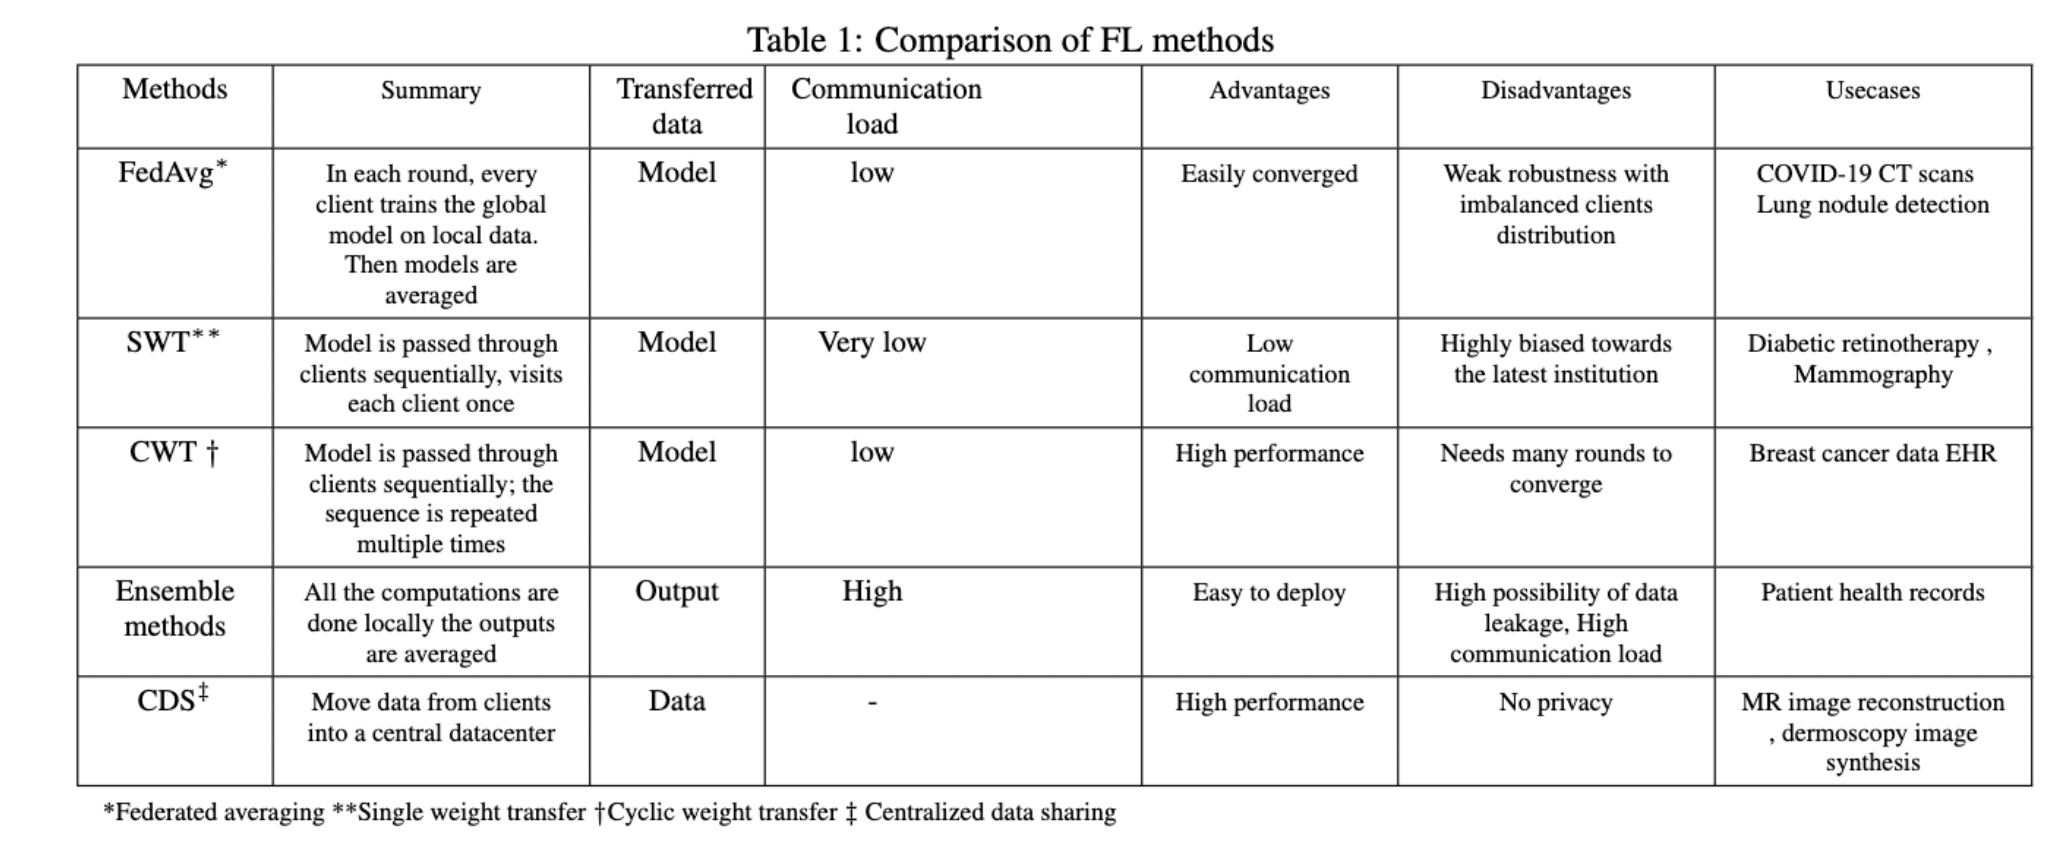
\includegraphics[scale=0.55,angle=90,origin=c]{Chapter3/Screenshot 2022-04-04 at 18.59.31.png}
%  \caption{A schema of adversarial attacks to cancer detection systems}
 \label{fig:pgd-atta-comparison}
\end{figure}

% \begin{table*}[h!]
% \centering
% \setlength{\tabcolsep}{8pt}
% \renewcommand\arraystretch{1.4}
% \caption{Result of Average Error Transfer Rate (AETR) for FGSM and PGD methods, with and without CRN initalization }
% % \begin{tabular}{cccccccccccc}
% \begin{tabular}{| *{7}{c|} }\hline
% % Dataset  & Attack type & \multicolumn{2}{c|}{ $\epsilon=0.01$} & \multicolumn{2}{c|}{ $\epsilon=0.03$}           &    \multicolumn{2}{c|}{ $\epsilon=0.05$}    & \multicolumn{2}{c|}{ $\epsilon=0.07$}                                                              \\ \hline
%  Dataset&\multicolumn{3}{c|}{ FGSM}     &              \multicolumn{3}{c|}{ PGD}                                                                           \\  

%  \cline{2-7}
% &Baseline&CRN5 &CRN10&Baeline&CRN5&CRN10\\\hline

% Meningioma&84.80\%&\textbf{86.31}\%&{84.02}\%&83.73\%  &\textbf{84.25}\%  &84.16\%\\\hline
% Glioma&82.32\% &87.06&\textbf{89.98}&74.89\%&\textbf{83.64}\% &82.32\%\\\hline

% Pathology&\textbf{90.67\%}&{84.81}\%&{85.98}\%&79.86\% &86.79\%&\textbf{86.93\%}\\\hline



% \end{tabular}
% \label{table_core} 
% \end{table*}

% \footnotesize{$^a$ The smallest spatial unit is county, $^b$ more details in appendix A}\\


% (Add the abbreviations with table legend at the bottom of the table)
On the other hand, in algorithms that transfer some type of actual data, whether distorted input data  (e.g., split learning \cite{poirot2019split}) or output data (e.g., ensemble models), the size of sent data can vary greatly depending on the data size. However, because medical imaging data is enormous, the amount of communicated information is usually more significant than with methods that transfer the model. CDS also falls into this category, as it requires actual data transfer to a central server. These two groups differ significantly in terms of communication burden as well as privacy level. Because input/output data is not sent in any format, methods which transfer models are more secure since retrieving patient data from deep learning models is difficult.

In Ensemble models, the ensembling process is done locally, and outputs of the models are sent to the global server instead of model parameters. As a result, heavy server-side computations are avoided and a federated network can be set up easily. Since ensemble models are proven to perform well in various areas of medical imaging, using ensembles can help improve the accuracy, generalizability, and stability of a federated network. However, ensemble methods impose some challenges. First, the risk of data leakage is serious in this setting. Some sort of output data like segmentation masks is very likely to reveal patients' identities. Second, contrary to model size, outputs can vary quite a lot in their size. Outputs in image format require too much communication load. 
In addition, ensemble models are design dependant. Models that do not necessarily share the same objective function can be combined into one ensemble. This leads to one complex multi-objective model having disparate optimization goals. This is not necessarily harmful, but there is a lack of research on the theoretical analysis of ensembles, and the result of an ensemble remains almost always unclear, making ensemble methods unreliable.

Besides, there is always a compromise between training time, model complexity, performance and generelizability. Altough these measures have been thoroughly investigated in single machine learning models, the literature on their relationship in a complex ensemble is still not explored much.



Another aspect of comparing FL models is that FL algorithms, in which a model is transferred, can consistently be averaged by the central server, regardless of the task they are performing. Deep neural networks performing classification, segmentation, regression, or other tasks could be averaged as long as there is a proper deep learning model for that.  All of the mentioned tasks have been demonstrated and proved to work in a federated manner. However, averaging the output from many sources is not always feasible for other federated earning algorithms. For example, if the task is multi-class classification, an ensemble approach cannot simply average the class output of distinct clients. The Ensemble approach is thus limited in the jobs it can tackle.


Several research papers have been published that compare FL implementations. Nilsson et al. \cite{nilsson2018performance} compared various FL methods in practice. They demonstrated that FedAvg is the best FL algorithm. Despite having slightly lower performance than CDS, it is practically comparable in their comparative performance analysis to a non-federated architecture.
There are numerous variants of the FedAvg algorithm and other FL approaches. However, the original FedAvg method remains one of the top methods in comparison studies. Chang et al.\cite{chang2018distributed}investigated several FL algorithms in the radiology area. According to this study, FedAvg does not impose any bias compared to other algorithms because it considers all clients equally and does not arrange them in any particular order. As shown in Figure \ref{fig:three graphs}algorithms such as SWT and CWT, clients are placed in a sequence and trained one after the other. As a result of catastrophic forgetting, the model is more representative of the most recent clients it observed and less of the earlier clients\cite{sheller2020federated}. As a result, there is a bias favoring the most recent institution in models with sequential training. Although CWT can mitigate this effect by running the model through institutions multiple times in a cyclic fashion, bias remains. Table \ref{tab:table} shows the essential characteristics of FL algorithms. There is also a sample of use cases of these algorithms in the medical domain.




Pan et al., \cite{pan2019improving},investigated the impact of the model ensemble for automatic bone age estimation based on imaging data. The results showed that combining heterogenous, uncorrelated models leads to more robust ensembles. Conversely, naively combining top models does not necessarily ensure top-notch performance.
They were able to demonstrate how data FL can aid in identifying comparable patients while protecting their privacy. 
% Another effort was made to explore the structural relationship of the brain without revealing any data. The authors used Principal component analysis (PCA) to uncover anatomical relationships between diverse datasets in a federated setup\cite{grammenos2019federated}. Federated PCA could extract features from MRI pictures from several medical institutes. Their technique was validated using several databases, including ADNI, PPMI, MIRIAD, and UK Biobank\cite{silva2019federated}.

% Balanchandar et al. \cite{balachandar2020accounting} using FL to address the issue of data variability across institutions. They used chest-Xray dataset to classify chest scans. Also, they classified retinotherapy data with their proposed method.




\section{Challenges and considerations}
\label{sec:others}

FL still has a long way to go in radiology. There are numerous challenges both in the theoretical formulation and practical implementation. FL algorithms could be divided into fully decentralized/peer-to-peer methods requiring a trusted central server. Each category comes up with its challenges. Generally speaking, methods with a central server offer more flexibility and better performance, while decentralized methods are more reliable and secure.

However, there is still some risk associated with the FL infrastructure \cite{yin2021see}. An adversary could reconstruct private data from the local model updates\cite{wang2019beyond}. Hospitals can do additional security measures to prevent adversaries from accessing the exchanged data between the server and clients.



\subsection{Data heterogeneity }


The FedAvg algorithm authors claim that their proposed method can handle heterogeneous data. However, the decentralized structure of the data makes data processing challenging to verify the completeness and quality of their findings. Further investigations revealed that this claim is not always valid\cite{li2020federated}. In almost all cases, heterogenous data deteriorates the accuracy of the FL model. The degree of divergence depends on how heterogenous the data is. Local models are trained on data with different patient profiles, resulting in a global model that could not represent all of the profiles. In some cases, heterogenous data prevents model convergence.    


Data homogeneity significantly impacts the version of the federated model to be chosen to train the model. The difference between CDS and FL might vary from similar to CDS better depending on the data. One rule of thumb would be that if data has very different distribution in different data centers, simply averaging each client's data in every round might affect the performance negatively.



Zhao et al.\cite{zhao2018federated}examined the effect of bias that distributing data can have on final performance of FL algorithms. According to their study, difference in data distribution can have negative effect on the model accuracy up to 55\%. Another difficulty is that data heterogeneity might lead to a situation where a best global model might be a poor model for some clients, or a best global model might work quite well on some clients and perform poorly on other clients. Consequently, all participants should agree on the concept of optimum model training in advance of the training. Further technical studies should be carried out to find the optimum technique for updating the central model with heterogeneous data. FedAvg is the standard method for accumulating the data from clients. Still, other distributed optimization methods that can tackle distribution differences are a subject of research.



\subsection{Bias}
Bias is a prevalent issue in distributed networks. Bias is a state that a neural network is inclined towards the distribution of a client more than other clients. It results in the model performing well on that client by compromising the performance on the other clients. The cause of bias could be the difference in the size or the distribution of clients' data. Also, the FL algorithm itself could be a source of bias.


Sheller et al.\cite{sheller2020federated}showed that CWT is a less biased algorithm than SWT. The degree of bias could vary, depending on which client was trained last.They favored FedAvg over SWT and CWT. FedAvg did the FL more fairly.  There is always a bias toward the latest clients they were trained on for algorithms like SWT and CWT. In FedAVG, however, the results of local training are aggregated every round, avoiding bias. In SWT, the global model changes after visiting each client, and succeeding clients mitigate the model's bias towards the preceding institutions. However, there is no mitigation for the latest institution the model is trained on.





The global aggregation method, i.e., server algorithm, should be designed to minimize bias . It also should be robust to local variations, as well as perturbations added by security measures. Reducing bias and designing models that capture diversity is possible by calculating the level of bias arising from each client. Then modifying the  algorithm to address the difference in the distributions. 


However, if the distribution difference is taken into account properly, bias might still emerge later in training. Some features, as well as general data distribution might vary over time.  For example, the number of patients with a particular disease in a particular hospital might change for several reasons. This can cause a domain shift: a change in a client's data distribution. There could be more work on data domain shifts and somehow explicitly address the alterations in gender, patient profile, age, and disease among different institutes or one institute. Models could also be further developed to consider economic or racial status into model training and modify a model to handle diversity in images\cite{li2020multi}. 


\subsection{Lack of standard data}
Standardizing data prevents irrelevant information from being considered meaningful in neural networks. It removes the variability between institutions.  Electronic data management is the norm in medical imaging: and medical communications (DICOM) is the globally recognized image data format and the near-global care standard for electronic file storage. However, not all the available data in the medical imaging sector is standardized. Many institutions still lack the infrastructure to handle their imaging data according to current management standards. 
One factor is the lack of a universal method to organize and manage patient records. Data management is expensive\cite{wang2003cost}. Not all hospitals have advanced data management facilities. This issue leads to the preselection of hospitals participating in research, which is a source of bias.  



Medical data are very diverse because of the diversity of modalities, dimensionalities, and features and because of variables such as variances in the acquisition, medical equipment brand, or local demographics within a specific protocol. There is still no uniform data standardization method. As a result, healthcare federated networks are likely to have clients with disparate data quality and distribution. Methods like FedAvg are generally likely to fail under these circumstances.  One way to avoid bias is to harmonize data and make each client data type similar, following a similar preprocessing. This also might require sharing metadata among institutions to find a general method of harmonization in data that suits all the institutions. But this could be tricky given the restrictions of individual institutions. Hence, one way of further development for FL systems is that the clinicians and computer scientists collaborate to standardize handling data among multiple institutions concerning the privacy restrictions and considerations.



\subsection{Privacy and Security}
Data breach is a major concern and medical data and must be safeguarded in compliance with accepted confidentiality procedures. FL has proven to be effective in protecting patients' privacy and anonymity by keeping data locally. However, there are some privacy-related challenges associated with FL. Despite many attempts to de-identify personal data from DICOM images, patient information could still be re-identified\cite{Peter2015Free} \cite{monteiro2015machine}. Recent studies have successfully rebuilt a patient's face from their MRI data. Furthermore, adversaries could steal the data or access the algorithm for non-encrypted networks. 


Furthermore, deep learning models still have some sensitive information in the weights they carry. On a decentralized network, it is feasible to reconstitute portions of patients' information only having the local model from one client\cite{carlini2019secret} \cite{zhang2020secret}
\cite{hitaj2017deep}. Adversaries can decrypt deep learning models and reveal patients' information with a very high accuracy\cite{fredrikson2015model}. Malicious parties can distort the deep learning models. False outputs produced by such models can have severe consequences if used in practice. As a result, it should be ensured that models are secure and that adversaries cannot breach models to be employed in the real-world setting\cite{tomsett2019model}.



There are specific measures to improve privacy. Particular countermeasures, such as model encryptions, Differential privacy (DP), \cite{abadi2016deep} adversarial defense against malicious clients,\cite{hitaj2017deep} and increased communication security, can be done. DP refers to the practice of keeping a dataset's global statistical distribution while minimizing individually identifiable information. DP can be done by adding perturbation to each sample.Adding noise to a dataset to reduce the chance of private data being revealed is based on the argument that one can preserve general data distribution while individual samples are changed by randomly altering a dataset. Adding systematic noise helps machine models to learn the whole distribution of training data while keeping each sample anonymous.


However, such countermeasures complicate the training algorithms and can affect training performance. Sometimes much longer training times are required, or accuracy will be dramatically decreased. This can impose an additional cost on the whole network. Hence, it is quintessential to consider whether deploying a countermeasure is necessary. The cost-efficiency of implementing them depends mainly on the level of trust among involved parties and the project scale. If clients do not trust each other, then DP is a necessity. This is because federated clients have regular communication, and critical information can be exchanged in the interactions. So each client's data should be safeguarded from other clients. This shows how important it is to clarify the level of trust among clients. This argument holds true in fully decentralized algorithms, where no central node is involved. And also in algorithms including a central server, where the client/server trust is also essential. 
Total image anonymization is still a problem. In the absence of encryption, attackers may acquire private information from local datacenters or intercept the communication pathways and rob the passing data.


\subsection{System architecture}

Medical data in federated networks requires on-premise or cloud-based data storage. Hospitals might need private or cloud-based computing power. As well as software for preprocessing and standardization of data, such as PACS. To allow the local model training hardware (GPU), connections and data centers should be set up in local centers. These bring their challenges, such as high computational power to assure harmony with other clients and high-performance bandwidth and connection between different centers, which is not always feasible in medical centers. Many hospitals still lack computing resources and strong internet connections \cite{li2010securing}. Besides, for the whole network to work correctly, redundant computational facilities and data centers should be devised to prevent data loss. If one computational client fails, the network could continue its training, which imposes an additional challenge. Robustness of the network is also critical ;federated models should be structured so that adding or removing clients and increasing or decreasing the amount of data in a center does not negatively impact patient data or model privacy.

\section{Conclusion}
 

This article introduced the main federated learning algorithms used in radiology and compared their characteristics.  
A Federated setting faces myriad challenges; designing algorithms to address them results in various algorithms with distinct optimization objectives. In general, developments focus on privacy, communication load, data heterogeneity, and model performance as their objective. This paper discusses and compares federated learning algorithms based on these objectives. We start by introducing federated learning and its paramount role in medical imaging research. Then we present the most popular federated learning algorithms and compare them.
We discuss several challenges and considerations in the next section. These challenges are current lines of research and require extra attention in implementing federated learning networks.

\printbibliography

% \bibliographystyle{unsrtnat}
% \bibliography{dissertation} 
% I hope this helps you get started!
% Moritz

\begin{refsection}
\chapter{A Comparative Study of Federated Learning Methods for COVID-19 Detection}

\label{Bookchapter}

\begin{abstract}
\dropcap{D}eep learning has proven to be highly effective in diagnosing COVID-19; however, its efficacy is contingent upon the availability of extensive data for model training. The data sharing among hospitals, which is crucial for training robust models, is often restricted by privacy regulations. Federated learning (FL) emerges as a solution by enabling model training across multiple hospitals while preserving data privacy. However, the deployment of FL can be resource-intensive, necessitating efficient utilization of computational and network resources. In this study, we evaluate the performance and resource efficiency of five FL algorithms in the context of COVID-19 detection using Convolutional Neural Networks (CNNs) in a decentralized setting. The evaluation involves varying the number of participating entities, the number of federated rounds, and the selection algorithms. Our findings indicate that the Cyclic Weight Transfer algorithm exhibits superior performance, particularly when the number of participating hospitals is limited. These insights hold practical implications for the deployment of FL algorithms in COVID-19 detection and broader medical image analysis.

\end{abstract}
\newpage

\section{Background and Related works}

 % $\Delta W_n^t$
 
Federated learning has demonstrated efficacy in an array of imaging modalities, including Magnetic Resonance Imaging (MRI) \cite{sheller2020federated}\cite{silva2019federated}, X-ray \cite{balachandar2020accounting}, retinal imaging \cite{balachandar2020accounting}, as well as in applications such as brain tumor segmentation \cite{bakas2017advancing}\cite{lee2018privacy}, diagnosis \cite{pan2019improving}, and treatment selection \cite{lee2018privacy}. In particular, Federated Learning (FL) has proven to be a valuable tool for supporting physicians in their decision-making process regarding the treatment of COVID-19 patients. A landmark study that involved 20 institutions across five continents found that FL played a significant role in shaping patient treatment plans\cite{flores2021federated}. The study employed chest radiography images in conjunction with clinical information to determine the appropriate level of care and oxygen requirements for patients afflicted with COVID-19. It was observed that FL improved the performance of the predictive model, especially for institutions with smaller datasets, compared to using only local data for model training. Additionally, it was found that healthcare facilities with smaller datasets often had underrepresented categories due to a low number of patients in certain classes. The implementation of FL led to a notable improvement in predictions for these underrepresented patient categories.

\begin{figure*}[t!]
\centering
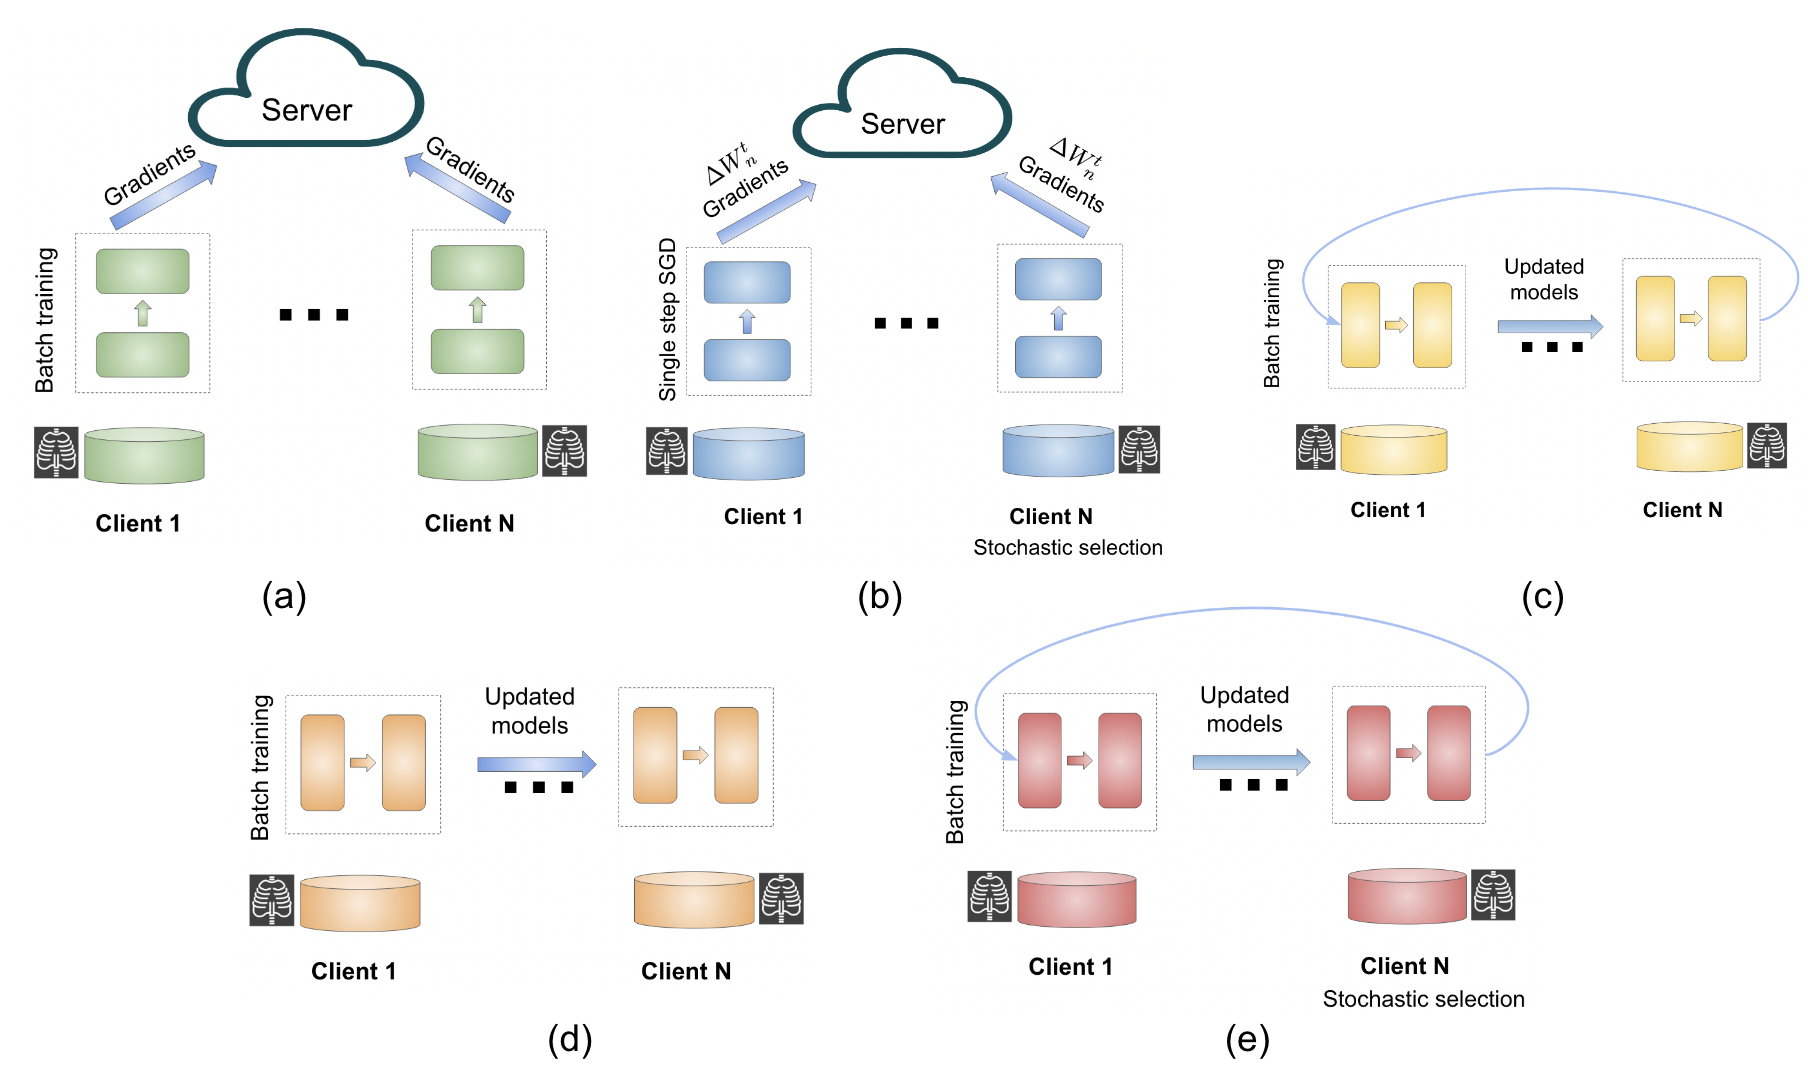
\includegraphics[width=1\textwidth]{FLmodels.png}
\caption{Illustration of FL models and algorithms: (a) Federated averaging, where clients train on a local batch of data. (b) FedSGD, in which a subset of clients is selected, and each performs a single step of SGD before sending model updates to the server. (c) Cyclic Weight Transfer (CWT), where clients train locally and pass the model to the next client, repeating the cycle. (d) Single Weight Transfer (SWT), where the model passes through each client only once. (e) Stochastic Weight Transfer (STWT), in which the model is sequentially passed through clients, with participating clients in each round being sampled randomly.}
\label{fig:flalgorithms}
\end{figure*}


Recent research has focused on the classification of scan images to distinguish between COVID-19 patients and healthy individuals, as well as identifying lesion areas. The primary application of AI in managing COVID-19 patients has been the interpretation of radiology images, especially chest CT scans.  The detection of lung alterations through these scans plays an important role in optimizing patient management and guiding treatment decisions\cite{yan2020interpretable}\cite{hu2020challenges}\cite{burian2020intensive}.  Several studies have also explored 3D Convolutional neural networks \cite{wang2020weakly} and COVID-19 detection with a limited number of training samples.

While the majority of these studies report favorable accuracy, they often presume a centralized environment wherein a single data center has access to all data. However, a few studies have successfully applied distributed learning for COVID-19 detection, employing global aggregation models such as model averaging in federated learning settings\cite{ho2022fedsgdcovid}\cite{zhang2021dynamic}, or within a blockchain framework \cite{kumar2021blockchain}. These studies have pointed to certain limitations of existing algorithms, such as high communication overhead \cite{remedios2020federated}, as well as convergence issues or catastrophic forgetting when the number of participating hospitals increases \cite{sheller2020federated} \cite{chang2018distributed}.


To our knowledge, no study has been performed that compared multiple FL algorithms under standard conditions to evaluate their applicability. Therefore, comparing multiple FL algorithms under standard conditions could be informative in evaluating their applicability in practice.

To evaluate the existing methods from multiple perspectives, we have implemented the most popular models and compared them in terms of performance, communication overhead, and computation burden.


\section{Algorithms}
% \label{sec:algorithms}
\textbf{Centralized Data Sharing} In Centralized Data Sharing (CDS), data is stored in a central location and is accessible to all clients. This stands in contrast to federated and decentralized data sharing methods, where data is stored across multiple locations and accessed by either a single user or a limited number of users. CDS serves as a baseline for comparing other algorithms.
\textbf{Federated Averaging} Federated Averaging involves an iterative learning procedure comprising local and global steps. In this process, each data owner trains a model received from a global server on its local dataset through local iterations \cite{mcmahan2017communication}. Subsequently, the global server aggregates the updated local models to update the global model. This global model is then distributed to clients for the subsequent round. The optimization problem for Federated Averaging can be expressed as:
\begin{equation}
w^{t+1} = \sum\limits_{i=1}^{N}{p_{i} w_{i}^{t}} , w_{i}^{t}=\arg\min\limits_{w_{i}}{\left(\mathcal{L}(\mathcal{D}_{i};w^{t})\right)}
\end{equation}
where $N$ is the number of data owners, $\mathcal{L}(\mathcal{D}_{i};w^{t})$ is a loss function indicating global model parameters  $w^{t}$ of local datasets, and $p_{i}$ is the probability of selecting client $i$. 
Local optimization can be formulated as $w_{i}^{t+1} \leftarrow w^{t}-\eta\cdot \nabla \mathcal{L}(w^{t};\mathcal{D}_{i})$, where 
 $\eta$ is the learning rate. The global model can be updated based on the local models $w_{i}$ and is shared for aggregation: 
\begin{equation}
w^{t+1} = \sum\limits_{i=1}^{N}{p_{i} w_{i}^{t+1}}
\end{equation}

\textbf{Federated Stochastic Gradient Descent} Federated Stochastic Gradient Descent, or FedSGD\cite{chai2020fedeval}, is a variant of Federated Averaging (FedAvg) that employs a large-batch synchronous approach for multi-client learning. In FedSGD, a subset of clients is chosen from the total pool, with this subset being defined by $C$. This selection is made at each global round. Subsequently, the global server dispatches the latest global model to the chosen clients. Each of these clients then undertakes local training on its dataset for a predetermined number of epochs. The global model is updated in light of the local models obtained from each client and is made available for aggregation, a process that is analogous to that in FedAvg. Nevertheless, FedSGD distinguishes itself by computing the gradient over the chosen batch of clients, hence $C < 1$. When $C = 1$, the training becomes non-stochastic, or full batch, as it involves all the clients. This makes it possible to train with large batches since the gradient is computed over the selected subset of clients.

The optimization problem for FedSGD can be expressed as follows:
\begin{equation}
w^{t+1} = w^{t} - \eta \cdot \sum\limits_{i=1}^{C}p_i \cdot \nabla \mathcal{L} (w^t;\mathcal{D}_i)
\end{equation}
where $\eta$ is the learning rate, $p_i$ is the probability of selecting client $i$ and $\mathcal{L}$ is the loss function.
The key difference between FedAvg and FedSGD lies in the use of large-batch synchronous approach in FedSGD. This approach has been shown to outperform the naive asynchronous SGD training due to the increased accuracy and efficiency, as compared to the local training approach used in FedAvg \cite{chai2020fedeval}\cite{charles2021large}. Additionally, FedSGD has been shown to be more robust to non-IID data distributions, compared to FedAvg \cite{chai2020fedeval}. 
\quickthings{This part is unclear to me.}
% \absolutelynecessary{}
\maybelater{paraphrised}

\textbf{Cyclic weight transfer} Federated learning techniques have been widely used in medical image processing tasks using a method known as cyclic weight transfer (CWT)\cite{balachandar2020accounting}. This method involves training models on individual clients for a number of iterations and then cyclically sharing the updated weights with the following client. However, the existing CWT algorithm faces a notable challenge, as it lacks the ability to effectively manage inter-client variability in training data or labels.  To ensure the practical application of CWT, it is crucial to develop a version that can handle the common variations observed in a majority of real-world medical imaging datasets\cite{darzidehkalanifederatedII}.

\textbf{Single weight transfer} Single weight transfer (SWT) is anothe FL method widely used in the medical imaging domain. In Single weight transfer, models are trained in each client with its local data, and then the updated model is transferred to the next client. The difference between this method and CWT is that here the model passes each client only once\cite{darzidehkalanifederatedI}. 

\textbf{Stochastic weight transfer}
In stochastic weight transfer (STWT), we select a subsample of clients and train them in a cyclic manner. Similar to FedSGD, a ratio defines the number of selected clients to the total number of clients in each federated round. 

Figure \ref{fig:flalgorithms} provides a visual representation of the introduced algorithms.



% سوال / مسیله چیه
% Importance: Why your research matters in the context of an industry or the world
% اهمیت موضوع
% 	کجاها کاربرد داره
% مشکلات موضوعات قبلی و اینکه مسایل دگ کار نمیکنن
% برای اینکه این مسایل کار کنن نیازی به چه چیزی بود. ک اونا کم داشتن
% چرا این روش تو داره کار میکنه
% چه سوالی رو جواب میده
% توضیح اینکه چجوری کار میکنه
% تعریف و تمجید از کار کردنش

% \maybelater{chanta akse tamiz ba coreldraw bekesh}

% Their
% We are comparing various implementations of FL and comparing their performance level. The performance is done by metrics.
% 2. Although FL has been introduced to tackle the problem of privacy, its distributed nature requires too much commuincation between clients. Knowsing can determine its deployability and scailibitlty. Hence the question is how to these model compare it terms of communication between clients.
% 3. Computation time. Each FL model is investigated based on the required time for computation.
% 4. Effect of rounds: Number of Federated rounds 


% \quickthings{Maybe you can add a benchmarking section similar to "A Performance Evaluation of FL Algorithms"}
% \maybelater{Some ideas are herer https://arxiv.org/pdf/1709.05929.pdf
% }





 
\section{Experiment}
\textbf{Dataset} Our experiments used two publicly available data sources, the Tongji hospital dataset\cite{yang2020covid} and Brazil's SARS-CoV-2 dataset\cite{soares2020sars} Tongji dataset consists of 349 chest CT-scans of COVID-19 positive and 397 scans of healthy subjects, all low-resolution CT modalities. Brazil's SARS-CoV-2 dataset consists of 2482 samples, 1252 scans of COVID-19-infected patients, and 1230 healthy subjects collected from multiple hospitals in Sao Paulo, Brazil. The datasets are approved by the corresponding ethical committees of each hospital, Public Hospital of Sao Paulo (HSPM), and Tongji Hospital in Wuhan, China. Train and test sets were obtained randomly from the aggregated datasets. Table \ref{table_datadist}, shows data distribution.


\begin{table}[h!]
\centering
\setlength{\tabcolsep}{6pt}
\renewcommand\arraystretch{1.22}
\caption{ \small Data distribution}
\begin{tabular}{| *{5}{c|} }
\hline
Class  & Dataset & Samples & Train & Test
\\   \hline  
\multirow{2}{3em}{COVID}     &Brazil&1252&\multirow{2}{2em}{1451}  &\multirow{2}{2em}{150}  \\
&Tongji&349&&  \\
\hline
\multirow{2}{6em}{Non-COVID}     &Brazil&1230&\multirow{2}{2em}{1477}  &\multirow{2}{2em}{150}  \\
&Tongji&397&&  \\
\hline
\end{tabular}
\label{table_datadist} 
\end{table}


\textbf{Preprocessing}
Images were selected as 2D slices in greyscale. Preprocessing included randomly cropping between 0.5 to full size, random horizontal flipping, and intensity normalization. CT-slices were all resized to 224$\times$224 pixels with interpolation. Figure \ref{fig:samplesCTs} shows samples of processed images.
% \quickthings{This looks like you have a bias in your dataset. You should select the normals and abnormals at comparable level in the thorax. All covid are now lower in the body then the non-covid ones.}
% \maybelater{I have changed the picture, hope it's okay now}
\begin{figure}[h!]
 \centering
 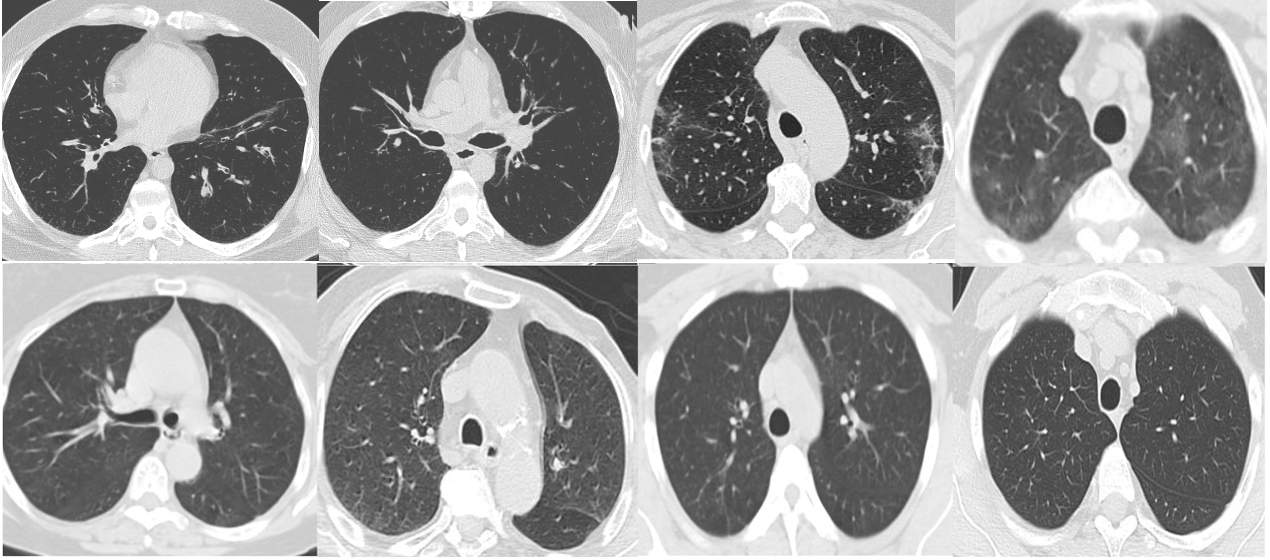
\includegraphics[width=0.45\textwidth]{covidexamples3.png}
 \caption{Sample CT slices of COVID-19 images (top row) and Non-COVID images (bottom row)}
 \label{fig:samplesCTs}
\end{figure}


% normalize = transforms.Normalize(mean=[0,0,0], std=[1,1,1])
% train_transformer = transforms.Compose([
%     transforms.Resize(256),
%     transforms.RandomResizedCrop(224, scale=(0.5, 1.0)),
%     transforms.RandomHorizontalFlip(),
%     transforms.ToTensor(),
%     normalize
% ])

\textbf{Training}
ResNet-18 is used as the backbone deep learning model. ResNet-18 comprises one initial block cascaded to four middle blocks. The initial block is made of convolutional,  batch normalization, ReLU, and pooling layers. Middle blocks have the same layers, connected with straight and skip connections. The model is pre-trained on ImageNet dataset \cite{he2016deep} with a CrossEntropy loss function and learning rate of $0.05$. 
Each federated round consisted of 20 internal epochs for each client and batches of 16 samples in each iteration. For models which use minibatch training, like STWT and FedSGD, a subset of clients is randomly selected. Similar to training, test data was split into mini-batches, and the results were averaged across batches. We performed training with various participating clients and federated rounds to evaluate their effect on final performance. Models were also trained in a centralized, non-federated setting to build a comparison baseline. Figure \ref{fig:distributionsite} shows the data distribution among clients.

\begin{figure}[h!]
 \centering
 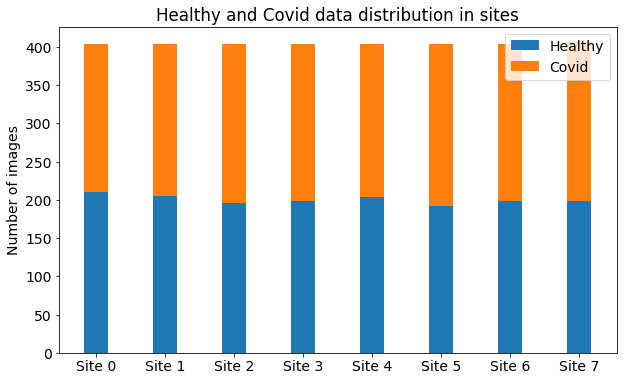
\includegraphics[width=0.7\textwidth]{output.png}
 \caption{Data distribution of each client in the simulated federated setting}
 \label{fig:distributionsite}
\end{figure}
% \abs{Healthy COVID data distirbution per site}

\textbf{Evaluation} 
Standard classification metrics, accuracy, recall, precision, and F1 score, were used as our evaluation criteria. We also evaluated the level of communication, the amount of transferred data in each algorithm, and the computational complexity of the models. 
\label{sec:experiment}


\section{Results}


% In order to evaluate and compare federated learnign models 
% Specificity  and  sensitivity  are  the  abilities  of  a  model  that how correctly the model identifies a subject with disease and without a disease. 
% In our case, it is critical to detect a COVID-19 patient as missing a COVID-19 patient can have disastrous consequences.   

% A medical diagnosis based system needs to have high sensitiv- ity and recall. 
Here, the result for the setting with 10 participating clients and a maximum of 10 rounds is presented. The results are average performance among clients for all the federated rounds. Table \ref{best_performance} shows the results.
% \quickthings{Why comparison of FedAVG and CWT?}\maybelater{I removed the sentence}
% The average score in each state could be a way to reach them—the average scores in F1, FedSGD, CWT, and SWT. 
% The FedSGD models have been used are
% The results for CDS are also included as a benchmark ground truth.

% \quickthings{Put CDS at the top, keep same order as in the materials and methods. Consistency!}
% \maybelater{Fixed!}

\begin{table}[h!]
\centering
\setlength{\tabcolsep}{5.5pt}
\renewcommand\arraystretch{1.12}
\caption{ \small Comparison of FL algorithms on classification of COVID-19 data for 10 clients, averaged performance in all the 10 rounds.}
\begin{tabular}{| *{5}{c|} }
\hline
Method & Accuracy & Recall & Precision & F1 score
\\
  \hline
  

CDS
 &87.75\%&89.57\% &87.93\% & 87.19\%  
\\   \hline  
FedAVG
 & 66.72\% &70.02\% &43.80\% & 51.7\%\\ 
 \hline  
FedSGD
 &65.17\% &68.24\%&43.86\%& 47.75\%  
 
 \\
 \hline  
CWT
 &87.75\%&89.00\%& 88.67\%&87.52\%\\
 
   \hline
 

SWT
 & 64.60\% &74.33\% & 65.55\% &59.66\% \\
    
\hline 
STWT
 & 84.21\% &84.09\%&83.33\% & 81.71\%  \\



\hline
\end{tabular}
\label{best_performance} 
\end{table}


\textbf{Assesing the impact of training rounds} To evaluate the effect of number of rounds, models with 3, 5, 10 and 15 rounds were tested. The test results are shown for both centralized and FL  algorithms. Table \ref{number_of_rounds} shows the results of our experiment. The increasing number of rounds correlates with higher accuracy of the global model.
% \quickthings{Same with table III, put at the top.}

% \maybelater{done}

% \begin{table}[h!]
% \centering
% \setlength{\tabcolsep}{5.5pt}
% \renewcommand\arraystretch{1.12}
% \caption{ \small Effect number of rounds on models' accuracy}
% \begin{tabular}{| *{5}{c|} }
% \hline
% Method & 3 rounds & 5 rounds & 10 rounds & 15 rounds 
% \\   \hline  
% FedAVG
%  & 66.28\% &77.24\% & 86.63\% & 94.03\%\\

%  \hline
%  FedSGD
%  &  53.77\% & 70.55\% &90.04\% & 92.75\%\\
% \hline  
% % SWT
% %  &  85.34\% & 97.24\% &93.63\% & 98.74\%\\
% % \hline  
% CWT
%  &  96.02\% & \textbf{98.44\%} &\textbf{99.29\%} & 99.86\%\\

% % \hline  
% % CDS
% %  to be completed!


% \hline  
% STWT
%  &  \textbf{96.59\%} & 97.72\% &99.57\% & \textbf{100.00\%}\\

 
%  \hline
% CDS
%  &92.03\% &88.34\% & 98.01\% & 100.00\% \\
%  \hline
% \end{tabular}
% \label{number_of_rounds} 
% \end{table}


\begin{table}[h!]
\centering
\setlength{\tabcolsep}{3.5pt}
\renewcommand\arraystretch{1.12}
\caption{ \small Effect number of rounds on accuracy of FL algorithms for 10 clients, 20 internal epochs.}
\begin{tabular}{| *{5}{c|} }

% \begin{tabular}{| {c|}{c|}{c|}{c|}{c|}{c|}{c|}{c|}{c|} |}
\hline
% Method & \multicolumn{2}{c}{3 rounds} & \multicolumn{2}{c}{5 rounds} &\multicolumn{2}{c}{10 rounds} &\multicolumn{2}{c}{15 rounds} 

Method & 3 rounds & 5 rounds & 10 rounds & 15 rounds
%  & M &SD & M &SD& M &SD& M &SD 
\\
 \hline
CDS
 &85.06\% &81.56\% & 91.06\% & 91.04\% 
\\
\hline
FedAVG
 & 56.05\%  &63.78\%&69.64\%&70.73\% \\

 \hline
 FedSGD
 &  50.88\% & 55.9\% &75.59\% & 76.94\%\\
% \hline  
% SWT
%  &  85.34\% & 97.24\% &93.63\% & 98.74\%\\
\hline  
CWT
 &  80.77\% & \textbf{89.78\%} &\textbf{91.27\%}& \textbf{93.56\%}\\

% \hline  
% CDS
%  to be comp,';leted!


\hline  
STWT
 &  \textbf{90.73\%} & 83.97\% &89.44\% & 93.01\%\\

 
  \hline

\end{tabular}
\label{number_of_rounds} 
\end{table}
\quickthings{Shouldn't this column have the same results as table II for accuracy?}

\peter{Table III and Table II do not represent the same thing. Table II is average performance in all 10 rounds, is to give an overall impression of accuracy, and table III is the final result in the end of the 5th, 10th , 15th rounds.  Added  to the table caption.
}
% \maybelater{The results are for max, maybe you want to add average results later?}
% \maybelater{Having the same thing (acc) for other metrics such as F1, prevciison recall etc}

\textbf{Assessing the influence of client participation}
To evaluate the number of clients on the FL network, we examined scenarios with 3,5, and 8 participating clients. We trained each of the clients in 20 internal epochs. The number of Federated rounds for all the algorithms (except SWT) was 10.
The average test results are shown in the Figure \ref{fig:data distribution}. \quickthings{Why not a column for 10 clients here?}
\maybelater{ 10 clients are shown in table three , third column. Added 10 clients here as well}

% \begin{table}[h!]
% \centering
% \setlength{\tabcolsep}{7pt}
% \renewcommand\arraystretch{1.22}
% \caption{ \small Effect number of clients on accuracy of FL algorithms, 10 rounds, 20 internal epochs.}
% \begin{tabular}{| *{9}{c|} }
% \hline
% Method & 3 clients & 5 clients & 8 clients 
% \\   \hline  
% FedAVG
%  & 79.52\% &70.73\% & 63.98\% \\

% \hline  
% FedSGD
%  & 78.02\% &75.59\% &69.76\%  \\
% \hline  
% CWT
%  &  89.90\% & \textbf{91.27\%} &\textbf{88.98\%} \\
%  \hline
% STWT
%  &  \textbf{90.93\%} & 89.44\% &84.57\% \\
%  \hline  
% SWT
%  & 55.80\% &69.19\% & 68.81\%\\




% \hline  
% CDS
%  to be completed!

% \hline  

% \end{tabular}
% \label{effect_num_clients} 
% \end{table}


\begin{figure}[h!]
 \centering
 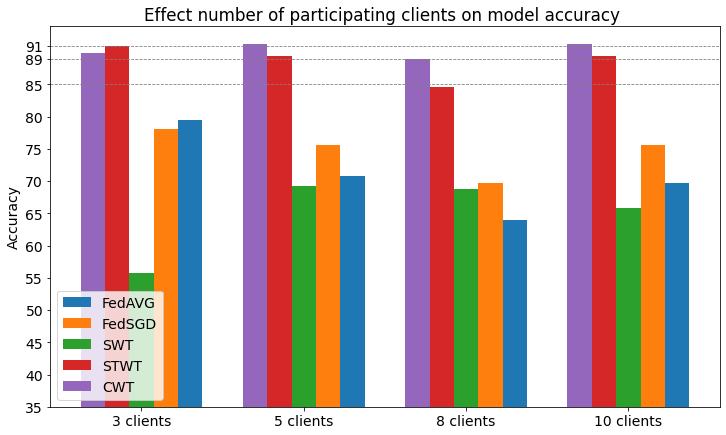
\includegraphics[width=0.7\textwidth]{download.png}
 \caption{Accuracy of FL algorithms with differrent number of clients. }
 \label{fig:data distribution}
\end{figure}


% \maybelater{Maybe taking MAX is better instead of latest epoch?}

 
\begin{figure}[h!]
 \centering
 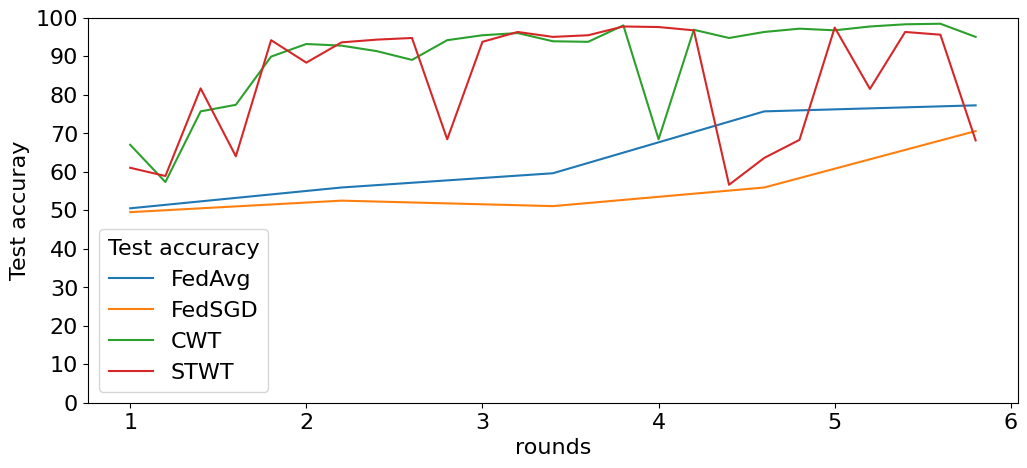
\includegraphics[width=0.7\textwidth]{cyclic.png}
 \caption{Test accuracy as a function of passing rounds}
 \label{seq-vs-noseq}
\end{figure}
% \maybelater{Best accuracy vs Average accuracy for showing that SWTW works bad in average but well in best accuracy}
% \abs{Adding a graph showing arrows for gradient updates}
% \maybelater{Maybe adding 10 clients?}
% \maybelater{8 ta client, 4 FL rounds
% 20 each client for CWT plot . and also 8 ta client, 4 FL round 20 each client for FedSGD and FedAVG}
% \subsection{Other graphs}

\begin{table}[h!]
\label{computation time}
\centering
\setlength{\tabcolsep}{7pt}
\renewcommand\arraystretch{1.22}
\caption{ \small Computation time (seconds) for FL algorithms for standardized setting}
\begin{tabular}{| *{9}{c|} }
\hline
Method & 3 clients & 5 clients & 8 clients  & 10 clients
\\   \hline  
FedAVG
 & 8934 sec&8975 sec  & 9002 sec & 9030 sec\\

\hline  
FedSGD
 & 8810 sec &8853 sec& 9013 sec & 9052 sec \\
\hline  
CWT
 &  5119 sec& 5450 sec&5383 sec & 5556 sec\\
 \hline
STWT &
2805 sec&  5243 sec& 6101 sec & 6129 sec\\
 \hline  
SWT
 & \textbf{543 sec} &\textbf{547 sec} & \textbf{589 sec } & \textbf{618 sec}\\



% \hline  
% CDS
%  to be completed!

\hline  

\end{tabular}
\label{computation_time} 
\end{table}


Communication can also be a bottleneck in this setting. In methods like federated averaging, the lower bounds for total communicated data are proportional to $\sim$
${2NT}$
where the total rounds are represented by T and the count of involved clients is denoted by N. In CWT, this lower bound is  $\sim$ ${NT}$. In our setting, we use a ResNet 101 model. We calculated the overall transferred data for the different number of rounds. As expected, the experiments show that when clients are selected randomly, the communication time tends to be shorter compared to scenarios involving participation from all clients. Moreover, our analysis of computational costs indicates that models that do not rely on sequential processing generally demand higher computational resources compared to their sequential counterparts. The detailed results for computational and communication evaluations can be found in Table \ref{computation_time} and Table \ref{transferredData}, respectively.
\quickthings{Again, why only this comparison is relevant enough to put into the text?}
\maybelater{Here fedavg, and fedsgd are the same family, (non sequential), and CWT are the other family (sequential)., Changed the phrasing from CWT/FedAVG to seq/non-seq, hope it's okay this time.}

\begin{table}[h!]
\centering
\label{Transferred data}
\setlength{\tabcolsep}{5.5pt}
\renewcommand\arraystretch{1.12}
\caption{ \small Comparison of total transferred data in a normalized setting (GB)}
\begin{tabular}{| *{5}{c|} }
\hline
Method & 3 rounds & 5 rounds & 10 rounds & 15 rounds 
\\   \hline  
FedAVG
 & 1.371 &2.286 & 4.571 & 6.857\\

 \hline
 FedSGD
 &  0.823 & 1.371 &2.743 & 4.114\\
\hline  
% SWT
%  &  85.34\% & 97.24\% &93.63\% & 98.74\%\\
% \hline  
CWT
 &  0.686 & 1.143 &2.286 & 3.428\\

% \hline  
% CDS
%  to be completed!


\hline  
STWT &
  0.411 & 0.686 &1.371 & 2.057\\

 

 \hline
\end{tabular}
\label{transferredData} 
\end{table}





% \maybelater{Momkene computational complexity ro beshe ba order nevesht? peida kon settingesh ro}
% \maybelater{Graphs showing results}
% \maybelater{Comparison of FL models}
% \maybelater{Loss/round}
% \abs{definition of precision and recall}


\label{sec:results}



% % \newpage

 
\section{Discussion}
\label{sec:discussion}

% Local training had near random accuracy, but in all the experiments, the performance results were improved. 
% Considering low number of samples for individual clients, a training process limited to few clients results in near random classification accuracy. 
% Local models can have low performance due to limited datasets.
% Also,, ImageNet pre-training had a speed-up effect on our model performance.

% \textbf{Fundamental groups of FL}

% \textbf{how many groups}
% \textbf{how can we group them, name different ways}
% \textbf{effect number of data}


% Paragraph 1: This paragraph provides a “big picture” perspective for readers to remind them of the importance of your study.

% \textbf{overall results}
% 
Our results show that FL has comparable performance to centralized data sharing, with the advantage of keeping data private. With large volumes of data and after high number of rounds, centralized data sharing and cyclic weight transfer have the highest accuracy. 


Sequential models are susceptible to catastrophic forgetting, where a global model performs well on the latest client it has seen while having poor performance in other clients.\quickthings{cryptic sentence}\maybelater{I have paraphrised the sentence}
Conversely, in algorithms like FedAvg and FedSGD, the models are averaged asynchronously after all the clients have finished their training. So the trajectory is smoother and overall improving with more communication rounds. As shown in Figure \ref{seq-vs-noseq}, local test results can have a high variance when passing through clients sequentially, indicating the catastrophic forgetting effect.

Models like FedAvg, and FedSGD, in which all the clients have identical copies of one global model, are slower and more challenging to converge compared to sequential models like CWT and STWT. Also, FedAvG and FedSGD require more training resources due to active server participation, resulting in more computation and network consumption. Stochastic client selection is an efficient way of training. Stochastic models save significant time and resources while having similar performance to full client participation. Overall, CWT and STWT have best results in terms of model accuracy and computation times. These findings could be practical in further federated deployments in medical institutions.
% but when there are communication and computation limitations, other methods might be more practical.




% As can be seen in the results, CWT and STWT have better local results than other methods.

% So each local model is different than other models, and even in fewer rounds they retrain the model on their local data and achieve high accuracies. 

%  Unsurprisingly, CDS has higher accuracy than non-sequential methods.
 
% so in limited number of rounds, latter algorithms are preferred.



%  FedAVG needs to perform both local training and global aggregation, which requires is to have more computation, than sequential models which eliminate global aggregation and broadcasting step.   
%  Models with global server, suh as FedAVG and FedSGD, required more data transfer, because of the two way communication of each client with server.
Sequential models like CWT and STWT perform better than non-sequential models on fewer training rounds. For example,  after three rounds of training, STWT and CWT both reach 96\% accuracy, while FedAvG reaches 66\%, and FedSGD performs equally to a random classifier. As the training proceeds, FedAVG and FedSGD gradually improve with more global rounds.The concept of sequential models is similar to fine-tuning \cite{chen2020online} in centralized deep learning, so in cases where a hospital temporarily joins an FL network, or there is an urgency in training, sequential models are a better option.

More training rounds do not always lead to a better global model. Although average performance on all clients improves, more global rounds lead to worse performance for some clients. The global model can overfit some clients, leading to lower performance on others\cite{mohri2019agnostic}. Some studies suggested early stopping and fine-tuning to local dataset after global training is finished \cite{yu2020salvaging}. 
In all the algorithms, more clients resulted in slower convergence. This effect is stronger in the FedAvg algorithm. In FedAVG, the Global model must compromise between potentially disparate local minima\cite{li2019convergence}. Methods such as adaptive or stochastic selection of clients and momentum-based models help faster convergence \cite{liu2020accelerating}.
Our results suggest that stochastic client participation is close to full client participation. The average results of four trials with varying rounds, shown in Table \ref{number_of_rounds} indicate that stochastic client participation in FedSGD results in 5.23\% performance loss and 40\% less bandwidth consumption compared to FedAvg. In STWT, it results in only 1.25\% less accuracy but saves 40\% of communication and 11.3\% of computation.
% Also, SWT improves local clients' performance up to 80\% accuracy with 8 clients, and it requires extremely low bandwidth requirements.
These results are in accordance with prior studies, showing that, in theory, stochastic and full client participation have similar global minima\cite{cho2020client}. Stochastic client selection can be advantageous when there are limited resources, or in larger networks with occasionally unavailable clients.


% Models like FedSgd and STWT, select the participating clients in a stochastic manner. 
% The reason is because each client has less data, and there will be more number distant local client minima leading to unstable global model.


% Such can be a reflection of real world setting, where not all the clients are active in each round. So a fraction are selected.


% Some models have high max test accuracy while average is low indicating bias and catastrophic forgetting. Infrastructure limitations should be considered, when a central server has limited computing power it would be unable to perform FedAVG, instead no-server algorithms require to pass the model to the next client.

We did not assume any shift in clients' data. A more comprehensive analysis should consider the effect of the domain and distribution shifts on the performance of the algorithms. Also, inter-client data variability and the effect of heterogenous clients could be a future line of research.
% For deployments in longer timeframes, there might be changes in clients data distirbution , and previous results might be inapplicable Effect of domain shifts, and inter-client data variability could be a future line of research. 






\section{Conclusion}
\label{sec:conclusion}
 
FL enables extensive collaborations of hospitals to address medical imaging problems while keeping data private. Real-world implementation requires consideration of efficiency and hardware requirements in addition to model performance, especially in the healthcare field, which generally has limited infrastructure. We implemented five FL algorithms for COVID-19 detection and analyzed their efficiency and accuracy.
Our results suggest that FL algorithms have comparable performance to centralized data sharing, with the advantage of keeping data private. They also show that the sequential methods are a better option in most of the scenarios. This study can be helpful in the deployment of FL systems in COVID-19 detection and medical image analysis in general.

% demonstrate better performance for detecting COVID-19 patients and might be practical in deploying FL algorithms for covid-19 detection and medical image analysis in general.





\printbibliography


% \section{Introduction}
% TBD
% \section{Methods}
% TBD
% \section{Results}
% TBD
% \section{Discussion and conclusion}
% TBD
% \section{References}

\end{refsection}

\part{Security of federated networks in medical imaging}

\begin{refsection}

\chapter{Adversarial attacks on federated learning networks
for medical image analysis}
\label{Bookchapter}

\begin{abstract}
\dropcap{F}ederated learning (FL) can significantly mitigate privacy concerns for Medical image analysis (MIA) systems. However, its decentralized and collaborative nature can bring new attack surfaces which might impose severe threats for participating clients.  
This paper investigates adversarial attacks where the adversary tries to fool other clients with manipulated data. 
% We presume a differentially private setting where the adversary has no access to other clients' models and data.
We investigate the credibility of known threat factors in a federated environment and discuss their importance. We demonstrate that domain-specific settings can lead to higher attacker success on MRI tumor and pathology imaging datasets.
In addition, we propose a scenario in which the adversary leverages the federated environment to devise a more powerful attack. We show that using gradient information from previous global model updates enables single-step attacks (e.g., FGSM) to outperform computationally expensive iterative methods so that the adversary reaches the same success rate $20 to 30$ times faster.



\end{abstract}

\blfootnote{This chapter is partly based on \faFileTextO~\emph{M. Beller. Toward an
    Empirical Theory of Feedback-Driven Development, ICSE'18 (Student Res
    earch Competition)}~\cite{BellerSRC2018}.
}


\newpage

% \dropcap{T}his is a introductory page.



% keywords can be removed
% \keywords{Federated learning \and Privacy-preserving machine learning \and  Medical imaging}


% \section{Introduction}

\section{Introduction}
\IEEEPARstart{I}n the past few years, federated learning (FL) has emerged as one of the mainstream machine learning (ML) paradigms and gained much attention in the field of medical image analysis (MIA). Federated learning enables hospitals and other healthcare providers to train machine learning models jointly with other hospitals without sharing sensitive data. It is applied to a wide scope of MIA tasks, successfully addressing data governance concerns. Notable works include brain tumor classification and segmentation, breast density classification, and covid-19 detection. \cite{sheller2020federated,dayan2021federated,rieke2020future}.



Although FL has mitigated many risks and concerns about multi-institutional collaborations, it is still vulnerable to other privacy issues. Several emerging attacks are proven to threaten FL networks. Adversarial clients might be able to change the model's prediction or gain information about other clients by actively changing its own model parameters or synthesizing fake input data.





This paper analyzes a group of attack scenarios called 'adversarial attacks.' A malicious client aims to cheat the model by adding subtle noise to its examples. The noise is so minimal that the change in the image is imperceptible for a human observer. However, it can cause the model to misclassify it. 
Adversarial attacks are the main source of vulnerability to the deployed FL models \cite{bouacida2021vulnerabilities,lyu2020threats,costa2021covert,lyu2020privacy}\. and are designed to fool the models that  are already trained 
% So their threat for the deployment phase 
passed their test phase and delivered for clinical use. 
% \\Although there is some research in the past in FL and MI, we believe that adversarial attacks could also be explored since they could be a threat to clinical decision-making.
% \\The attacks are analyzed in a federated setting to investigate their inter-client transferability.
\\We leverage the FL environment to propose a stronger attack and show that it enables adversarial clients to manipulate other benign clients to a high degree.  
We also show that proposed defense methods such as differential privacy still have limited effect against this attack.
In the following sections, we introduce adversarial attacks, sources of vulnerability, and our method.

\begin{figure}[t!]
 \centering
 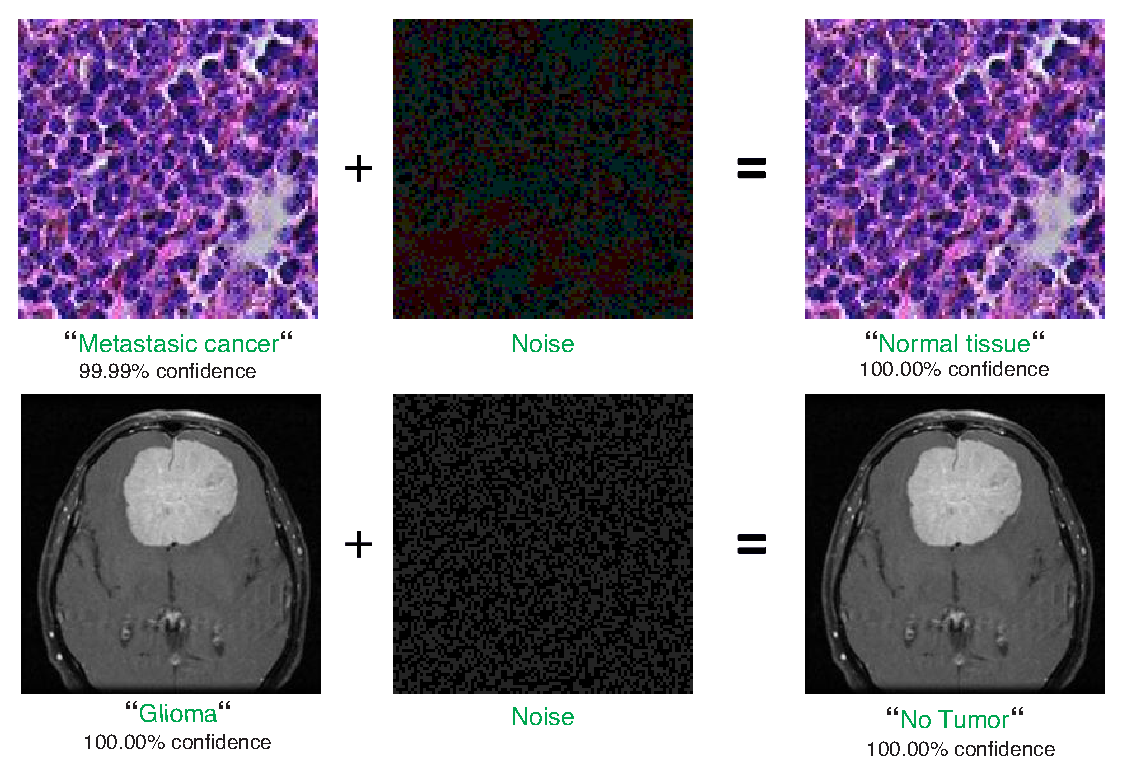
\includegraphics[width=0.52\textwidth]{Whatisads.eps}
 \caption{A schema of adversarial attacks to cancer detection systems}
 \label{fig:pgd-atta-comparison}
\end{figure}
 
 

%  Even if in indirect use and as a backbone for imaging software.
 \subsection{ Adversarial attacks }
Adversarial attacks are attributed to the linear characteristics of high-dimensional data. \cite{goodfellow2014explaining}. The crafted noise examples produced using one model might be able to manipulate other models. In FL setting, these attacks are also known as evasion attacks.\cite{biggio2013evasion,costa2021covert,ayub2020model,bouacida2021vulnerabilities}, are defined as if a malicious client tries to manipulate other clients with fake data.\\
At the same time, research on defense methods is also ongoing. Some studies tried to incorporate differential privacy (DP) as a protection measure in FL setting. Differential privacy was initially proposed to protect against privacy attacks, but it has also been applied against adversarial attacks.\cite{bouacida2021vulnerabilities,asgari2018vulnerability,wu2020evaluation}. Despite the ongoing research, there is no universal defense method against them.

We have introduced adversarial attacks in the scope of FL and MIA systems. We argue that distinct features of FL environments and MI make their combination highly vulnerable to adversarial attacks. \cite{chen2017targeted,chen2019deepinspect,ji2018model}.  The following paragraphs argue how each FL and MI expose new attack surfaces.
\\\textbf{Federated learning and adversarial attacks:} FL characteristics are known to elevate the impact of attacks known in the centralized setting. \cite{goldblum2020dataset,liu2022threats} The unique vulnerabilities of FL can be :
% We think the adversarial attacks on federated learning medical systems are notable important for three reasons, and this topic might not be explored properly. 
\begin{enumerate}[(i)]

\item{\textit{More data:} }
Each model received in every round has updated information about other clients. Adversaries can exploit this information to prepare stronger attacks.\cite{sun2019can,fang2020local,wang2020attack,song2020analyzing}
\item \textit{Open training:} In FL, the training process involves a lot of participants. Among them, one adversary could act maliciously.
\item{\textit{Standardized data pipelines:}} FAIR data stations and data standardization steps are inherent in many of FL networks in hospitals\cite{wilkinson2016fair}, near Global 
Electronic data management and medical communications (DICOM) integrated into the federated pipelines.
\cite{van2022ai}. Clients with more similar data are prone to attacks. \cite{miotto2016deep}
\item \textit{Scale of deployments:} FL networks have been deployed on a large scale in healthcare. Models act as a backbone of multiple inference software. FL networks in the deployment stage are especially weak against adversarial attacks. \cite{costa2021covert,bouacida2021vulnerabilities}.

\end{enumerate}
\textbf{Medical images and adversarial attacks}: Also, medical images have distinct features which makes the networks trained on them more vulnerable.
\begin{enumerate}[(i)]
    \item {\textit{Feature representation:}} Due to the inherent feature space of medical images, MIA systems are more vulnerable to this sort of attack than natural images. As shown in  previously published work, medical images have a narrower high-dimensional feature representation of images than natural images, causing trained networks to be over-parameterized. \cite{ma2021understanding} Over-parameterized networks are inherently easier to fool. \cite{Ye_2019_ICCV} As a result, medical imaging classifiers are easier to fool than natural image classifiers.  \cite{ma2021understanding} Several works have confirmed this by arbitrarily manipulating Funduscupy, Chest X-Ray and Dermoscopy data resulting in ... \cite{finlayson2019adversarial}. 
    \item \textit{Unique texture:}Medical images have limited texture diversity, and small texture perturbation in medical images can confuse classifiers to a high degree. \cite{ma2021understanding} This feature can be of advantage to the adversary's attacks, because they can perturb the texture in irrelevant areas and fool the classifier without manipulating the more important parts, e.g., the tumor area.\cite{ma2021understanding}. Which has, for example, been shown to effectively confuse tumor detection classifiers  \cite{gupta2022vulnerability}
    
\end{enumerate}



\subsection{Transferability factors}
Despite defense not always being an option, DL systems might be able to gain insight into their points of vulnerability. Some parameters and deployment settings might increase the chances of a successful attack.\\
Gaining such perception can be directly imported in security analysis so that the technicians know where the highest threat can be from, and they do not require a brute-force simulation of all the scenarios and parameter values, which is practically hard and in most cases impossible. 
\\The research is ongoing on attack transferability.\cite{gao2022boosting,elaalami2022bod,dai2021fast,duan2022novel,du2020hybrid,zheng2020efficient,shafahi2019adversarial,qiu2022framework}. In the MIA domain, transferability analysis has been done in a centralized ML setting, and the results are found to be domain specific. Factors such as data disparity, perturbation degree, and pre-training are shown to be crucial in attack transferability. However, their extent and optimal values might vary to a large extent. This difference can be attributed to the characteristics of the target imaging domain, texture of images, and whether the attack is white-box or black-box.\cite{ma2021understanding} \cite{bortsova2021adversarial}. \\ In an FL setup with a higher level of complexity, their findings might have limited pertinence. \cite{costa2021covert} One research question could be how FL can bring up new factors, and whether its optimal attack settings are concordant with the existing literature obtained from centralized data experiments. 
In this project we investigated potential factors in this setup, and discuss their effect on transferability.




\\\subsection{Our attack}

The adversarial client participating in an FL setup has access to previous model updates. We investigate a scenario where the adversary can enhance its attack using the gradient information from those model updates. However, obtaining gradient information might be a challenge, and also transferring them to the subsequent models causes drastic parameter change.\cite{zheng2020efficient}
We introduce an intermediary noise tensor we call \textit{Cross-round noise (CRN)} which utilizes previously received global model updates to generate noise and passes them to the next FL round. To initialize the next round and avoid parameter change, we regularize $L_{2}$ each noise channel by its mean value. 
\\This way can achieve better performance and improve transferability, with a much lower computation burden than the standard attack methods. %This can boost the computationally expensive attack models and bring higher capability.

% We assumed that the attacker doesn't necessarily have knowledge about model weights or inner settings of the target model, or the softwares that are build upon the model.\\




% \hl{

% Adversarial attacks are important in MEDICAL IMAGING  FL and not other attacks
% }

% \hl{tozieh bede ke chera evasion attack ro entekhab kardi va rabtesh be medical chie (masala model poisinning ya free rider chera na)}


% There are other manipulations but we chose adversarial attacks.
% 1- they preserver content
% 2- they designed for fool end-users and deployment.

% Like there are several attacks that can 
% causes the model not to converge or fail. 
% Other types of manipulations exist in the literature. Adversarial attaks are important for some reaasons, first, they aim presesrve the content of the image and the attack is imperceptible by human.% FL are more vulnerable during test phase.Mostly because a test phase before development can reveal impaired mod
%  In the medical imaging context, the deployment phase attacks are designed to manipulate the end-users, rather than hampering the training process. Adversarial attacks are only designed for the deployment phase, and are the only verified source of vulnerability of deployed FL models.el.
% Although but adverIt can impact clinical decision making. 
% the attacks during deployment phase % various reasons. Failure of models, communication bottlenecks, dropout of clients, non-robust aggregation, and poisoned model updates. 

% % Federated networks can be attacked during development or deployment phase. Here we focus on 
% Adversarial attack aim the end-users, \cite{ Vulnerabilities in FL}  after the model has passed its test phase. In the clinical setting, these manipulation to a federated network that could have directly impact the clinical desicion making.  Other forms of manipulations to FL exist. As an example failure of models, communication bottlenecks, dropout of clients, non-robust aggregation, and poisoned model updates can hamper the training proces



\\
\subsection{Organization of paper}


This paper evaluates the effect and degree of adversarial attacks on DP-enabled FL networks in MIA. To our knowledge, this is the first time malicious attacks are analyzed in federated MIA networks. We performed the most common attacks, namely PGD, basic iterative, and FGSM methods. Adversarial attacks are an essential threat to deep learning networks and significantly decrease performance. This is especially important in the MIA, where FL-trained networks are deployed as a tool to diagnose and analyze. We also assumed that some parameters might be essential to determine how transferable the attacks are, namely, the degree of perturbation and iteration steps. Which is not fully explored yet. We think that these parameters are vital since they balance the compromise between the imperceptibility of the noise and the success of the attack.\\ The study is done to detect cancerous images, namely GLioma, Meningioma, and histopathology. Tumor type classification is a multi-class classification of tumors in a setting with three participating hospitals. We did it with SOTA deep learning modes and discussed the importance of each potential factor in a DP-enabled environment. And discuss the provided model of attack.
%To the best of our knowledge, no study has investigated the scenarios for MIA.



We can summarize our contributions as follows.

\begin{itemize}
  \item To the best of our knowledge, this is the first study introducing and investigating adversarial attacks on FL in the MIA. We discuss its importance for the medical imaging society, potential real-world threats, and implemented attack scenarios.

\item We test and compare the popular attacking methods on a DP-enabled setting, where DP requirements are imposed on both sides of the communication. Although some studies have adversarial attacks in medical imaging, None has investigated them in a differentially private setting.

  \item  We introduce a new attack and show the superiority of our model compared to the popular models. We show that sometimes single-step calculation can outperform computationally expensive models.
%   \item We discuss how unexpolored parameters can play in this setting and affect the transferability, and perceptibility.
    \item We discuss how domain-specific parameters can affect the transferability ,and try to estimate their optimal values in our setting. We calculate attack success rate and error transfer rate in each medical imaging task.
  \item We do all of the above on popular MIA datasets and tasks, namely detecting and classifying cancer in brain MRI and histopathology images
  
\end{itemize}


The rest of paper is organized as follows, the next section discusses adversarial attacks on MIA and FL systems. Section \ref{sec:prelimianries} introduces FL, differential privacy and attack models,  \ref{sec:attack} introduces our attack method. Next section introduces our attack, results and then discussion and the last section will be conclusion.
% \\\hl{bishtar dalil mituni biari ke chera taeene levele noise mohemme wa chera in parametera ehtemalan moheman va bayad baresi beshan }
% \hl{\\ We study effect , number of participants, chera mohemme (ba literature sabet kon)}\\
% \hl{\faClockO  Adv attack Is not noise}\\
\section{Related work}
\label{sec:related}


The effect of adversarial attacks on MIA has been studied in several works. Modalities such as chest X-ray, MRI \cite{finlayson2019adversarial,bortsova2021adversarial,asgari2018vulnerability,ma2021understanding} and CT scan
\cite{navarro2021evaluating}
  segmentation and classification of medical images are vulnerable to adversarial attacks. \cite{ozbulak2019impact} classification \cite{asgari2018vulnerability}.
\\Several works worked to discover important parameters on attack transferability.
\cite{gao2022boosting,elaalami2022bod,dai2021fast,duan2022novel,du2020hybrid,zheng2020efficient,shafahi2019adversarial,qiu2022framework}. Gradients of different samples in one batch\cite{shafahi2019adversarial}, extent of data augmentation \cite{gao2022boosting}, variation in input gradients \cite{qiu2022framework} are shown to be important transferability. Zhang et al. analyized the impact of transfer learning on black-box attack.\cite{zhang2020two}. Another work \cite{zheng2020efficient} utilized the transferability of examples to enhacne  robustness, although their method was proposed for white-box setting. 

% The effectiveness of the above methods is not apparent in the federated setting.




In MIA,  perturbation degree
has been shown previously as a less explored but highly deterministic parameter in attack setting, and might need visual tuning.\cite{bortsova2021adversarial}. Optimal values of standard black-box\cite{bortsova2021adversarial}, and white-box \cite{ma2021understanding} are domain-specific. Also iteration steps $\alpha$, can be highly deterministic in centralized setting. \cite{tashiro2020diversity} \cite{cai2018curriculum}. 
% \textbf{Adversarial attacks on Federated learning} 
 
% \\Also, some enhancement methods have been proposed. 

 
Methods such to detect the attack
\cite{yin2021exploiting,drenkow2022attack,ma2021understanding }
or protect the models from adversaries\cite{lin2021certified,yuan2019adversarial,papernot2017practical,biggio2018wild,li2022review} are also discussed in ML domain.
 Adding noise to the exchanged model with clipping model updates is effective in several forms of adversarial attacks.\cite{bouacida2021vulnerabilities}. In norm-bound defense, the server enforces an upper-limit norm-bound. Several studies have investigated black-box PGD attacks in an FL environment with norm-bound situation. \cite{sun2019can,wang2020attack} . In the clinical setting,
% Some models have proposed differentially private settings.
\cite{shao2019stochastic} DP models are used in clinical EHR data\cite{li2019distributed}  \cite{ma2019privacy} and neuroimaging data \cite{li2020multi} in multi-site setting. 


However, other studies have shown that adversary can circumvent the detection if it is aware of it \cite{yin2022adc} , they function in very specific conditions,\cite{yin2022adc}  might have drastic parameter change\cite{zheng2020efficient},or they require too much computational power \cite{yuan2019adversarial,uesato2018adversarial,yin2022adc}. 


% and less evaluated in MIA domain.
% \\\hl{Yejuri in kosshere CVPR ro biar ke na sikh besuze na kabab}

% \\\hl{\faClockO bebin stucking ro mituni biari,Using knowledge from previous rounds / stacing:
% age na inaro biar:
% \\\faQuestion Effect of perturbation degree ro kia barresi kardan
% \\\faQuestion Effect of alpha ro kia barresi kardan
% }
% \\\hl{\faClockO Maqalati ke asare noise level be FL tajihan}\\
% \hl{\faClockO Maqalati sanjidan number of clients ro sanjidan}\\
% \hl{\faClockO Other attacks on MI has been done}\\
% \hl{\faClockO Some privacy attacks on FL MI has been done}



\section{Preliminaries}
\label{sec:prelimianries}
\subsection{Federated Learning}



Federated learning enables multiple data owners with private datasets to jointly train a global model based on local models. The  optimization problem could be formulated as
${w} = \sum\limits_{i=1}^{N}{p_{i}{w}_{i}}$ , ${w}_{i}=\arg\min\limits_{{w}_{i}}{\left(\mathcal{L}(\mathcal{D}_{i};{w})\right)}$ where $N$ is the number of data owners, $\mathcal{L}(\mathcal{D}_{i};{w})$ is a loss function indicating global model parameters  ${w}$ of local datasets.  
 The learning procedure is an iterative process containing local and global steps. Each data owner trains a global model on its local dataset received from a global server in local iterations. The global server aggregates the updated local models for the next round for updating the global model. 
 
 The global server selects a subset of clients at each global round and sends the most recent global model to them. Then each client performs local training over its dataset for a selected number of epochs. The updated local models are calculated on selected batches. Local optimization can be formulated as ${w}_i \leftarrow {w}-\eta\cdot \nabla \mathcal{L}({w};\mathcal{D}_{i})$, where 
%  $\beta$ is a batch randomly sampled from the local dataset and
 $\eta$ is the learning rate. Several local iterations might be required to go over all the local data. Local training procedures can be done for several local epochs.
%
(3) The global model can be updated based on the local models ${w}_i$ is shared for aggregation: 
${w} = \sum\limits_{i=1}^{N}{p_{i}{w}_{i}}$, to update the global model for the next FL round.

%-------------------------------------------------------------------------
\subsection{Differential Privacy}\label{sec:Differential Privacy}



 Differential privacy (DP) requires FL parties to ensure an attacker can not distinguish data records. For multi-party systems $\mathcal M: \mathcal{X}\rightarrow \mathcal{R}$ mapping from domain $\mathcal{X}$ to target domain $\mathcal{R}$, differential privacy  $(\epsilon, \delta)$-DP defines a measure to evaluate  performance of privacy preserving mechanisms.
For two adjacent datasets $\mathcal D_i, \mathcal D_i'$. DP introduces a bounding parameter $\epsilon > 0$ , represents the ratio of probabilities of two datasets bounded by performing the privacy preserving mechanism  $\delta$. It can be summarized by the following definition \cite{dwork2014algorithmic}:
 
\begin{definition}
Mapping $\mathcal M: \mathcal{X}\rightarrow \mathcal{R}$ is $(\epsilon, \delta)$-DP,
if for all measurable subsets of target domain $\mathcal S\subseteq \mathcal{R}$ and for any two adjacent datasets $\mathcal D_i, \mathcal D_i'\in \mathcal{X}$, 
\begin{equation}\label{equ:Differential privacy}
\emph{Pr}[\mathcal M(\mathcal D_i)\in \mathcal S]\leq e^{\epsilon}\emph{Pr}[\mathcal M(\mathcal D_i')\in \mathcal S]+\delta.
\end{equation}
\end{definition}
% As a guaranteed way to obtain $(\epsilon, \delta)$-DP, gaussian mechanism proposed in \cite{dwork2014algorithmic} can be used. 
In FL setting,  $(\epsilon, \delta)$-DP can be achieved by adding noise to the updated models.
% To ensure privacy for both global server and clients,
Global differential privacy is a privacy mechanism imposes a double-sided $(\epsilon, \delta)$-DP requirement for both uplink and downlink channels\cite{wei2020federated}.
From the uplink perspective, all clients $1\leq i\leq N$, clip their updates  $\Vert{w}_{i}\Vert \leq C$, where ${w}_{i}$ denotes the updates weights from the $i$-th client before perturbation and $C$ is the clipping threshold. To satisfy a $(\epsilon, \delta)$-DP requirement for the downlink channels, additional noise ${n}_{\text i}$ is   added by the server, so each client $i$ receives $\tilde{w_i}$ perturbed model\cite{wei2020federated}.

 
%  ing ${w}_{i}$. 
%  and ${w}$ are the aggregated parameters at the server to be broadcast to the clients.

%===========================================================================

% \subsection{Adversarial attacks}


\subsection{Adversarial attacks }

Introduced by \cite{szegedy2013intriguing}, adversarial examples are attributed to the linear characteristics of high-dimensional data. \cite{goodfellow2014explaining} Based on the threat model and goal and knowledge of the Adversary, the attacks can be categorized from different points of view.
\\\textbf{Adversary's goal} Adversarial attacks can be categorized based on the adversary's goal. \textit{Untargetted attacks} aim to reduce the model performance,  regardless of the class to which a test sample belongs. \textit{Targeted attacks} force the model to output certain labels.
\\\textbf{Adversary's knowledge} Based on the adversary's knowledge, attack can be  \textit{white-box},
meaning that the Adversary has complete knowledge about other clients' network architecture, gradients, and parameters. In such a setting, it can easily manipulate the model. The literature has extensively investigated them, and also their mathematics has been investigated.\cite{tramer2017ensemble} \cite{xu2020adversarial}. In \textit{black-box} heuristics, the Adversary doesn't have access to the surrogate model. In the black-box setting, however, it can interact with the model. They can feed inputs and receive outputs of the surrogate model. And improve the attack by observing the model outputs. Some black box might have limited knowledge about design of the surrogate model.\cite{yue2021black,9000972,cheng2019improving}

% attack can be \textit{black-box},  meaning that the adversary does not know about the model parameters or gradients of the victim network, but can interact with the model and query its output for given samples. adversary, has full knowledge about the victim network, including its layer weights and and parameters. White-box adversaries are the most powerful ones.



% \begin{figure}[t!]
%  \centering
% %  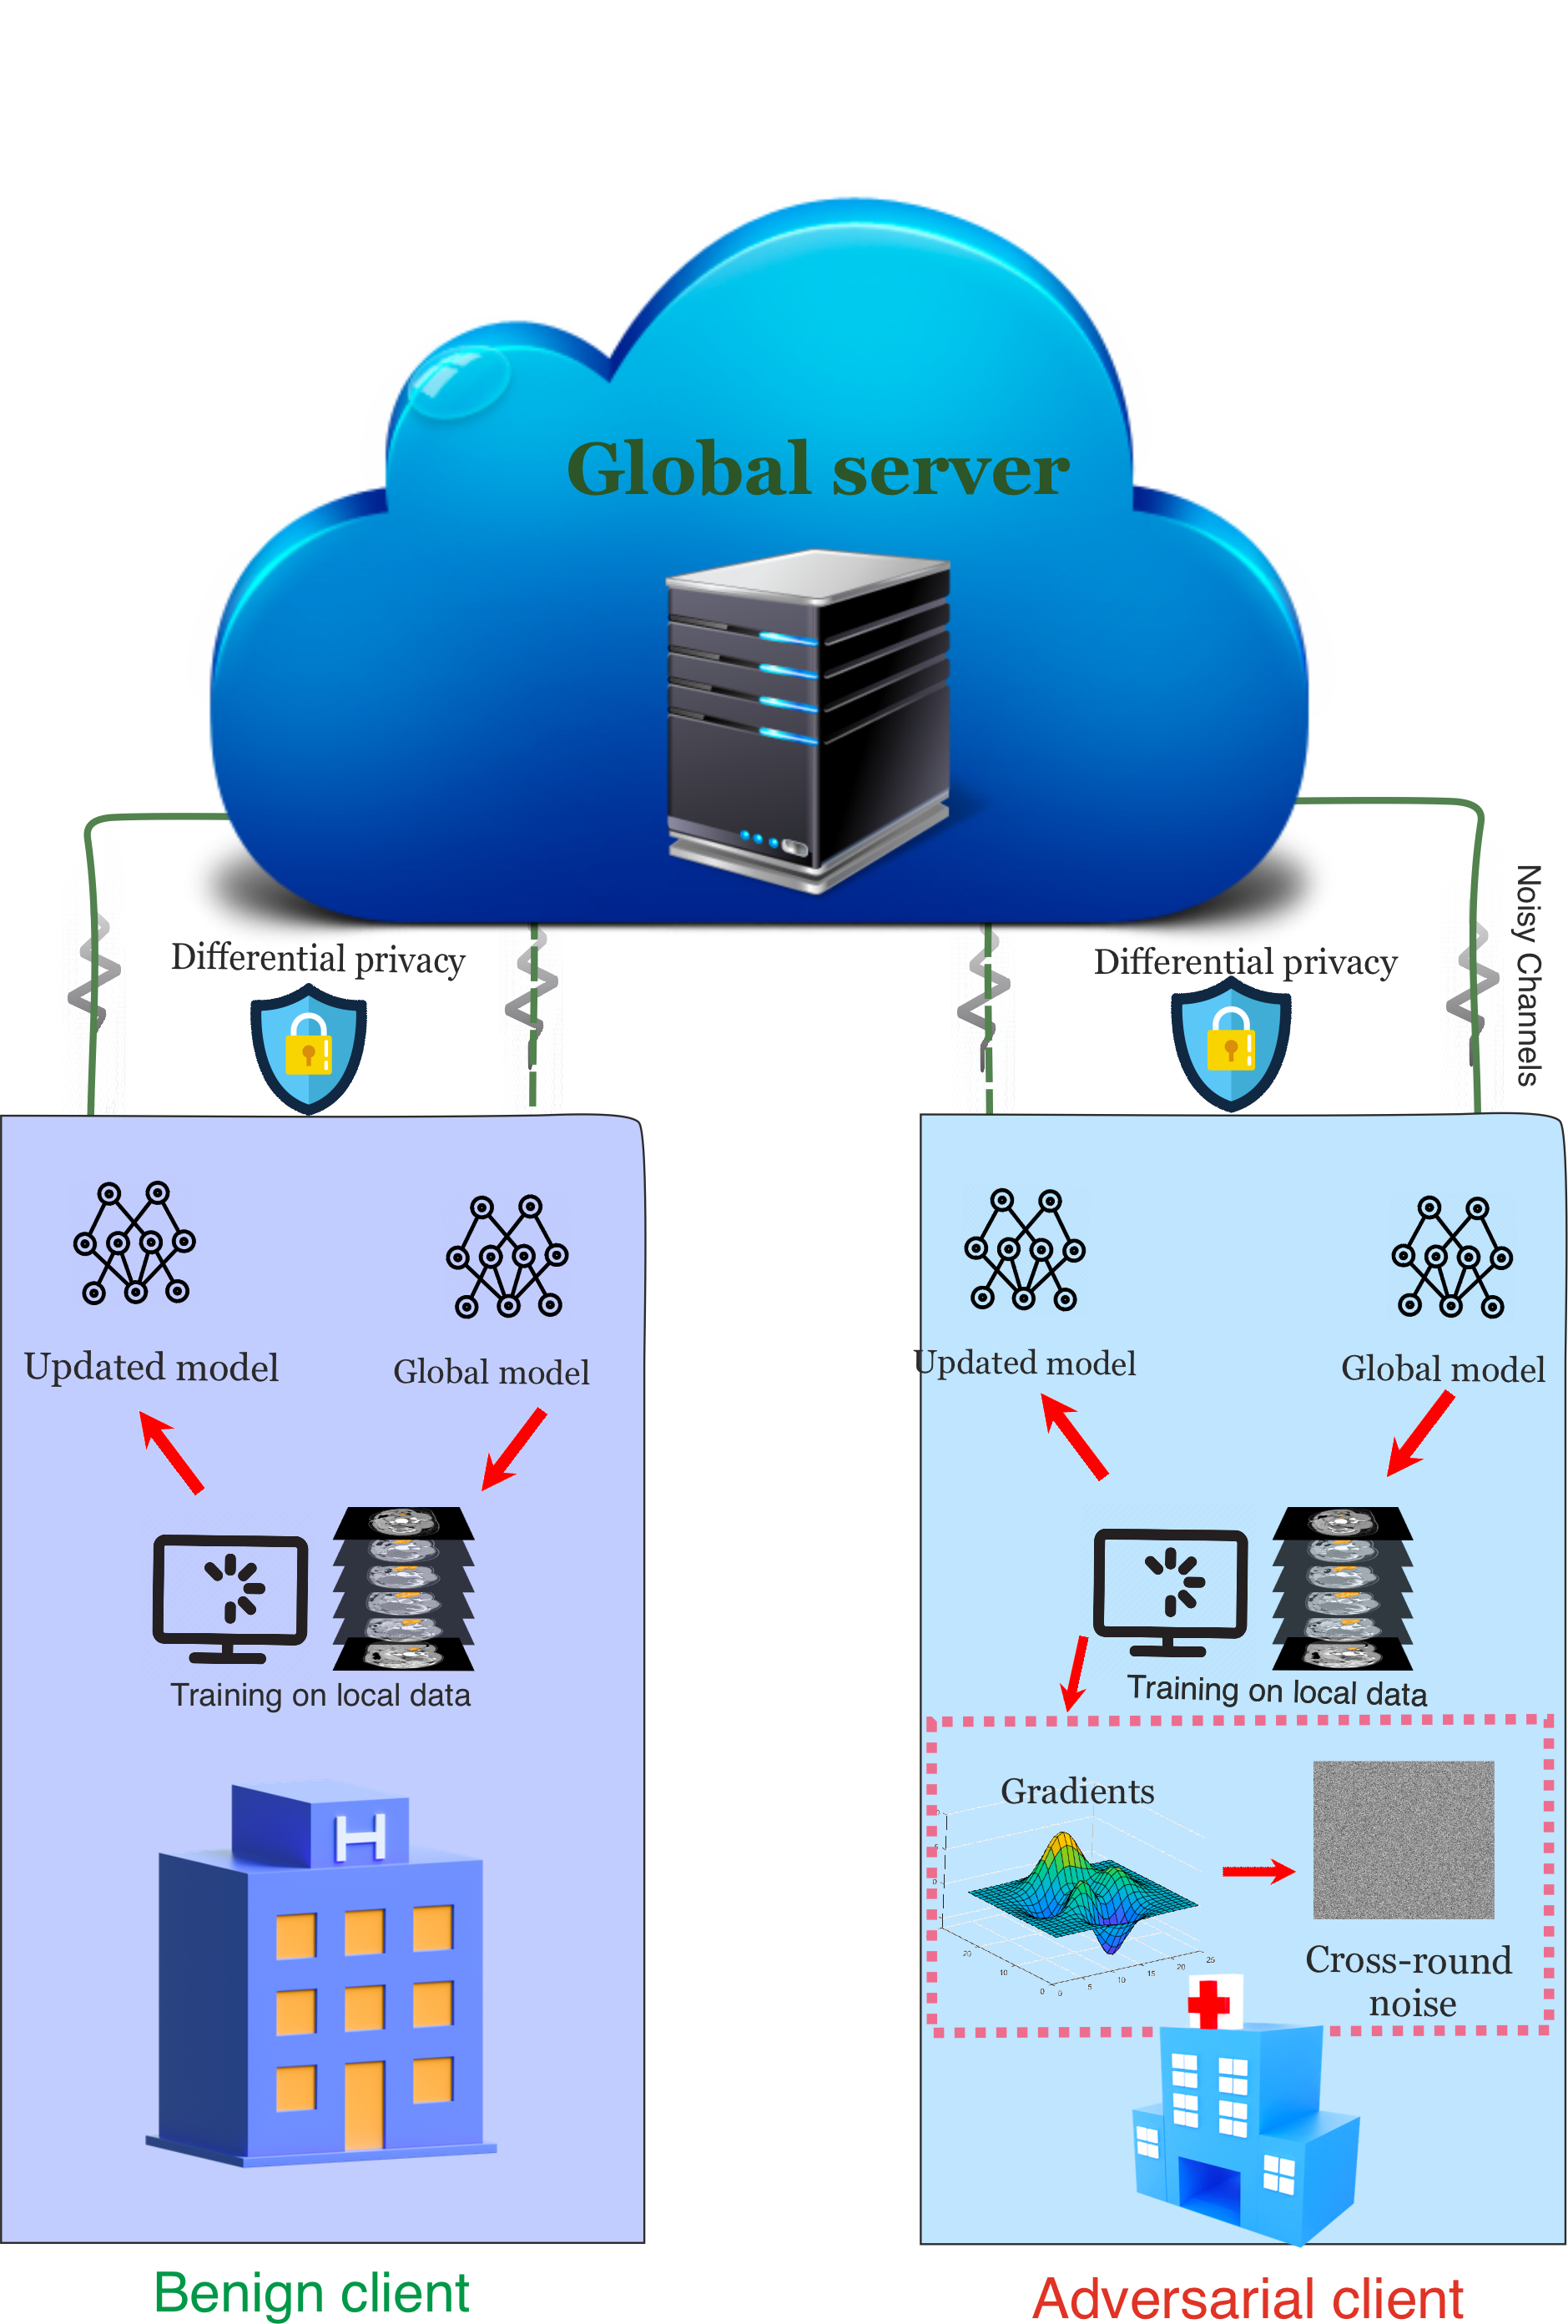
\includegraphics[width=0.50\textwidth]{Adversarialattacks.png}
%  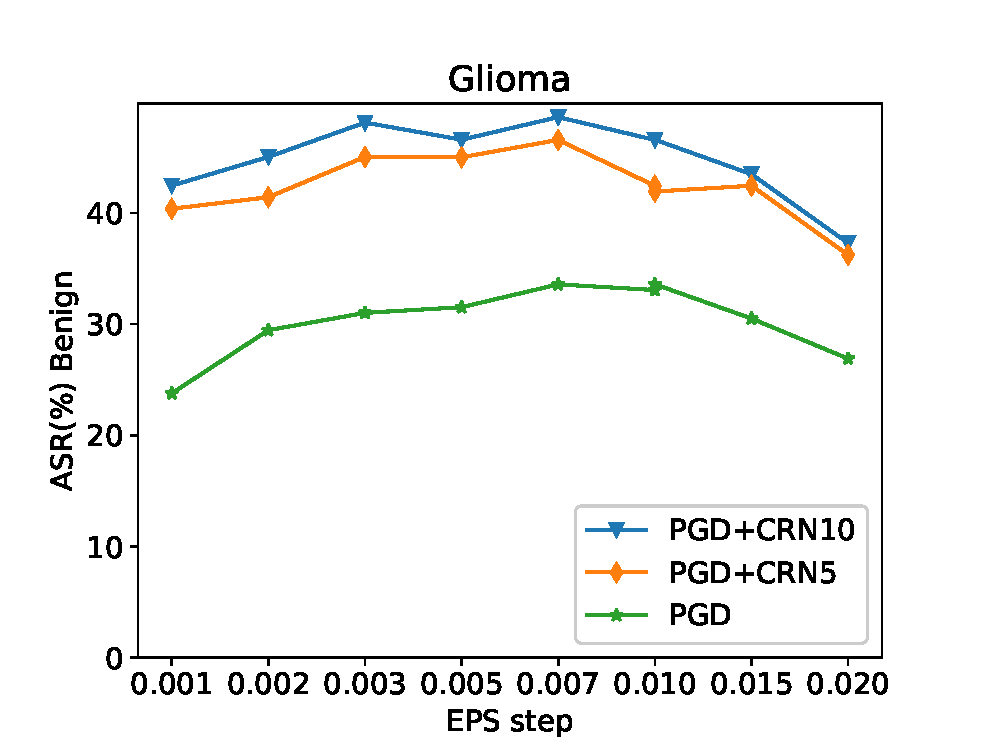
\includegraphics[width=0.50\textwidth]{Glioma_ASR_EPS_steps}
%  \caption{A schema of our method, at each FL round, the adversary transforms the gradients into cross-round noise, while acting as a benign client and not tampering the training process}
%  \label{fig:pgd-atta-comparison}
% \end{figure}


\begin{figure}[t!]
 \centering
 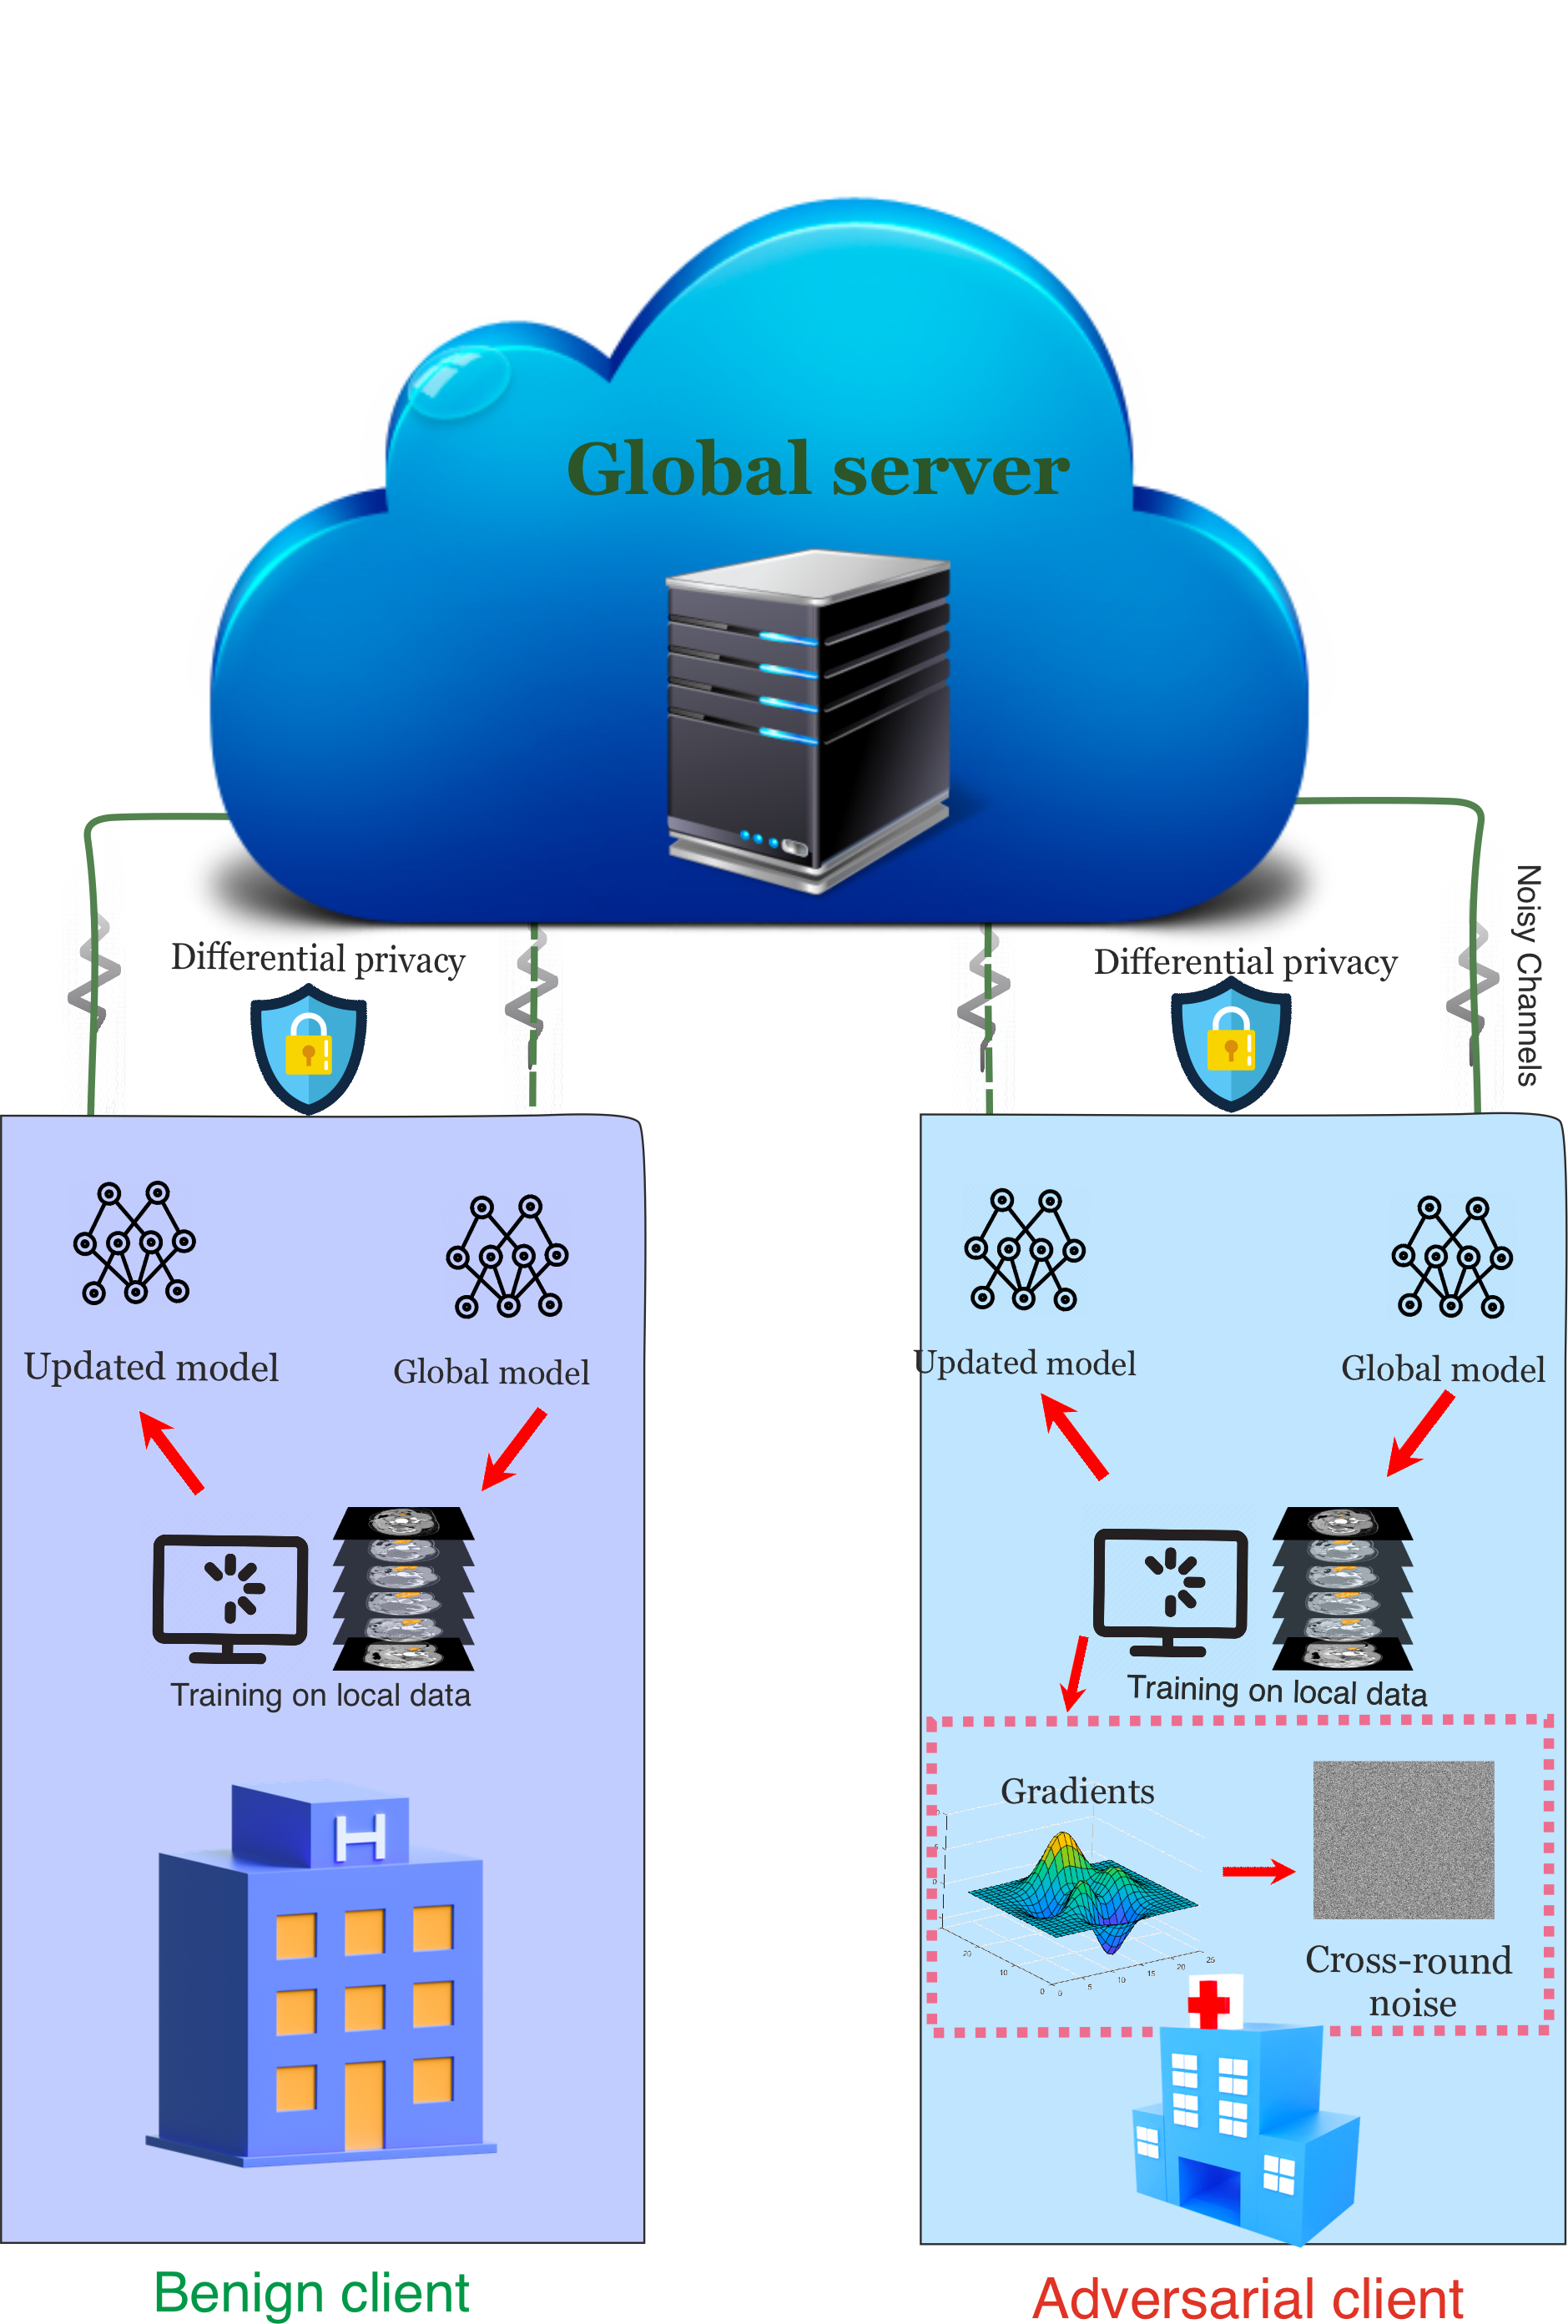
\includegraphics[width=0.50\textwidth]{Adversarialattacks.png}
 \caption{A schema of our method, at each FL round, the adversary transforms the gradients into cross-round noise, while acting as a benign client and not tampering the training process}
 \label{fig:pgd-atta-comparison}
\end{figure}

\subsection{Attack models}
Numerous adversarial attacks have been proposed by the literature in order to fool deep neural networks and produce false predictions. Adversarial attacks work through injecting a guided imperceptible noise that fools the trained deep learning model. Popular attack methods are Projected Gradient Descent (PGD), Fast Gradient Sign Method (FGSM, and Basic Iterative Method (BIM. Each will be discussed in this section.

\textbf{FGSM:} Fast Gradient Sign Method (FGSM) \cite{szegedy2013intriguing}is a fast yet effective method which produces adversary image with one step of calculation. Assuming input $x$ and its corresponding target $t$, FGSM calculates gradient of $x$ w.r.t the loss function ${\partial \mathcal{L}}/ \partial {x}$.

\begin{equation}
\label{eqt:fgsm}
    \bm{\hat{x}} = \bm{x} + \epsilon \cdot sgn\big(\nabla_{\bm{x}}{\mathcal{L}}(g(\bm{x};w)\big)
\end{equation}

where epsilon $\epsilon$ is a hyper-parameter which determines adversarial noise level. $g(\bm{x};\bm{w})$ is the output of neural network with respect to the input $x$ and parameter set $w$. $sgn(.)$ is the sign function. The result of sign function goes through a clipping function to impose a maximum bound in change to the perturbation $\epsilon \cdot sgn\big(\nabla_{\bm{x}}{\mathcal{L}}(g(\bm{x};\bm{w})\big)\in [-1,1]$.

\textbf{BIM:}  Basic Iterative Method (BIM) is an extension of the FGSM method, By Kurakin et al.\cite{kurakin2018adversarial} repeatedly do the process in FGSM, using a small step-size and $\bm{\hat{x}^{1}} = \bm{x}$. BIM is stronger than FGSM and requires smaller perturbations.

\textbf{PGD:} Madry et al. \cite{madry2017towards}proposed their own version of the BIM attack. In Projected Gradient Descent (PGD) \cite{madry2018towards}
the attack starts with a uniform random initialization. The update formula for PGD attack can be written as: 
\begin{equation}
\label{eqt:pgd}
    \bm{\hat{x}}^{t+1}=\Pi_{P_\epsilon(\bm{x})} \Big( \bm{\hat{x}}^t + \alpha \cdot sgn\big(\nabla_{\bm{x}}{\mathcal{L}}(g(\bm{\hat{x}}^t;\bm{w}),t)\big)\Big)
\end{equation}
Where $\bm{\hat{x}}^{k}$ is the perturbed data in $k$-th iteration, and $P_\epsilon(\bm{x})$ is the projected gradient descent function, which is done by first finding sign values, and then projecting the result to a small neighborhoud of the input ${x}$. This possible parameter spaces determines the set PGD attack samples that an adverdsary can use. PGD is one of the strongest attacks and is a universal first-order adversarial method. Technically, aside from formulazing the problem as projected gradient, PGD is similar to BIM but with random small initialization. We report results with PGD. With same number of iterations, BIM had the same results, or the difference was negligilbe.
	
% \subsection{Optional}
% blackbox/wihtebox
\section{Enhanced adversarial attack }
\label{sec:ourattack}
In this section we introduce our method to enhance the existing adversarial attacks in an FL setting.

\subsection{Threat model}


% \begin{algorithm}[th]
%  \caption{Adversarial Training with Transferable Adversarial Examples (ATTA)}\label{alg:atta}
%  \begin{algorithmic}[1]
%  \State \textbf{Input}: Padded training dataset $D_{nat}$, model $f_\theta$, attack algorithm $\mathcal{A}$, perturbation bound $\epsilon$, the number of epochs to reset perturbation $reset$
%  \State Initialize $\theta$
%  \State Initialize $D$ by cloning $D_{nat}$
%  \For{$epoch = 1 \cdots N$}
%  \For{$x_{nat},y$ in $D_{nat}$ and corresponding $x \in D$}
%  \If {$epoch\ \%\ reset\ =\ 0$}
%  \State $\beta \gets$ a small random perturbation
%  \State $x \gets x_{nat} + \beta$
%  \EndIf
%  \State Store the transformation $T_{aug}$ for the inverse augmentation:
%  \State $x_{aug}, x_{nat, aug}, T_{aug} \gets \dataaug(x, x_{adv})$
%  \State $x^* \gets \mathcal{A}(f_{\theta}, x_{nat, aug}, y, x_{aug}, \epsilon)$
%  \State $\theta \gets \theta - \nabla_{f_{\theta}} \frac{\partial \mathcal{L}(f_\theta, x^*, y)}{\partial \theta}$
%  \State $x \gets \inverseaug(x, x^*, T_{aug})$
%  \EndFor
%  \EndFor
%  \end{algorithmic}

% \end{algorithm}




We consider a scenario in which one FL participant is malicious or is controlled by a hostile adversary. The adversary tries to fool the global model by generating images similar to its real data.
We assume that the central server is honest and trusted.\\\textbf{Goal of adversary:}
The adversary's Goal is to manipulate the global model so that the global model has a higher classification error.  \\
\textbf{Knowledge of adversary:}
In a realistic scenario, the malicious party only can see its own data $D_{i}$, and knows the DNN architecture and the global model weights that it receives each round. \\
\textbf{Capability of adversary:}
No special privilege or Capability is assumed for the adversary. Similar to other clients, the adversary has control over its own training procedure and data, and it can not manipulate other clients' data or the general learning process. (e.g., local computations, communication with central server and aggregation process, DNN architecture, and optimization functions). It can interact with the model, query the outputs, and calculate the gradients. The adversary doesn't use the training data.




\subsection{Cross-round noise}



Adversarial examples being developed in the inference time, the adversary might not have the necessary computing power as they have during the training time. Also, sometimes inference is being done on third-party applications on edge devices where they don't have GPUs.
This might be crucial for the adversary, that it can prepare the attack samples with less computations. Iterative methods, such as PGD, require too much computational power to develop the examples. even more than normal training itself. \cite{zhang2019you} The problem could be worse for high-resolution or whole-slide images.
Also, PGD needs the target and surrogate to be highly similar to ensure transferability. However, models being noisy causes high inter-client variability, as a protection measure.

% Federetaed environemtn can introduce new surfaces to enhance adversarial transferability.  Gather more information about other clients by utilizing  global model upates.\cite{lyu2020threats}


% \begin{figure}[htbp!]
%  \centering
%  \includegraphics[width=0.10\textwidth]{Adversarial0attacks-7.eps}
%  \caption{Traditional adversarial training (PGD-$k$) (a) and ATTA-$k$ (b). $C$ is the connection function which improves the transferability between epochs.}
%  \label{fig:pgd-atta-comparison}
% \end{figure}
Incorporating prior knowledge already available from the global model, the attack can be initialized from a proper baseline so the computation might be reduced. Also, it might diminish the bias and lead to a broader estimation of other clients.



We introduce an intermediary noise tensor we call \textit{Cross-round noise} which extracts features from received global and is calculated alongside local epochs. The noise gets updated and passed to the next FL round. 
We use a function for the adversary to produce a noise based on ${L}_{2}$ regularized gradients at each FL training round. Then in the test phase, we use the noise to initialize the values for adversarial attack algorithms. 



\begin{algorithm}[t!]
\caption{Training procedure}
\label{alg:NbAFL}
\LinesNumbered
\KwData{$T$, $\beta$, ${w}^{(0)}$, $\mu$, $\epsilon$ and $\delta$}
{Initializing parameters: $t = 1$ and ${w}^{(0)}_{i} = {w}^{(0)}$ and ${{\mathcal{\delta}}^{(t)}=0}$} $\forall i,t$\\
\While {$t \le T$}
{
\textbf{Local training:}\\
\While {$\mathcal C_i\in \{\mathcal C_1, \mathcal C_2, \ldots,\mathcal C_{N}\}$}
{
Clients update their models ${w}^{(t)}_{i}$ as\\
% \quad\quad ${w}^{(t)}_{i}=\arg\min\limits_{{w}_{i}}{\left(F_{i}({w}_{i})+\frac{\mu}{2}\Vert {w}_{i}-
\quad${w}^{(t)}_{i}=\arg\min\limits_{{w}_{i}}{\left(\mathcal{L}_{i}({w}_{i})\right)}$\\
Clients clip parameters ${w}^{(t)}_{i} = {w}^{(t)}_{i}/\max\left(1,\frac{\Vert{w}^{(t)}_{i}\Vert}{C}\right)$\\
Clients add Gaussian noise\\ $\widetilde{{w}}^{(t)}_{i}={w}^{(t)}_{i}+{n}^{(t)}_{i}$\\
}
\textbf{Global update:}\\
Global server individual models ${w}^{(t)}$ as\\
\quad\quad ${w}^{(t)} = \sum\limits_{i=1}^{N}{p_{i}\widetilde{{w}}^{(t)}_{i}}$\\
Global server adds Gaussian noise \\
\quad\quad$\widetilde{{w}_{i}}^{(t)}={w}^{(t)}+{n}_{\text i}^{(t)}$\\
\If{$t \ge \beta$}
    {
% \textbf{Adversairal client:}\\
  \textbf{Adversarial client} $\mathcal C_{m},   \mathcal X \in \mathcal D_m:$
  % ,  {\mathcal{\delta}^{(\beta)}=0,$:}\\
% \quad\quad
\\Adversary performs gradient regularization \\
\quad{${{\nabla_{\mathcal{X}}\mathcal{\hat{L}}\gets \nabla_{\mathcal{X}}\mathcal{L}(\mathcal {\delta}^{(t-1)},\widetilde{{w}_{m}}^{(t)}})}$}\\
% ${\mathcal{\delta}}^{(t)}\gets \epsilon . sgn(\nabla_{\mathcal{X}}\mathcal{\hat{L}}(\mathcal {\delta}^{(t-1)},\mathcal{X},\widetilde{{w}_{m}}^{(t)})$
% \quad\quad${{\mathcal{\delta}}^{(t)}\gets \epsilon . sgn(\nabla_{\mathcal{X}}\mathcal{\hat{L}}(\mathcal {\delta}^{(t-1)},\widetilde{{w}_{m}}^{(t)}}))$
\\Adversary projects the gradient \\

\quad$\mathcal{\delta}^{(t)}\gets \Pi_{P_\epsilon(\bm{0})}(\nabla_{\mathcal{X}}\mathcal{\hat{L})}$
}
% Test the received parameters $\widetilde{\mathbf{w_{i}}}^{(t)}$ using local dataset\\
% 
\\$t\leftarrow t + 1$}
% #2ndPart#########################
% #2nd Part#########################
% #2nd Part#########################
% #2nd Part#########################
% #2nd Part#########################
% #2nd Part#########################
% #2nd Part#########################
% #2nd Part#########################
% #2nd Part#########################}
% \textbf{Adversarial attack process:}\\
% % {Initialization: $\mathcal$ and ${w}^{(0)}_{i} = {w}^{(0)}$} 
% {\While \{$\mathcal C_i\in \{\mathcal C_1, \mathcal C_2, \ldots,\mathcal C_{N}\}$}
% { 
% Update the local parameters ${w}^{(t)}_{i}$ as\\
% % \quad\quad ${w}^{(t)}_{i}=\arg\min\limits_{{w}_{i}}{\left(F_{i}({w}_{i})+\frac{\mu}{2}\Vert {w}_{i}-}
% }
% % Test the receivedparameters $\widetilde{\mathbf{w_{i}}}^{(t)}$ using local dataset\\
% $t\leftarrow t + 1$}}}
% % \KwResult{$\widetilde{{w}}^{(T)},{\mathbf{\mathcal{{\delta}}}^{T}}$}}
\KwResult{$\widetilde{{w}_{i}}^{(T)},{\mathbf{\mathcal{{\delta}}}^{T}}$}
\end{algorithm}

\subsubsection{Gradient calculation}


The noise is calculated by the gradients of model at each round. The adversary uses the loss:

% \begin{equation}
% \label{eqt:loss}
% L(f_{r}({x}_{adv},f_{r}{(x))})
% \end{equation}


\begin{equation}
\label{eqt:loss1}
 \nabla_{\bm{x}}{\mathcal{L}}(g(\bm{x+\delta}^{(t)};\bm{w^{(t)}}),g(\bm{x};\bm{w^{(t)}}))
\end{equation}
% \hl{BIM/ PGD ro yejuri joda kon}
To update the stored values for the noise. In which $g(.;\theta^{t})$ refers to received global model in communication round $t$.  The adversary iteratively updates the noise by maximizing the loss between the model output for the noisy and the clean test data. 
% Here we assumed that the adversary does not have access to the labels. So the true labels are not used for the loss function. 
% \hl{mituni bahs koni chera in behtar az ine ke loss ro nesbat be label hesab konim}. 
The global model parameters change for the test dataset being the same in each round. 
\cite{zhang2019theoretically}
Saving noise could be started after an arbitrary number of rounds is passed, say, $\beta$ and be calculated alongside local training with similar epochs. In this paper, we consider initializing from the last 10 and last 5 rounds. Calling them CRN10 and CRN5 respectively.
% This process can also be done for several iterations, depending on the value of $\epsilon$.
% \hl{$\beta$ ro  .iar too bahs}
\\\subsubsection{$L_{2}$ regularization}

Transferring gradient information between models might lead to drastic parameter change.\cite{zhang2019theoretically,pan2019improving,dettmers20158}. Unlike some methods which manually reset the gradients, so they lose information \cite{zheng2020efficient}, we regularize the change in CRN by subtracting the mean value in each channel of the input noise. We apply a function for $L_{2}$ regularization the gradients.
\begin{equation}
    \nabla_{x_{i}}\mathcal{\hat{L}} = \nabla_{x_{i}}\mathcal{{L}} -  \frac{1}{M} \sum\limits_{j=1}^{M}{\nabla_{x}_{_{i,j}}} \mathcal{{L}}
\end{equation}
The resulting value is channel-wise regularized loss, and $i$ indicates index of channel, and $j$ refers to individual pixels. This results in a smaller $L_{2}$ norm of gradient values, which is a proven measure against explosion or outlier gradients. \cite{pascanu2013difficulty}\cite{kim2016accurate} . 
\\Then it goes through projection procedure, which the final values are $L_\infty$ bounded around zero, with a small value $\epsilon$. 
% To ensure the noise stays sufficiently small 


\subsection{Inference phase attack}
Attacks are performed after training is done. FGSM and BIM use zero initialization, and PGD uses random initialization, then they compute the adversarial example according to Equations \ref{eqt:fgsm} and \ref{eqt:pgd}.\\
We use the cross-round noise added to the input test data as an initial point for these methods, \\



showing that they can improve substantially.\\ Adversarial examples can be computed even with one step of computation, and non-iterative models like FGSM can be strong enough to outperform PGD with random initialization.\\
These iterative algorithms put lots of loads since the projected gradient descent is very expensive to compute. \cite{shafahi2019adversarial}
It is possible that models are integrated into another environment like PACS or software. Training these models is time-consuming and might be a burden.




\section{Experiment}




\subsection{Datasets}

\textbf{Brain cancer classification:}Dataset for detecting brain cancer is downloaded from Kaggle. It contains brain MRI images categorized into four classes: Three types of brain tumor,  and one healthy no Tumor class. 
% For tumor type classification task, 2870 images for training and 394 images for the test. 
For Meningioma and Glioma detection, 1437 and 1426 samples were used, respectively,  and they were split as train/ test data. Transforms rotation, Flipping, and normalizing.  Images were resized to 100$\times$100. 
\\
\textbf{Histopathologic cancer detection:} 
The samples are metastasic tissue images of lymph node cancer. Images are in size ,96 $\times$ 96, and the task is to classify the tissue samples. Each positive sample has a metastasic region, which is located in $32\times32$ neighborhood of each image sample. 
% Tumor tissue in the outer region of the patch does not influence the label. 
They were categorized into cancer and non-cancer classes. 2150 samples were chosen and randomly assigned to clients, and each split 62\% for train and 38\% for the test. We used horizontal Flipping, and images were normalized.

% \\\hl{A ro tu line 21 algorithm taarif kon va dorost kon notionesh ro}
\subsection{Network architectures}

\textbf{Deep learning models:}
The deep learning model used is a Convolutional Neural Network (CNN) with six layers of convolution stacked to 5 fully connected layers. The activation function used is ReLU. And dropout parameter (0.25). The last layer depends on the number of classes (4 or 2). Models are all trained and converged before implementing adversarial attacks.
They are trained with Cross-Entropy loss and with an SGD optimizer. Four models are trained separately. Two binary classification models are trained to detect Meningioma and Glioma from the healthy No Tumor class. One model is trained to detect cancer in HistoPathology images.

\textbf{Federated setting:}
Three clients are defined for the FL setup. The data is assigned randomly, and the clients have non-IID data distribution.
The FedAVG method is used to aggregate the models. The aggregation is weighed based on the length of the training dataset. Each client is trained for 20 epochs at the communication round. The total FL rounds are 50.

\subsection{Attack setting}

Each client is assigned 100 test samples to perform the adversarial attack. Each client is selected as the adversary, and the results are averaged at the end. 
% The attacks are conducted with different $\epsilon$ and gradient steps $\alpha$ to evaluate the effect on the final result. 
We use three metrics,
Clean accuracy is defined as the performance of models on uncorrupted test images, \textit{Attack Success Rate (ASR)}; how much an adversary can change the predicted labels produced by each model, \textit{Average Error Transferability Rate (AETR)} to evaluate transferability. An adversary might propose an attack by only selecting the samples that successfully fooled its own model. AETR measures how successfully these samples changed the target models' correct predictions. So unlike ASR, this metric doesn't count the examples that were initially misclassified by the victim model.\cite{papernot2017practical},

\begin{figure*}[h!]
     \centering
     \begin{subfigure}
         \centering
         \includegraphics[width=0.32\textwidth]{Meningioma_ASR_EPS.eps}
          \includegraphics[width=0.32\textwidth]{Glioma_ASR_EPS.eps}
           \includegraphics[width=0.32\textwidth]{Pathology_ASR_EPS.eps}
         \caption{Effect of $\epsilon$ on Average ASR on benign clients }
         \label{fig:AASR benign-EPS}
     \end{subfigure}
     \hfill
     \begin{subfigure}
          \centering
         \includegraphics[width=0.32\textwidth]{Meningioma_others_EPS.eps}
          \includegraphics[width=0.32\textwidth]{Glioma_others_EPS.eps}
           \includegraphics[width=0.32\textwidth]{Pathology_others_EPS.eps}
         \caption{Effect of $\epsilon$ on ASR on the advesarial client }
         \label{fig:AASR malignant-EPS}
     \end{subfigure}
     \hfill
        \caption{Effect of Error perturbation degree $\epsilon$ on attack transferability. FGSM and PGD attack with and without CRN initialization where performed. CRN initalizations used 10 models and another one loading 5.  ASR is calculated on benign and adversary clients. The results of with varying perturbation degrees. The higher ASR on benign clients shows higher transferability}
        \label{fig: epsilon graphs}
\end{figure*}

  Here, we expand the previous findings to the FL settings and discuss whether change in $\epsilon$ can lead to transferability. 
  
We perform three analysis to find important factors in attack success:
\begin{itemize}
    \item We investigate dependency of attacker on $\epsilon$. By visual inspection and ASR evaluation, and as a comparison to previously found optimal known values in centralized  setting.
    \item  We compare  efficiency of models, by discussing their attack preparation time and their ASR.
    \item We also see how attack step $\alpha$ can determine ASR.
\end{itemize}



\section{Results}







% Original images, adversarial images, and corresponding adversarial noise created with FGSM ( ϵ=0.02) in different black-box settings


\subsection{Efficiency analysis}


\begin{figure*}[h!]
     \centering
     \begin{subfigure}
         \centering
         \includegraphics[width=0.32\textwidth]{Meningioma_ASR_EPS_steps.eps}
          \includegraphics[width=0.32\textwidth]{Glioma_ASR_EPS_steps.eps}
           \includegraphics[width=0.32\textwidth]{Pathology_ASR_EPS_steps.eps}
         \caption{Average ASR on benign clients }
         \label{fig:y equals x}
     \end{subfigure}
     \hfill
     \begin{subfigure}
          \centering
         \includegraphics[width=0.32\textwidth]{Meningioma_others_EPS_steps.eps}
          \includegraphics[width=0.32\textwidth]{Glioma_others_EPS_steps.eps}
           \includegraphics[width=0.32\textwidth]{Pathology_others_EPS_steps.eps}
         \caption{Average ASR on advesarial client }
         \label{fig:y equals x}
     \end{subfigure}
     \hfill
        \caption{Effect of Error perturbation step $\alpha$ on attack transferability. PGD attack with CRN initalizations used 10 models and another one loading 5. ASR is calculated on benign and adversary clients. The results of with varying perturbation steps. The higher ASR on benign clients shows higher transferability}
        \label{fig:three graphs}
\end{figure*}

The models are trained in an FL enviroment. Average test results, or clean accuracy shows the average performance of clients on unperturbed test data. This could be a baseline for comparison of attacks.
Here we compare the computational complexity of iterative algorithms. The comparison is based on the time required to train one batch of adversarial examples, with  $\epsilon=0.05$ and $\alpha=0.001$. The average Attack success rate is the average of ASR for all test samples of all clients and indicates the transferability in the FL network.
As expected \ref{table_time}, the higher iteration rounds take more computation and lead to higher AASR. Generally, computational complexity has a linear dependence on the number of iterations. However, the increase in transferability can vary. If PGD performs poorly initially, having higher iterations doesn't help much. 

Also, CRN does not require additional computation. Similar to single-step methods, computational load is small but increases on high-resolution images. As an example, the pathology dataset requires more calculation than MRI data. 
However, the overall time is far less than iterative models, and also it could enhance the transferability much better. The effect is consistent among different datasets. 
% However,  This means that Pathology images have better AASR than MRI images in baseline and CRN enabled attacks.
% Also,  

% PGD can sometimes perform poorly, even in higher iterations. Enabling the initialization might  


\begin{table}[h!]
\centering
\setlength{\tabcolsep}{6pt}
\renewcommand\arraystretch{1.22}
\caption{ \small Comparison of iterative models and their copmutational efficiency, on performing computations on one batch of data.  ACC shows average client performance for unperturbed test data. AASR is average ASR on all clients.}
\begin{tabular}{| *{5}{c|} }
\hline
Dataset  & Attack type & ACC & AASR & time (sec)
\\   \hline  
\multirow{3}{5em}{Meningioma}     &\textbf{PGD-1+CRN10}&\multirow{3}{3em}{84.12\%}&\textbf{63.92\%} & \textbf{0.217}  \\
 &PGD-20&&27.52\% & 3.423 \\
&PGD-40&&32.99\% & 6.794  \\ \hline
\multirow{3}{4em}{Pathology}     &\textbf{PGD-1+CRN10}&\multirow{3}{3em}{77.01\%}&\textbf{90.92\%} & \textbf{0.354} \\
&PGD-20&&60.98\% & 5.464\\
&PGD-40&&82.27\% & 10.843 \\ \hline
\multirow{3}{3em}{Glioma}     &\textbf{PGD-1+CRN10}&\multirow{3}{3em}{61.84\%}&\textbf{70.55}\% & \textbf{0.216}  \\
&PGD-20&&51.83\% &3.420  \\
&PGD-40&&63.77\% & 6.793  \\ \hline


\end{tabular}
\label{table_time} 
\end{table}




\subsection{Effect perturbation degree}

We performed attack scenarios to evaluate the effect of perturbation degree $\epsilon$  on attack success on the model. We compared the baseline attack to CRN- enabled attacks. ASR is calculated on benign and adversary clients and is shown in Fig \ref{fig: epsilon graphs}.

More successful attacks on adversaries led to higher transferability to benign clients. Low values of $\epsilon$ can decrease transferability to a large extent. $\epsilon$ = 0.01 has poor performance on all the clients. Generally, Higher $\epsilon$ values lead to higher ASR in all scenarios. Although for Meningioma and Glioma images, increasing $\epsilon$ from 0.04 didn't have much positive effect in PGD and FGSM methods on the adversarial client. 
In pathology images, Iterative models can reach perfect accuracy on the adversarial client and have very high transferability.

CRN  has a positive effect on transferability in all scenarios. Also, CRN-enabled models are more dependent on $\epsilon$; their extent can vary depending on the dataset, attack method, and value of $\epsilon$.
Tuning $\epsilon$  might be tricky since performance and imperceptibility should be considered together.High $\epsilon$ values mean more distortion in the image. We performed an FGSM attack with varying $\epsilon$ values to evaluate the perturbation effect visually. Fig \ref{fig:perturbedMRI} shows the results of perturbed images with different perturbation degrees and their comparison with the unperturbed image. Note that perturbation values below  $\epsilon=0.05$ cause limited distortion.


Iterative models can reach high ASR very quickly with increasing $\epsilon$. 

\begin{figure*}[h!]
 \centering
 \includegraphics[width=0.8\textwidth]{Adversarial_attacks-5.eps}
 \caption{\small From (a) to (f), normal tumor image, and petrurbed images with FGSM attack, with perturbation parameters: $\epsilon$ = 0.01, 0.03, 0.05,  0.10, respectively}
 \label{fig:perturbedMRI}
\end{figure*}











% \subsection{AATR}
% \begin{table}[h]
% \centering
% \setlength{\tabcolsep}{8pt}
% \renewcommand\arraystretch{1.4}
% \caption{Result of our experiments for PGD attack on Pathology data $\epsilon$ values. The iterative models are trained for 40 rounds with step size of 0.01. \hl{\faQuestion maybe you can change the word for without CRN}}
% % \begin{tabular}{cccccccccccc}
% \begin{tabular}{| *{4}{c|} }\hline
% % Dataset  & Attack type & \multicolumn{2}{c|}{ $\epsilon=0.01$} & \multicolumn{2}{c|}{ $\epsilon=0.03$}           &    \multicolumn{2}{c|}{ $\epsilon=0.05$}    & \multicolumn{2}{c|}{ $\epsilon=0.07$}                                                              \\ \hline
%  Dataset&\multicolumn{3}{c|}{ FGSM}    
% %  &              \multicolumn{3}{c|}{ PGD}                                                                           \\  

%  \cline{2-5}
% &Baseline&CRN5 &CRN10\\\hline

% Meningioma&84.80\%&\textbf{86.31}\%&{84.02\%}
% % \%&83.73\%  &\textbf{84.25}\%  &84.16\%
% \\\hline
% Glioma&82.32\% &87.06\%&\textbf{89.98\%}
% % &74.89\%&\textbf{83.64}\% &82.32\%
% \\\hline

% Pathology&\textbf{90.67\%}&{84.81\%}\%&{85.98\%}
% % \%&79.86\% &86.79\%&\textbf{86.93\%}
% \\\hline



% \end{tabular}
% \label{table_core} 
% \end{table}










\subsection{Effect perturbation step}


Another critical parameter is the step of change in iterative methods. {$\alpha$} is shown to be highly deterministic in specific settings, but is not yet investigated in MIA domain. To evaluate how $\alpha$ can affect transferability, we examined the clients with $\eps=0.03$. Under various steps. The general observation is that there is an optimal middle range the same as $\epsilon$. The step size of 0.007 led to the highest transferability in MRI images. Larger steps led to a sharp decrease in transferability. For pathology images, midspans, about 0.007 led to the best ASR on the adversary, and higher values decreased both ASR on adversary and transferability. However, smaller steps also had high ASR values. 







\subsection{Error tranferability}




Another measure is the average error transfer rate (AETR). Although PGD outperforms FGSM in ASR, in AETR, the results are close. PGD is trained for 40 iterations, and the models are compared with and without CRN.
Both FGSM and PGD having high AETR suggest that although FGSM might not be able to produce high-quality samples in general, the good examples which can fool the adversary are also highly transferable to benign clients. And can be better than PGD samples. CRN generally increases the AETR. 




\begin{table*}[h!]
\centering
\setlength{\tabcolsep}{8pt}
\renewcommand\arraystretch{1.4}
\caption{Result of Average Error Transfer Rate (AETR) for FGSM and PGD methods, with and without CRN initalization }
% \begin{tabular}{cccccccccccc}
\begin{tabular}{| *{7}{c|} }\hline
% Dataset  & Attack type & \multicolumn{2}{c|}{ $\epsilon=0.01$} & \multicolumn{2}{c|}{ $\epsilon=0.03$}           &    \multicolumn{2}{c|}{ $\epsilon=0.05$}    & \multicolumn{2}{c|}{ $\epsilon=0.07$}                                                              \\ \hline
 Dataset&\multicolumn{3}{c|}{ FGSM}     &              \multicolumn{3}{c|}{ PGD}                                                                           \\  

 \cline{2-7}
&Baseline&CRN5 &CRN10&Baeline&CRN5&CRN10\\\hline

Meningioma&84.80\%&\textbf{86.31}\%&{84.02}\%&83.73\%  &\textbf{84.25}\%  &84.16\%\\\hline
Glioma&82.32\% &87.06&\textbf{89.98}&74.89\%&\textbf{83.64}\% &82.32\%\\\hline

Pathology&\textbf{90.67\%}&{84.81}\%&{85.98}\%&79.86\% &86.79\%&\textbf{86.93\%}\\\hline



\end{tabular}
\label{table_core} 
\end{table*}


% \newpage



\section{Discussion}

Our results admit the prior research about vulnerability of FL networks
\cite{goldblum2020dataset,liu2022threats,sun2019can,fang2020local,wang2020attack,song2020analyzing,wilkinson2016fair,van2022ai,miotto2016deep,costa2021covert,bouacida2021vulnerabilities} and MI systems 
 \cite{ma2021understanding,finlayson2019adversarial,gupta2022vulnerability,bortsova2021adversarial}  to adversaraial attacks.

% Our results suggest that even in a DP-enabled setting, adversarial samples generated on one client can be highly transferable.

We also found that differential privacy might have partial effect on attacker's success. In fact, DP caused the lower ASR in surrogate than the adversary clients.
% But it can not be considered as an effective counter-measure.
Although some research support DP, our findings suggest that more with ones who describe it as an option but not very reliable. \cite{bouacida2021vulnerabilities}. Also, the accuracy compromise coming with noise should be considered. \cite{canonne2020discrete} \cite{wang2019privacy}.
\\In our experiments the attacker did not tamper with the training procedure. his is unlike backdoor or poisoning attacks.\cite{lyu2020privacy}\cite{lyu2020threats}. where the attacker performs malicious activities during training, and opens the way for detection methods.
Also, CRN initialization led to faster attacks with higher transferability. This section discusses our findings, how they could be important in the MI domain, and what to consider when setting up FL MI infrastructure.



\subsection{Transferability}
% The practice could be that not always adding noise is better, especially in medical images where compromising accuracy affects patients. Other methods have their problems as stated before, \cite{yin2022adc,yuan2019adversarial,uesato2018adversarial} mainly compromising performance or working in certain conditions. 
% Further research might consider defense models of FL networks. 
Our experiments aimed to asses some factors in transferability. However, other than investigated factors, we found three other parameters might highly predict transferability.

\textbf{Benign/Adversary correlation:} Our results show that ASR on benign and adversary clients are highly correlated. Hence, for the adversary to ensure it can fool other clients in a black-box setting, it needs to obtain good results on its own data and model. So tuning the hyperparamets, data preprocessing can be all effective as long as they improve ASR on adversary.

\textbf{AETR/ASR difference:}, Attacks have higher AETR than ASR, which enables the adversary to subsample examples to achieve higher transferability. 
%. In black-box models, the attack results might vary from low transferability to similar to white-box. Depending on many parameters. But when implementing in a
% FL environment, the results are closer to the white-box setting. 
% This finding admits that models trained in FL setting keep their traditional ML vulnerabilities, and FL imposes an additional threat. Leading to aggregated vulnerabilty.\hl{  \faClockOshayad ye graph peyda Koni ke ASR ro ba white/black tozih bede}

\textbf{Attack domain}: We observed that transferability is specific within imaging domains, which is consistent with prior findings.\cite{bortsova2021adversarial} Attacks on Pathology images were consistently more successful than MRI images. 

% \subsection{Effect of parameters}
\textbf{Perturbation parameter}
% $\epsilon$  As shown in \ref{fig: epsilon graphs} 
Level of $\epsilon$ can substantially change transferability. Increasing $\epsilon$ does not improve ASR from a certain point, but adding CRN can increase the dependency. The best perturbation range in our experiments is around 0.03-0.05. These results suggest that conclusions in a centralized setting might not apply to an FL environment. And it shows different transferability behavior or parameter dependence.

\textbf{Step parameter } Our findings show that common $\alpha$ values have a  negligible effect on the final results, aside from too small or too large values. The reason could be that $\alpha$ similar to  $\epsilon$  bounds the change in each iteration, but generally, its values are one order of magnitude less than $\epsilon$. 


\subsection{Efficiency}
% Attacks can substantially differ in the computational requirements, 
% which can have practical implications in the MIA domain.
Our results show that initialization can be influential in computational efficiency. PGD with random intialization requires high computational power wihch migh be burdensome for High-resolution or large-batch training. Using CRN leads to much fewer computational requirements. Single-step attacks can be $20 \sim 30 \times$ less expensive than iterative models with 40 iterations and higher ASR. 
More minor GPU requirements \\Adversaries might be capable of attacks using high-volumes of data or with multiple devices by using CRN.
\\Standard ways of simulating attacks, like adaptive models and sanity checks, \cite{carlini2019evaluating} might be unfeasible in their traditional way. An adversary might have more knowledge than what is assumed in evaluation models, hence using more efficient methods or attacks with unexpected devices.



\subsection{Practical implications and suggestions}

In the following paragraphs, we discuss the motivations that cause adversarial attacks .

The large healthcare economy causes more benefit for malicious behavior, as there are existing reports of pervasive fraud in healthcare. Medical record manipulation for financial purposes \cite{ma2021understanding} fake trial reports\cite{george2015data} in radiology \cite{chowdhry2014image} and pathology\cite{suvarna2001histopathology} are widespread practices, and already made billions of dollars profit \cite{graese2016assessing} for fraudsters. Also, advanced fabrication algorithms and hard to detect methods are always intruguing for fradusters. Existing Manipulations like altering the visual features of images, or using photo editing software, \cite{chowdhry2014image} can result in images of benign subjects classified as malignant.\cite{xia2020pseudo}
\cite{sun2020adversarial}, but with visual distoration. In contrast, adversarial attacks are imperceptible, do not require manual intervention, and have high transferability. That gives a significant incentive for potential fraudsters to utilize adversarial attacks for high potential revenue. \\For example, consider a hypothetical case in which insurance companies utilize AI-based systems to approve a disease and get refund. A malicious person could add adversarial noise to images to manipulate insurance companies. Or consider if a person tries to bill insurance companies by reporting falsified surgical procedures. They can use attack algorithms to synthesize fake MRI and send it to the target company.
\\These vulnerabilities have some implications for clinical decision-makers, stakeholders, and insurance companies, who consider deploying FL or AI pipelines , which will be discussed in the following.
 
\begin{enumerate}[(i)]
    \item  First, they might take the pervasive motivation of manipulation and fraud into consideration, and beware of the financial and incentive \cite{finlayson2019adversarial}
    \item Second, having secure infrastructure in training phase does not guarantee safety in the deployment phase. So they might distinguish between these two, and consider redundant ways of incorporating AI in their MIA pipelines.
\item  Third, they might reconsider size and level of trust in collaborative/FL networks. Smaller networks with trusted parties have lower probability of having potential adversary.
\item Fourth, by not enforcing same data pre-processing pipelines, they might be able to hinder the adversary. They might also consider that having disparate data affects performance or even convergence of FL network.\cite{li2019convergence}. and how should they deal with the compromise between safety and performance.
\end{enumerate}

\\For developers of MIA systems these findings can have consider four things :

\begin{enumerate}[(i)]
    \item They can help end-users and clinicians by providing them more information other than model outputs. For example, adding explainable system reports helps the clinicians evaluate the legitimacy of predictions.
    \item Standard ways of evaluating robustness \cite{carlini2019evaluating}are not recommended in FL setting. so they might consider scenarios where adversary traces the global model, and has more knowledge, or attacks with unexpected devices.
    \item There is no universal factors to predict the capability of adversary, so they might consider existing research to important factor for each setting, or they might to a brute-force search to find upper-bounds of vulnerability. \cite{carlini2019evaluating} 
     \item Despite not having a universal defense method, there are limited case-specific defense models shown to work on some datasets, \cite{graese2016assessing} so developers might consider looking into potnetial defense method for their usecase.
\end{enumerate}





% One implication it might give is that, we might increase the robustness of FL network, 


\section{Conclusion}


This paper investigated adversarial attacks on federated MIA systems and discussed the crucial parameters on their transferability. We also proposed a new method that leverages the federated setting to improve the attack success rate and reduce the computation burden.
We saw that tuning the parameters can substantially improve transferability.
We also observed that adequately using noise from previous model updates can effectively improve computational load and has the potential to be well integrated into the existing attack methods.

Future lines of research could be to improve existing defense methods,\cite{sun2019can,wang2020attack,shao2019stochastic,li2019distributed,ma2019privacy,li2020multi ,yin2022adc,zheng2020efficient,yuan2019adversarial,uesato2018adversarial} , towards a universal defense algorithm. Another line of research could be how to utilize distributed nature of FL networks to protect all participating clients, or if collaboration can be used to enhance the current defense methods.\\
We hope this research could benefit healthcare institutions and hospitals considering bringing in AI or joining FL networks to be warier of the threat of adversarial examples. For medical institutions and managers of hospitals and insurance companies, this research might show that they might pay extra attention to the AI pipelines and FL deployments. This research might help security experts reconsider standard vulnerability analysis and consider different scenarios where a capable adversary proposes fast and efficient attacks. For ML researchers involved in bringing in FL networks, a line of research can devise more reliable defense methods.


% \begin{equation}\label{diode_voltage_waveform_B}
%     v(\theta) = V_{DC} + V(f_0)\sin(\theta)
% \end{equation}
% where $V(f_0)$ is the fundamental frequency component of the voltage across the rectifying element, $V_{DC}$ is the DC component, $V_{DC} = V(f_0)$ and $\theta = 2\pi f_0 t$. The current waveform contains infinite frequency components, and can be written as

% \begin{equation}\label{diode_current_waveform_time_domain}
%     i(\theta) = 2\pi I_{DC}\delta\left(\theta-\frac{3\pi}{2} - 2n\pi\right), \hskip 1pc n = 0,1,...,\infty
% \end{equation}


% \begin{equation}\label{diode_current_waveform_finv}
% i(\theta) =
% \begin{cases}
%     0, & 0 \leq \theta < \pi\\
%     2I_{DC}, & \pi \leq \theta < 2\pi
% \end{cases}
% \end{equation}


% \begin{equation}\label{eff_finv}
%     \eta = \frac{P_{DC}}{P(f_0)} = \frac{2V_{DC}I_{DC}}{V(f_0)I(f_0)} = \frac{2\frac{2}{\pi}V(f_0)\frac{\pi}{4}I(f_0)}{V(f_0)I(f_0)} = 1
% \end{equation}

 
%  \caption{RF-DC conversion efficiency versus DC load fixed available input powers with 0.6\,dB matching network loss de-embedded.  The maximum efficiency of 72.8\% occurred at 8\,dBm with $R_{DC}$ = 742\,$\Omega$, which is lower than the 1080\,$\Omega$ found during source-pull.  However, the efficiency at 1080\,$\Omega$ is 69.9\% which is very close to the peak value.}\label{final_dc_sweep}





% \begin{figure}[ht!]
% \centering
% \includegraphics[width=3.5in]{pdf/10.pdf}
% \caption{Time-domain non-linear rectifier measurement block diagram. The SWAP \cite{SWAP} performs sampling of current and voltage and the calibration refers the sampled quantities to the reference planes at the DUT. The drain output DC resistance $R_{DC}$ , the gate bias $V_{GS}$ and the gate RF impedance $Z_g$ are varied as the input power at the drain is swept from 10 to 42\,dBm.}
% \label{measurement_setup}
% \end{figure}


% \section*{Acknowledgment}


%Dr. Reveryrand would like to acknowledge the funding by XLIM, Limoges, France. 
% The authors would like to thank Dr. Chaoning Zhang.


% if have a single appendix:
%\appendix[Proof of the Zonklar Equations]
% or
%\appendix  % for no appendix heading
% do not use \section anymore after \appendix, only \section*
% is possibly needed

% use appendices with more than one appendix
% then use \section to start each appendix
% you must declare a \section before using any
% \subsection or using \label (\appendices by itself
% starts a section numbered zero.)
%

% ============================================
%\appendices
%\section{Proof of the First Zonklar Equation}
%Appendix one text goes here %\cite{Roberg2010}.

% you can choose not to have a title for an appendix
% if you want by leaving the argument blank
%\section{}
%Appendix two text goes here.


% use section* for acknowledgement
%\section*{Acknowledgment}


%The authors would like to thank D. Root for the loan of the SWAP. The SWAP that can ONLY be usefull in Boulder...


% Can use something like this to put references on a page
% by themselves when using endfloat and the captionsoff option.
\ifCLASSOPTIONcaptionsoff
  \newpage
\fi



% trigger a \newpage just before the given reference
% number - used to balance the columns on the last page
% adjust value as needed - may need to be readjusted if
% the document is modified later
%\IEEEtriggeratref{8}
% The "triggered" command can be changed if desired:
%\IEEEtriggercmd{\enlargethispage{-5in}}

% ====== REFERENCE SECTION

% \begin{thebibliography}{1}

% IEEEabrv,
% \bibliography{IEEE_references}  %%% Uncomment this line and comment out the ``thebibliography'' section below to use the external .bib file (using bibtex) .

\printbibliography
% \bibliographystyle{IEEEtran}
% \bibliography{IEEEabrv}

% \bibliographystyle{IEEEtran}
% \bibliography{IEEEabrv,Bibliography}
% \end{thebibliography}
% % biography section
% 
% If you have an EPS/PDF photo (graphicx package needed) extra braces are
% needed around the contents of the optional argument to biography to prevent
% the LaTeX parser from getting confused when it sees the complicated
% \includegraphics command within an optional argument. (You could create
% your own custom macro containing the \includegraphics command to make things
% simpler here.)
%\begin{biography}[{\includegraphics[width=1in,height=1.25in,clip,keepaspectratio]{mshell}}]{Michael Shell}
% or if you just want to reserve a space for a photo:

% ==== SWITCH OFF the BIO for submission
% ==== SWITCH OFF the BIO for submission
% \begin{IEEEbiography}[{\includegraphics[width=1in,height=1.25in,clip,keepaspectratio]{photo/mike.png}}]{Michael Roberg}
% (S'09) received the B.S.E.E degree from Bucknell University, Lewisburg, PA, in 2003, the M.S.E.E. degree from the University of Pennsylvania, Philadelphia, in 2006, and the Ph.D. degree from the University of Colorado at Boulder in 2012. From 2003 to 2009, he was an Engineer with Lockheed Martin–MS2, Moorestown, NJ, where he was involved with advanced phased-array radar systems. His current research interests include high efficiency microwave PA theory and design, microwave power rectifiers, MMIC design, and high-efficiency radar and communication system transmitters. He is currently employed by TriQuint Semiconductor - Defense Products and Foundry Services in Richardson, TX working on wideband high efficiency GaN MMIC PA design.
% \end{IEEEbiography}

%% if you will not have a photo at all:
%\begin{IEEEbiographynophoto}{Ignacio Ramos}
%(S'12) received the B.S. degree in electrical engineering from the University of Illinois at Chicago in 2009, and is currently working toward the Ph.D. degree at the University of Colorado at Boulder. From 2009 to 2011, he was with the Power and Electronic Systems Department at Raytheon IDS, Sudbury, MA. His research interests include high-efficiency microwave power amplifiers, microwave DC/DC converters, radar systems, and wireless power transmission.
%\end{IEEEbiographynophoto}

%% insert where needed to balance the two columns on the last page with
%% biographies
%%\newpage

%\begin{IEEEbiographynophoto}{Jane Doe}
%Biography text here.
%\end{IEEEbiographynophoto}
% ==== SWITCH OFF the BIO for submission
% ==== SWITCH OFF the BIO for submission



% You can push biographies down or up by placing
% a \vfill before or after them. The appropriate
% use of \vfill depends on what kind of text is
% on the last page and whether or not the columns
% are being equalized.

\vfill

% Can be used to pull up biographies so that the bottom of the last one
% is flush with the other column.
%\enlargethispage{-5in}


% \section{To do list}
% \subsection{Quick things}

% \begin{itemize}
% \item evaluate iid-ness and see if your data was non-iid and mention it
% \end{itemize}
% \subsection{Absolutely necessary}
% %   \item add pathology image to figure perturbation of MRI
% \subsubsection{Paper}
% \begin{itemize}
%     % \item paraphrise + shorten FL and DP sections
%     % \item baad yebar ba dide Chaoning bekhun
% \end{itemize}
% \subsubsection{Coding}
% \begin{itemize}

% \end{itemize}
% \subsection{Maybe later}
% \subsubsection{coding}
% \begin{itemize}
%   \item mituni regularization ro aksesho bekeshi
%  \item SSIM/PSNR
% graph?
%     \item mituni correlation begiri beine ASR advresary o benign
%     \item mituni  baraye GC neshun bedi ke l2 norm payeen tar miad (mesle khode. maqale asli) pas in raveshe ma natije dade va GC kare khubi bude
%     \item gradient alignment? bara in yeki umade mige gradient alignment kheili moheme\cite{https://www.usenix.org/system/files/sec19-demontis.pdf}
%     \item Maybe you can discuss the saliency attention maps in different clients/ and show they are the same. Tell even DP can not distract the models to where they should focus
  
%   \item Maybe doing gradcam? 
%     \item  Do the graphs of eps step with eps= 0.03 to have similar with others, AATR is not changeable from eps=0.03
%       \item effect of loaded models on performance?
  
%     \item make code readable/extendable?
   
%     \item Maybe fix for Chest and Tumors?
%     \item time table with other EPS? NOoo
%     \item find a way to show that the networks are very different under DP (maybe by visualization)
% \end{itemize}

% \subsubsection{Paper}
% \begin{itemize}
%     \item 
% \\\hl{\faClockO }

%     \item maybe adding detailed graph for each participant as an Appendix?
% \end{itemize}


% \bibliographystyle{unsrtnat}
% \bibliography{dissertation} 
% I hope this helps you get started!
% Moritz


\end{refsection}
\begin{refsection}

\include{Chapter5/chapter5}
\end{refsection}
\begin{refsection}

\part{Federated learning with heterogenous medical data}

\include{Chapter6/chapter6}
\end{refsection}

\chapter{Conclusion}
\label{conclusion}

The conclusions of your thesis.


%% Use letters for the chapter numbers of the appendices.
%\appendix

%\include{appendix-a/appendix-a}

%% Turn off thumb indices for unnumbered chapters.
\thumbfalse

% \chapter*{Bibliography}
% \addcontentsline{toc}{chapter}{Bibliography}
% \setheader{Bibliography}
% URLs in this thesis have been archived on Archive.org. Their link target in digital editions refers
% to this timestamped version.
% \printbibliography
% \cite{grammenos2019federated}
% \bibliographystyle{unsrt}
% % \bibliography{dissertation}

%% \chapter*{Glossary}

% \glsaddall
% \printglossary[type=\acronymtype,title={Glossary}]
% \addcontentsline{toc}{chapter}{Glossary}
% \setheader{Glossary}

\chapter*{Summary}
\addcontentsline{toc}{chapter}{Summary}
\setheader{Summary}

Software developers today crave for feedback, be it from their peers in the form of code review,
static analysis tools like their compiler, or the local or remote execution of their tests in the
Continuous Integration (CI) environment. With the advent of social coding sites like \github and
tight integration of CI services like \travis, software development practices have fundamentally
changed.  Despite a highly alternated software engineering landscape, however, we still lack a
suitable holistic description of contemporary software development practices. Existing descriptions
like the V-model are either too coarse-grained to describe an individual contributor's workflow, or
only regard a sub-part of the development process, like Test-Driven Development (TDD). In addition,
most existing models are \emph{pre-} rather than \emph{de-}scriptive.

By contrast, in this thesis, we perform a series of empirical studies to characterize the
individual constituents of Feedback-Driven Development (FDD): we study the prevalence and evolution
of Automatic Static Analysis Tools (ASATs), we explain the ``Last Line Effect,'' a phenomenon at
the boundary between ASATs and code review, we observe local testing patterns in the Integrated
Development Environment (IDE) of developers, compare them to remote testing on the CI server, and,
finally, should these quality assurance techniques have failed, we examine how developers debug
faults. We then compile this empirical evidence into a model of how today's software
developers work.

Our results show that developers employ the different techniques in FDD to best achieve their
current task in the most efficient way, often knowingly taking shortcuts to \emph{get the job
  done}. While this is efficient in the short term, it also bears risks, namely that prevention and
introspection activities fall short: developers might not configure or combine ASATs to their full
benefit, they might have wrong perceptions about the amount of time spent on quality-control,
quality-related activities like testing could become an after-thought, and learning about debugging
techniques falls short. A relatively rigid, tool-enforced FDD process could help developers in not
committing some of these mistakes. Our thesis culminates in the finding that feedback loops are
the characterizing criterion of contemporary software development. Our model is flexible enough to
accommodate a broad band of modern workflows, despite large variances in how projects use and
configure parts of FDD.

\chapter*{Samenvatting}
\addcontentsline{toc}{chapter}{Samenvatting}
\setheader{Samenvatting}

{\selectlanguage{dutch}

Softwareontwikkelaars van vandaag hunkeren naar feedback over hun werk, danwel van hun peers via
code review, via statische analyse tools zoals hun compiler, ofwel via de uitvoering van testen, hetzij
lokaal of op afstand in de Continuous Integration (CI) omgeving. De strakke integratie van sociale
coding sites zoals \github en CI services zoals \travis hebben software ontwikkeling enorm
veranderd. Met deze grote verschuivingen op het vlak van software ontwikkeling missen we een
holistische beschrijving van hedendaagse software ontwikkelingspraktijken. Bestaande beschrijvingen
zoals het V-model zijn te grof om een individuele workflow te beschrijven of gaan alleen over een
onderdeel van het ontwikkelingsproces, zoals Test-Driven Development (TDD). Bovendien zijn de
bestaande modellen meer \emph{pre-} dan \emph{de-}scriptief.

In deze thesis daarentegen doen we een reeks empirische studies om de individuele onderdelen van
Feedback-Driven Development te beschrijven: we onderzoeken hoe wijdverspreid het gebruik van
Automatic Static Analysis Tools (ASATs) is, bekijken de evolutie van hun
gebruik en we leggen
het ``Last Line Effect'' uit, een fenomeen op het snijvlak van ASATs en code
reviews. Ook observeren we
de lokale testpatronen van ontwikkelaars in hun Integrated Development
Environment en vergelijken we
die lokale patronen met het op afstand testen op de CI server. Vervolgens bestuderen we hoe
ontwikkelaars fouten debuggen in het geval dat de voorgaande maatregelen om de kwaliteit te bewaken
falen. Ten slotte verzamelen we het empirische bewijs dat we hebben verkregen om
tot een model te komen van hoe softwareontwikkelaars heden ten dage werken.


Onze resultaten tonen dat programmeurs de verschillende technieken in FDD gebruiken om hun
programmeeropdracht op de meest effici{\"e}nte manier uit te voeren, waarbij ze vaak bewust een
shortcut nemen om de klus te klaren. Het valt niet te ontkennen dat die op korte termijn effici{\"e}nt
is, maar deze manier van werken brengt ook risico’s met zich mee, vooral op het vlak van preventie
en introspectie-activiteiten die te kort schieten. Zo kan het voorkomen dat programmeurs hun ASATs
niet optimaal configureren of combineren, ze een verkeerde perceptie hebben qua tijdsbesteding van
kwaliteitscontrole, ze activiteiten verwant aan kwaliteitsbewaking, zoals testen, als
bijkomstigheid beschouwen en zichzelf onvoldoende scholen op het gebied van debuggingtechnieken. Een relatief rigide, door tools gehandhaafd FDD proces kan ontwikkelaars begeleiden om
deze fouten niet te maken. Onze thesis culmineert in de vondst dat feedbacklussen het
karakteriserende criterium zijn van moderne softwareontwikkeling. Ons model is flexibel genoeg om
er een brede waaier aan moderne workflows in onder te brengen, ondanks de grote variatie in hoe
projecten delen van FDD gebruiken en configureren.}




\chapter*{Acknowledgements}
\addcontentsline{toc}{chapter}{Acknowledgements}
\label{acknowledgements}

This is an optional chapter containing acknowledgements.

\chapter*{Author affiliations  (Alphabetical order)}
\addcontentsline{toc}{chapter}{Author Affiliations
}
\setheader{Author Affiliations
}

Without a doubt, the author affiliations are the most widely and most
eagerly read part of any thesis.

\begin{flushright}
{\makeatletter\itshape
    Erfan\\
    Groningen. January 2023
\makeatother}
\end{flushright}



\chapter*{List of Publications}
\addcontentsline{toc}{chapter}{List of Publications}
\setheader{List of Publications}
\label{publications}

%% We use the 'etaremune' environment (the reverse of 'enumerate') to get a
%% numbered list of publications in reverse chronological order. If the list of
%% authors is long, it might be useful to emphasize your own name with \textbf.
\begin{etaremune}{\small
\item[\faFileTextO~~1.] \emph{Moritz Beller}: Toward an Empirical Theory of
  Feedback-Driven Development. To appear in 40th International Conference on
  Software Engineering (ICSE), Student Research Competition (SRC),
  Gothenborg, Sweden, 2018. Acceptance Rate 43\% (10/23)
}\end{etaremune}

\vspace{0.5cm}
\noindent
\faFileTextO~~Included in this thesis.\\
\faTrophy~~Won a best paper, tool demonstration, or proposal award.

\chapter*{Curriculum Vit\ae}
\addcontentsline{toc}{chapter}{Curriculum Vit\ae}
\setheader{Curriculum Vit\ae}

%% Print the full name of the author.
\makeatletter
\authors{\@firstname\ {\titleshape\@lastname}}
\makeatother

\noindent
\begin{longtable}{p{.225\textwidth} p{.70\textwidth}}
     & Date of birth in Tehran, Iran.
\end{longtable}



%%%%%%%%%%%%%%%%%%%%%%%%%%%%%%%%%%%%%%%%%%%%%%%%%%%%%%%%%%%%%%%%%%%%%%
%%%%%%%
%
% IPA Dissertation Series.
%
% (c) Jan Joris Vereijken <janjoris@acm.org>
%
% Time-stamp: <Mon Oct 13 13:32:28 MET DST 1997, snd.2941
%janjoris@wsinfm14>
%
%
% Modified by Pedro R. D'Argenio <dargenio@cs.utwente.nl>
%         and Judi Romijn <judi@cs.kun.nl>
%
% Time-stamp: <Wed Sep  1 13:09:47 MET DST 1999>
%
% Package 'multicol' required.
%


\newcommand*{\promitem}[4]{\noindent \textbf{#1}. \emph{#2}. #3.~\mbox{#4}\medskip}

\clearpage \pagestyle{empty}

%% \chapter*{IPA Dissertation Series since 2015}
%% \addcontentsline{toc}{chapter}{IPA Dissertation Series since 2015}
%% \setheader{IPA Dissertation Series since 2015}
%% \label{ipa}

%\footnotesize
\setlength{\columnsep}{2em}
\begin{multicols}{2}
        [\subsection*{Titles in the IPA Dissertation Series since 2015}]



%\promitem{J.O. Blanco}
%         {The State Operator in Process Algebra}
%         {Faculty of Mathematics and Computing Science, TUE}
%        {1996-01}

%\promitem{A.M. Geerling}
%         {Transformational Development of Data-Parallel Algorithms}
%         {Faculty of Mathematics and Computer Science, KUN}
%         {1996-02}

%\promitem{P.M. Achten}
%         {Interactive Functional Programs: Models, Methods, and
%          Implementation}
%         {Faculty of Mathematics and Computer Science, KUN}
%         {1996-03}

%\promitem{M.G.A. Verhoeven}
%         {Parallel Local Search}
%         {Faculty of Mathematics and Computing Science, TUE}
%         {1996-04}

%\promitem{M.H.G.K. Kesseler}
%         {The Implementation of Functional Languages on Parallel
%          Machines with Distrib.\ Memory}
%         {Faculty of Mathematics and Computer Science, KUN}
%         {1996-05}

%\promitem{D. Alstein}
%         {Distributed Algorithms for Hard Real-Time Systems}
%         {Faculty of Mathematics and Computing Science, TUE}
%         {1996-06}

%\promitem{J.H. Hoepman}
%         {Communication, Synchronization, and Fault-Tolerance}
%         {Faculty of Mathematics and Computer Science, UvA}
%         {1996-07}

%\promitem{H. Doornbos}
%         {Reductivity Arguments and Program Construction}
%         {Faculty of Mathematics and Computing Science, TUE}
%         {1996-08}

%\promitem{D. Turi}
%         {Functorial Operational Semantics and its Denotational Dual}
%         {Faculty of Mathematics and Computer Science, VUA}
%         {1996-09}

%\promitem{A.M.G. Peeters}
%         {Single-Rail Handshake Circuits}
%         {Faculty of Mathematics and Computing Science, TUE}
%         {1996-10}

%\promitem{N.W.A. Arends}
%         {A Systems Engineering Specification Formalism}
%         {Faculty of Mechanical Engineering, TUE}
%         {1996-11}

%\promitem{P. Severi de Santiago}
%         {Normalisation in Lambda Calculus and its Relation to Type
%          Inference}
%         {Faculty of Mathematics and Computing Science, TUE}
%         {1996-12}

%\promitem{D.R. Dams}
%         {Abstract Interpretation and Partition Refinement for Model
%          Checking}
%         {Faculty of Mathematics and Computing Science, TUE}
%         {1996-13}

%\promitem{M.M. Bonsangue}
%         {Topological Dualities in Semantics}
%         {Faculty of Mathematics and Computer Science, VUA}
%         {1996-14}

%\promitem{B.L.E. de Fluiter}
%         {Algorithms for Graphs of Small Treewidth}
%         {Faculty of Mathematics and Computer Science, UU}
%         {1997-01}

%\promitem{W.T.M. Kars}
%         {Process-algebraic Transformations in Context}
%         {Faculty of Computer Science, UT}
%         {1997-02}

%\promitem{P.F. Hoogendijk}
%         {A Generic Theory of Data Types}
%         {Faculty of Mathematics and Computing Science, TUE}
%         {1997-03}

%\promitem{T.D.L. Laan}
%         {The Evolution of Type Theory in Logic and Mathematics}
%         {Faculty of Mathematics and Computing Science, TUE}
%         {1997-04}

%\promitem{C.J. Bloo}
%         {Preservation of Termination for Explicit Substitution}
%         {Faculty of Mathematics and Computing Science, TUE}
%        {1997-05}

%\promitem{J.J. Vereijken}
%         {Discrete-Time Process Algebra}
%         {Faculty of Mathematics and Computing Science, TUE}
%         {1997-06}

%\promitem{F.A.M. van den Beuken}
%         {A Functional Approach to Syntax and Typing}
%         {Faculty of Mathematics and Informatics, KUN}
%         {1997-07}

%\promitem{A.W. Heerink}
%         {Ins and Outs in Refusal Testing}
%         {Faculty of Computer Science, UT}
%         {1998-01}

%\promitem{G. Naumoski and W. Alberts}
%         {A Discrete-Event Simulator for Systems Engineering}
%         {Faculty of Mechanical Engineering, TUE}
%         {1998-02}

%\promitem{J. Verriet}
%         {Scheduling with Communication for Multiprocessor
%          Computation}
%         {Faculty of Mathematics and Computer Science, UU}
%         {1998-03}

%\promitem{J.S.H. van Gageldonk}
%         {An Asynchronous Low-Power 80C51 Microcontroller}
%         {Faculty of Mathematics and Computing Science, TUE}
%         {1998-04}

%\promitem{A.A. Basten}
%         {In Terms of Nets: System Design with Petri Nets and Process
%          Algebra}
%         {Faculty of Mathematics and Computing Science, TUE}
%         {1998-05}

%\promitem{E. Voermans}
%         {Inductive Datatypes with Laws and Subtyping -- A Relational
%          Model}
%         {Faculty of Mathematics and Computing Science, TUE}
%         {1999-01}

%\promitem{H. ter Doest}
%         {Towards Probabilistic Unification-based Parsing}
%         {Faculty of Computer Science, UT}
%         {1999-02}

%\promitem{J.P.L. Segers}
%         {Algorithms for the Simulation of Surface Processes}
%         {Faculty of Mathematics and Computing Science, TUE}
%         {1999-03}

%\promitem{C.H.M. van Kemenade}
%         {Recombinative Evolutionary Search}
%         {Faculty of Mathematics and Natural Sciences, UL}
%         {1999-04}

%\promitem{E.I. Barakova}
%         {Learning Reliability: a Study on Indecisiveness in Sample
%          Selection}
%         {Faculty of Mathematics and Natural Sciences, RUG}
%         {1999-05}

%\promitem{M.P. Bodlaender}
%         {Scheduler Optimization in Real-Time Distributed Databases}
%         {Faculty of Mathematics and Computing Science, TUE}
%         {1999-06}

%\promitem{M.A. Reniers}
%         {Message Sequence Chart: Syntax and Semantics}
%         {Faculty of Mathematics and Computing Science, TUE}
%         {1999-07}

%\promitem{J.P. Warners}
%         {Nonlinear approaches to satisfiability problems}
%         {Faculty of Mathematics and Computing Science, TUE}
%         {1999-08}

%\promitem{J.M.T. Romijn}
%         {Analysing Industrial Protocols with Formal Methods}
%         {Faculty of Computer Science, UT}
%         {1999-09}

%\promitem{P.R. D'Argenio}
%         {Algebras and Automata for Timed and Stochastic Systems}
%         {Faculty of Computer Science, UT}
%         {1999-10}

%\promitem{G. F\'abi\'an}
%         {A Language and Simulator for Hybrid Systems}
%         {Faculty of Mechanical Engineering, TUE}
%         {1999-11}

%\promitem{J. Zwanenburg}
%         {Object-Oriented Concepts and Proof Rules}
%         {Faculty of Mathematics and Computing Science, TUE}
%         {1999-12}

%\promitem{R.S. Venema}
%         {Aspects of an Integrated Neural Prediction System}
%         {Faculty of Mathematics and Natural Sciences, RUG}
%         {1999-13}

%\promitem{J. Saraiva}
%         {A Purely Functional Implementation of Attribute Grammars}
%         {Faculty of Mathematics and Computer Science, UU}
%         {1999-14}

%\promitem{R. Schiefer}
%         {Viper, A Visualisation Tool for Parallel Program
%          Construction}
%         {Faculty of Mathematics and Computing Science, TUE}
%         {1999-15}

%\promitem{K.M.M. de Leeuw}
%         {Cryptology and Statecraft in the Dutch Republic}
%         {Faculty of Mathematics and Computer Science, UvA}
%         {2000-01}

%\promitem{T.E.J. Vos}
%         {UNITY in Diversity. A stratified approach to the
%          verification of distributed algorithms}
%         {Faculty of Mathematics and Computer Science, UU}
%         {2000-02}

%\promitem{W. Mallon}
%         {Theories and Tools for the Design of Delay-Insensitive
%          Communicating Processes}
%         {Faculty of Mathematics and Natural Sciences, RUG}
%         {2000-03}

%\promitem{W.O.D. Griffioen}
%         {Studies in Computer Aided Verification of Protocols}
%         {Faculty of Science, KUN}
%         {2000-04}

%\promitem{P.H.F.M. Verhoeven}
%         {The Design of the MathSpad Editor}
%         {Faculty of Mathematics and Computing Science, TUE}
%         {2000-05}

%\promitem{J. Fey}
%         {Design of a Fruit Juice Blending and Packaging Plant}
%         {Faculty of Mechanical Engineering, TUE}
%         {2000-06}

%\promitem{M. Franssen}
%         {Cocktail: A Tool for Deriving Correct Programs}
%         {Faculty of Mathematics and Computing Science, TUE}
%         {2000-07}

%\promitem{P.A. Olivier}
%         {A Framework for Debugging Heterogeneous Applications}
%         {Faculty of Natural Sciences, Mathematics and Computer
%          Science, UvA}
%         {2000-08}

%\promitem{E. Saaman}
%        {Another Formal Specification Language}
%         {Faculty of Mathematics and Natural Sciences, RUG}
%         {2000-10}

%\promitem{M. Jelasity}
%         {The Shape of Evolutionary Search Discovering and
%          Representing Search Space Structure}
%         {Faculty of Mathematics and Natural Sciences, UL}
%         {2001-01}

%\promitem{R. Ahn}
%         {Agents, Objects and Events a computational approach to knowledge, observation and
%          communication}
%         {Faculty of Mathematics and Computing Science, TU/e}
%         {2001-02}%

%\promitem{M. Huisman}
%         {Reasoning about Java programs in higher order logic using PVS
%          and Isabelle}
%         {Faculty of Science, KUN}
%         {2001-03}

%\promitem{I.M.M.J. Reymen}
%         {Improving Design Processes through Structured Reflection}
%         {Faculty of Mathematics and Computing Science, TU/e}
%         {2001-04}

%\promitem{S.C.C. Blom}
%         {Term Graph Rewriting: syntax and semantics}
%         {Faculty of Sciences, Division of Mathematics and Computer Science,
%          VUA}
%         {2001-05}

%\promitem{R. van Liere}
%         {Studies in Interactive Visualization}
%         {Faculty of Natural Sciences, Mathematics and Computer
%          Science, UvA}
%         {2001-06}

%\promitem{A.G. Engels}
%         {Languages for Analysis and Testing of Event Sequences}
%         {Faculty of Mathematics and Computing Science, TU/e}
%         {2001-07}

%\promitem{J. Hage}
%         {Structural Aspects of Switching Classes}
%         {Faculty of Mathematics and Natural Sciences, UL}
%         {2001-08}

%\promitem{M.H. Lamers}
%         {Neural Networks for Analysis of Data in Environmental
%          Epidemiology: A Case-study into Acute Effects of Air Pollution Episodes}
%         {Faculty of Mathematics and Natural Sciences, UL}
%         {2001-09}

%\promitem{T.C. Ruys}
%         {Towards Effective Model Checking}
%         {Faculty of Computer Science, UT}
%         {2001-10}

%\promitem{D. Chkliaev}
%         {Mechanical verification of concurrency control and recovery protocols}
%         {Faculty of Mathematics and Computing Science, TU/e}
%         {2001-11}

%\promitem{M.D. Oostdijk}
%         {Generation and presentation of formal mathematical documents}
%         {Faculty of Mathematics and Computing Science, TU/e}
%         {2001-12}

%\promitem{A.T. Hofkamp}
%         {Reactive machine control: A simulation approach using $\chi$}
%         {Faculty of Mechanical Engineering, TU/e}
%         {2001-13}

%\promitem{D. Bo\v{s}na\v{c}ki}
%         {Enhancing state space reduction techniques for model checking}
%         {Faculty of Mathematics and Computing Science, TU/e}
%         {2001-14}
%
%\promitem{M.C. van Wezel}
%         {Neural Networks for Intelligent Data Analysis: theoretical and
%         experimental aspects}
%         {Faculty of Mathematics and Natural Sciences, UL}
%         {2002-01}
%
%\promitem{V. Bos and J.J.T. Kleijn}
%         {Formal Specification and Analysis of Industrial Systems}
%         {Faculty of Mathematics and Computer Science and Faculty of Mechanical Engineering, TU/e}
%         {2002-02}
%
%\promitem{T. Kuipers}
%         {Techniques for Understanding Legacy Software Systems}
%         {Faculty of Natural Sciences, Mathematics and Computer
%          Science, UvA}
%         {2002-03}
%
%\promitem{S.P. Luttik}
%         {Choice Quantification in Process Algebra}
%         {Faculty of Natural Sciences, Mathematics, and Computer Science, UvA}
%         {2002-04}
%
%\promitem{R.J. Willemen}
%         {School Timetable Construction: Algorithms and Complexity}
%         {Faculty of Mathematics and Computer Science, TU/e}
%         {2002-05}
%
%\promitem{M.I.A. Stoelinga}
%         {Alea Jacta Est: Verification of Probabilistic, Real-time and Parametric Systems}
%         {Faculty of Science, Mathematics and Computer Science, KUN}
%         {2002-06}
%
%\promitem{N. van Vugt}
%         {Models of Molecular Computing}
%         {Faculty of Mathematics and Natural Sciences, UL}
%         {2002-07}
%
%\promitem{A. Fehnker}
%         {Citius, Vilius, Melius: Guiding and Cost-Optimality in Model Checking of Timed and Hybrid Systems}
%         {Faculty of Science, Mathematics and Computer Science, KUN}
%         {2002-08}
%
%\promitem{R. van Stee}
%         {On-line Scheduling and Bin Packing}
%         {Faculty of Mathematics and Natural Sciences, UL}
%         {2002-09}
%
%\promitem{D. Tauritz}
%         {Adaptive Information Filtering: Concepts and Algorithms}
%         {Faculty of Mathematics and Natural Sciences, UL}
%         {2002-10}
%
%\promitem{M.B. van der Zwaag}
%         {Models and Logics for Process Algebra}
%         {Faculty of Natural Sciences, Mathematics, and Computer
%          Science, UvA}
%         {2002-11}
%
%\promitem{J.I. den Hartog}
%         {Probabilistic Extensions of Semantical Models}
%         {Faculty of Sciences, Division of Mathematics and Computer Science, VUA}
%         {2002-12}
%
%\promitem{L. Moonen}
%         {Exploring Software Systems}
%         {Faculty of Natural Sciences, Mathematics, and Computer
%          Science, UvA}
%         {2002-13}
%
%\promitem{J.I. van Hemert}
%         {Applying Evolutionary Computation to Constraint Satisfaction and
%          Data Mining}
%         {Faculty of Mathematics and Natural Sciences, UL}
%         {2002-14}
%
%\promitem{S. Andova}
%         {Probabilistic Process Algebra}
%         {Faculty of Mathematics and Computer Science, TU/e}
%         {2002-15}
%
%\promitem{Y.S. Usenko}
%         {Linearization in $\mu$CRL}
%         {Faculty of Mathematics and Computer Science, TU/e}
%         {2002-16}
%
%\promitem{J.J.D. Aerts}
%         {Random Redundant Storage for Video on Demand}
%         {Faculty of Mathematics and Computer Science, TU/e}
%         {2003-01}
%
%\promitem{M. de Jonge}
%         {To Reuse or To Be Reused: Techniques for component composition and construction}
%         {Faculty of Natural Sciences, Mathematics, and Computer
%          Science, UvA}
%         {2003-02}
%
%\promitem{J.M.W. Visser}
%         {Generic Traversal over Typed Source Code Representations}
%         {Faculty of Natural Sciences, Mathematics, and Computer
%          Science, UvA}
%         {2003-03}
%
%\promitem{S.M. Bohte}
%         {Spiking Neural Networks}
%         {Faculty of Mathematics and Natural Sciences, UL}
%         {2003-04}
%
%\promitem{T.A.C. Willemse}
%         {Semantics and Verification in Process Algebras with Data and Timing}
%         {Faculty of Mathematics and Computer Science, TU/e}
%         {2003-05}
%
%\promitem{S.V. Nedea}
%         {Analysis and Simulations of Catalytic Reactions}
%         {Faculty of Mathematics and Computer Science, TU/e}
%         {2003-06}
%
%\promitem{M.E.M. Lijding}
%         {Real-time Scheduling of Tertiary Storage}
%         {Faculty of Electrical Engineering, Mathematics \& Computer Science, UT}
%         {2003-07}
%
%\promitem{H.P. Benz}
%         {Casual Multimedia Process Annotation -- CoMPAs}
%         {Faculty of Electrical Engineering, Mathematics \& Computer Science, UT}
%         {2003-08}
%
%\promitem{D. Distefano}
%         {On Modelchecking the Dynamics of Object-based Software: a Foundational
%          Approach}
%         {Faculty of Electrical Engineering, Mathematics \& Computer Science, UT}
%         {2003-09}
%
%\promitem{M.H. ter Beek}
%         {Team Automata -- A Formal Approach to the Modeling of Collaboration Between System Components}
%         {Faculty of Mathematics and Natural Sciences, UL}
%         {2003-10}
%
%\promitem{D.J.P. Leijen}
%         {The $\lambda$ Abroad -- A Functional Approach to Software Components}
%         {Faculty of Mathematics and Computer Science, UU}
%         {2003-11}
%
%\promitem{W.P.A.J. Michiels}
%         {Performance Ratios for the Differencing Method}
%         {Faculty of Mathematics and Computer Science, TU/e}
%         {2004-01}
%
%\promitem{G.I. Jojgov}
%         {Incomplete Proofs and Terms and Their Use in Interactive Theorem Proving}
%         {Faculty of Mathematics and Computer Science, TU/e}
%         {2004-02}
%
%\promitem{P. Frisco}
%         {Theory of Molecular Computing -- Splicing and Membrane systems}
%         {Faculty of Mathematics and Natural Sciences, UL}
%         {2004-03}
%
%\promitem{S. Maneth}
%         {Models of Tree Translation}
%         {Faculty of Mathematics and Natural Sciences, UL}
%         {2004-04}
%
%\promitem{Y. Qian}
%         {Data Synchronization and Browsing for Home Environments}
%         {Faculty of Mathematics and Computer Science and Faculty of Industrial Design, TU/e}
%         {2004-05}
%
%\promitem{F. Bartels}
%         {On Generalised Coinduction and Probabilistic Specification Formats}
%         {Faculty of Sciences, Division of Mathematics and Computer Science, VUA}
%         {2004-06}
%
%\promitem{L. Cruz-Filipe}
%         {Constructive Real Analysis: a Type-Theoretical Formalization and Applications}
%         {Faculty of Science, Mathematics and Computer Science, KUN}
%         {2004-07}
%
%\promitem{E.H. Gerding}
%         {Autonomous Agents in Bargaining Games: An Evolutionary Investigation of Fundamentals, Strategies, and Business Applications}
%         {Faculty of Technology Management, TU/e}
%         {2004-08}
%
%\promitem{N. Goga}
%         {Control and Selection Techniques for the Automated Testing of Reactive Systems}
%         {Faculty of Mathematics and Computer Science, TU/e}
%         {2004-09}
%
%\promitem{M. Niqui}
%         {Formalising Exact Arithmetic: Representations, Algorithms and Proofs}
%         {Faculty of Science, Mathematics and Computer Science, RU}
%         {2004-10}
%
%\promitem{A. L\"{o}h}
%         {Exploring Generic Haskell}
%         {Faculty of Mathematics and Computer Science, UU}
%         {2004-11}
%
%\promitem{I.C.M. Flinsenberg}
%         {Route Planning Algorithms for Car Navigation}
%         {Faculty of Mathematics and Computer Science, TU/e}
%         {2004-12}
%
%\promitem{R.J. Bril}
%         {Real-time Scheduling for Media Processing Using Conditionally Guaranteed Budgets}
%         {Faculty of Mathematics and Computer Science, TU/e}
%         {2004-13}
%
%\promitem{J. Pang}
%         {Formal Verification of Distributed Systems}
%         {Faculty of Sciences, Division of Mathematics and Computer Science, VUA}
%         {2004-14}
%
%\promitem{F. Alkemade}
%         {Evolutionary Agent-Based Economics}
%         {Faculty of Technology Management, TU/e}
%         {2004-15}
%
%\promitem{E.O. Dijk}
%         {Indoor Ultrasonic Position Estimation Using a Single Base Station}
%         {Faculty of Mathematics and Computer Science, TU/e}
%         {2004-16}
%
%
%\promitem{S.M. Orzan}
%         {On Distributed Verification and Verified Distribution}
%         {Faculty of Sciences, Division of Mathematics and Computer Science, VUA}
%         {2004-17}
%
%\promitem{M.M. Schrage}
%         {Proxima - A Presentation-oriented Editor for Structured Documents}
%         {Faculty of Mathematics and Computer Science, UU}
%         {2004-18}
%
%\promitem{E. Eskenazi and A. Fyukov}
%         {Quantitative Prediction of Quality Attributes for Component-Based Software Architectures}
%         {Faculty of Mathematics and Computer Science, TU/e}
%         {2004-19}
%
%\promitem{P.J.L. Cuijpers}
%         {Hybrid Process Algebra}
%         {Faculty of Mathematics and Computer Science, TU/e}
%         {2004-20}
%
%\promitem{N.J.M. van den Nieuwelaar}
%         {Supervisory Machine Control by Predictive-Reactive Scheduling}
%         {Faculty of Mechanical Engineering, TU/e}
%         {2004-21}
%
%\promitem{E. \'{A}brah\'{a}m}
%         {An Assertional Proof System for Multithreaded Java -Theory and Tool Support- }
%         {Faculty of Mathematics and Natural Sciences, UL}
%         {2005-01}
%
%\promitem{R. Ruimerman}
%         {Modeling and Remodeling in Bone Tissue}
%         {Faculty of Biomedical Engineering, TU/e}
%         {2005-02}
%
%\promitem{C.N. Chong}
%         {Experiments in Rights Control - Expression and Enforcement}
%         {Faculty of Electrical Engineering, Mathematics \& Computer Science, UT}
%         {2005-03}
%
%\promitem{H. Gao}
%         {Design and Verification of Lock-free Parallel Algorithms}
%         {Faculty of Mathematics and Computing Sciences, RUG}
%         {2005-04}
%
%\promitem{H.M.A. van Beek}
%         {Specification and Analysis of Internet Applications}
%         {Faculty of Mathematics and Computer Science, TU/e}
%         {2005-05}
%
%\promitem{M.T. Ionita}
%         {Scenario-Based System Architecting - A Systematic Approach to Developing Future-Proof System Architectures}
%         {Faculty of Mathematics and Computing Sciences, TU/e}
%         {2005-06}
%
%\promitem{G. Lenzini}
%         {Integration of Analysis Techniques in Security and Fault-Tolerance}
%         {Faculty of Electrical Engineering, Mathematics \& Computer Science, UT}
%         {2005-07}
%
%\promitem{I. Kurtev}
%         {Adaptability of Model Transformations}
%         {Faculty of Electrical Engineering, Mathematics \& Computer Science, UT}
%         {2005-08}
%
%\promitem{T. Wolle}
%         {Computational Aspects of Treewidth - Lower Bounds and Network Reliability}
%         {Faculty of Science, UU}
%         {2005-09}
%
%\promitem{O. Tveretina}
%         {Decision Procedures for Equality Logic with Uninterpreted Functions}
%         {Faculty of Mathematics and Computer Science, TU/e}
%         {2005-10}
%
%\promitem{A.M.L. Liekens}
%         {Evolution of Finite Populations in Dynamic Environments}
%         {Faculty of Biomedical Engineering, TU/e}
%         {2005-11}
%
%\promitem{J. Eggermont}
%         {Data Mining using Genetic Programming: Classification and Symbolic Regression}
%         {Faculty of Mathematics and Natural Sciences, UL}
%         {2005-12}
%
%\promitem{B.J. Heeren}
%         {Top Quality Type Error Messages}
%         {Faculty of Science, UU}
%         {2005-13}
%
%\promitem{G.F. Frehse}
%         {Compositional Verification of Hybrid Systems using Simulation Relations}
%         {Faculty of Science, Mathematics and Computer Science, RU}
%         {2005-14}
%
%\promitem{M.R. Mousavi}
%         {Structuring Structural Operational Semantics}
%         {Faculty of Mathematics and Computer Science, TU/e}
%         {2005-15}
%
%\promitem{A. Sokolova}
%         {Coalgebraic Analysis of Probabilistic Systems}
%         {Faculty of Mathematics and Computer Science, TU/e}
%         {2005-16}
%
%\promitem{T. Gelsema}
%         {Effective Models for the Structure of pi-Calculus Processes with Replication}
%         {Faculty of Mathematics and Natural Sciences, UL}
%         {2005-17}
%
%\promitem{P. Zoeteweij}
%         {Composing Constraint Solvers}
%         {Faculty of Natural Sciences, Mathematics, and Computer Science, UvA}
%         {2005-18}
%
%\promitem{J.J. Vinju}
%         {Analysis and Transformation of Source Code by Parsing and Rewriting}
%         {Faculty of Natural Sciences, Mathematics, and Computer Science, UvA}
%         {2005-19}
%
%\promitem{M.Valero Espada}
%         {Modal Abstraction and Replication of Processes with Data}
%         {Faculty of Sciences, Division of Mathematics and Computer Science, VUA}
%         {2005-20}
%
%\promitem{A. Dijkstra}
%         {Stepping through Haskell}
%         {Faculty of Science, UU}
%         {2005-21}
%
%\promitem{Y.W. Law}
%         {Key management and link-layer security of wireless sensor networks: energy-efficient attack and defense}
%         {Faculty of Electrical Engineering, Mathematics \& Computer Science, UT}
%         {2005-22}
%
%\promitem{E. Dolstra}
%         {The Purely Functional Software Deployment Model}
%         {Faculty of Science, UU}
%         {2006-01}
%
%\promitem{R.J. Corin}
%         {Analysis Models for Security Protocols}
%         {Faculty of Electrical Engineering, Mathematics \& Computer Science, UT}
%         {2006-02}
%
%\promitem{P.R.A. Verbaan}
%         {The Computational Complexity of Evolving Systems}
%         {Faculty of Science, UU}
%         {2006-03}
%
%\promitem{K.L. Man and R.R.H. Schiffelers}
%         {Formal Specification and Analysis of Hybrid Systems}
%         {Faculty of Mathematics and Computer Science and Faculty of Mechanical Engineering, TU/e}
%         {2006-04}
%
%\promitem{M. Kyas}
%         {Verifying OCL Specifications of UML Models: Tool Support and Compositionality}
%         {Faculty of Mathematics and Natural Sciences, UL}
%         {2006-05}
%
%\promitem{M. Hendriks}
%         {Model Checking Timed Automata - Techniques and Applications}
%         {Faculty of Science, Mathematics and Computer Science, RU}
%         {2006-06}
%
%\promitem{J. Ketema}
%         {B\"ohm-Like Trees for Rewriting}
%         {Faculty of Sciences, VUA}
%         {2006-07}
%
%\promitem{C.-B. Breunesse}
%         {On JML: topics in tool-assisted verification of JML programs}
%         {Faculty of Science, Mathematics and Computer Science, RU}
%         {2006-08}
%
%\promitem{B. Markvoort}
%         {Towards Hybrid Molecular Simulations}
%         {Faculty of Biomedical Engineering, TU/e}
%         {2006-09}
%
%\promitem{S.G.R. Nijssen}
%         {Mining Structured Data}
%         {Faculty of Mathematics and Natural Sciences, UL}
%         {2006-10}
%
%\promitem{G. Russello}
%         {Separation and Adaptation of Concerns in a Shared Data Space}
%         {Faculty of Mathematics and Computer Science, TU/e}
%         {2006-11}
%
%\promitem{L. Cheung}
%         {Reconciling Nondeterministic and Probabilistic Choices}
%         {Faculty of Science, Mathematics and Computer Science, RU}
%         {2006-12}
%
%\promitem{B. Badban}
%         {Verification techniques for Extensions of Equality Logic}
%         {Faculty of Sciences, Division of Mathematics and Computer Science, VUA}
%         {2006-13}
%
%\promitem{A.J. Mooij}
%         {Constructive formal methods and protocol standardization}
%         {Faculty of Mathematics and Computer Science, TU/e}
%         {2006-14}
%
%\promitem{T. Krilavicius}
%         {Hybrid Techniques for Hybrid Systems}
%         {Faculty of Electrical Engineering, Mathematics \& Computer Science, UT}
%         {2006-15}
%
%\promitem{M.E. Warnier}
%         {Language Based Security for Java and JML}
%         {Faculty of Science, Mathematics and Computer Science, RU}
%         {2006-16}
%
%\promitem{V. Sundramoorthy}
%         {At Home In Service Discovery}
%         {Faculty of Electrical Engineering, Mathematics \& Computer Science, UT}
%         {2006-17}
%
%\promitem{B. Gebremichael}
%         {Expressivity of Timed Automata Models}
%         {Faculty of Science, Mathematics and Computer Science, RU}
%         {2006-18}
%
%\promitem{L.C.M. van Gool}
%         {Formalising Interface Specifications}
%         {Faculty of Mathematics and Computer Science, TU/e}
%         {2006-19}
%
%\promitem{C.J.F. Cremers}
%         {Scyther - Semantics and Verification of Security Protocols}
%         {Faculty of Mathematics and Computer Science, TU/e}
%         {2006-20}
%
%\promitem{J.V. Guillen Scholten}
%         {Mobile Channels for Exogenous Coordination of Distributed Systems: Semantics, Implementation and Composition}
%         {Faculty of Mathematics and Natural Sciences, UL}
%         {2006-21}
%
%\promitem{H.A. de Jong}
%         {Flexible Heterogeneous Software Systems}
%         {Faculty of Natural Sciences, Mathematics, and Computer Science, UvA}
%         {2007-01}
%
%\promitem{N.K. Kavaldjiev}
%         {A run-time reconfigurable Network-on-Chip for streaming DSP applications}
%         {Faculty of Electrical Engineering, Mathematics \& Computer Science, UT}
%         {2007-02}
%
%
%\promitem{M. van Veelen}
%         {Considerations on Modeling for Early Detection of Abnormalities in Locally Autonomous Distributed Systems}
%         {Faculty of Mathematics and Computing Sciences, RUG}
%         {2007-03}
%
%\promitem{T.D. Vu}
%         {Semantics and Applications of Process and Program Algebra}
%         {Faculty of Natural Sciences, Mathematics, and Computer Science, UvA}
%         {2007-04}
%
%\promitem{L. Brand\'an Briones}
%         {Theories for Model-based Testing: Real-time and Coverage}
%         {Faculty of Electrical Engineering, Mathematics \& Computer Science, UT}
%         {2007-05}
%
%\promitem{I. Loeb}
%         {Natural Deduction: Sharing by Presentation}
%         {Faculty of Science, Mathematics and Computer Science, RU}
%         {2007-06}
%
%\promitem{M.W.A. Streppel}
%         {Multifunctional Geometric Data Structures}
%         {Faculty of Mathematics and Computer Science, TU/e}
%         {2007-07}
%
%\promitem{N. Tr\v{c}ka}
%         {Silent Steps in Transition Systems and Markov Chains}
%         {Faculty of Mathematics and Computer Science, TU/e}
%         {2007-08}
%
%\promitem{R. Brinkman}
%         {Searching in encrypted data}
%         {Faculty of Electrical Engineering, Mathematics \& Computer Science, UT}
%         {2007-09}
%
%\promitem{A. van Weelden}
%         {Putting types to good use}
%         {Faculty of Science, Mathematics and Computer Science, RU}
%         {2007-10}
%
%\promitem{J.A.R. Noppen}
%         {Imperfect Information in Software Development Processes}
%         {Faculty of Electrical Engineering, Mathematics \& Computer Science, UT}
%         {2007-11}
%
%\promitem{R. Boumen}
%         {Integration and Test plans for Complex Manufacturing Systems}
%         {Faculty of Mechanical Engineering, TU/e}
%         {2007-12}
%
%\promitem{A.J. Wijs}
%         {What to do Next?: Analysing and Optimising System Behaviour in Time}
%         {Faculty of Sciences, Division of Mathematics and Computer Science, VUA}
%         {2007-13}
%
%\promitem{C.F.J. Lange}
%         {Assessing and Improving the Quality of Modeling: A Series of Empirical Studies about the UML}
%         {Faculty of Mathematics and Computer Science, TU/e}
%         {2007-14}
%
%
%\promitem{T. van der Storm}
%         {Component-based Configuration, Integration and Delivery}
%         {Faculty of Natural Sciences, Mathematics, and Computer Science,UvA}
%         {2007-15}
%
%
%\promitem{B.S. Graaf}
%         {Model-Driven Evolution of Software Architectures}
%         {Faculty of Electrical Engineering, Mathematics, and Computer Science, TUD}
%         {2007-16}
%
%\promitem{A.H.J. Mathijssen}
%         {Logical Calculi for Reasoning with Binding}
%         {Faculty of Mathematics and Computer Science, TU/e}
%         {2007-17}
%
%\promitem{D. Jarnikov}
%         {QoS framework for Video Streaming in Home Networks}
%         {Faculty of Mathematics and Computer Science, TU/e}
%         {2007-18}
%
%\promitem{M. A. Abam}
%         {New Data Structures and Algorithms for Mobile Data}
%         {Faculty of Mathematics and Computer Science, TU/e}
%         {2007-19}
%
%
%\promitem{W. Pieters}
%         {La Volont\'{e} Machinale: Understanding the Electronic Voting Controversy}
%         {Faculty of Science, Mathematics and Computer Science, RU}
%         {2008-01}
%
%\promitem{A.L. de Groot}
%         {Practical Automaton Proofs in PVS}
%         {Faculty of Science, Mathematics and Computer Science, RU}
%         {2008-02}
%
%\promitem{M. Bruntink}
%         {Renovation of Idiomatic Crosscutting Concerns in Embedded Systems}
%         {Faculty of Electrical Engineering, Mathematics, and Computer Science, TUD}
%         {2008-03}
%
%\promitem{A.M. Marin}
%         {An Integrated System to Manage Crosscutting Concerns in Source Code}
%         {Faculty of Electrical Engineering, Mathematics, and Computer Science, TUD}
%         {2008-04}
%
%\promitem{N.C.W.M. Braspenning}
%         {Model-based Integration and Testing of High-tech Multi-disciplinary Systems}
%         {Faculty of Mechanical Engineering, TU/e}
%         {2008-05}
%
%\promitem{M. Bravenboer}
%         {Exercises in Free Syntax: Syntax Definition, Parsing, and Assimilation of Language Conglomerates}
%         {Faculty of Science, UU}
%         {2008-06}
%
%\promitem{M. Torabi Dashti}
%         {Keeping Fairness Alive: Design and Formal Verification of Optimistic Fair Exchange Protocols}
%         {Faculty of Sciences, Division of Mathematics and Computer Science, VUA}
%         {2008-07}
%
%\promitem{I.S.M. de Jong}
%         {Integration and Test Strategies for Complex Manufacturing Machines}
%         {Faculty of Mechanical Engineering, TU/e}
%         {2008-08}
%
%\promitem{I. Hasuo}
%         {Tracing Anonymity with Coalgebras}
%         {Faculty of Science, Mathematics and Computer Science, RU}
%         {2008-09}
%
%\promitem{L.G.W.A. Cleophas}
%         {Tree Algorithms: Two Taxonomies and a Toolkit}
%         {Faculty of Mathematics and Computer Science, TU/e}
%         {2008-10}
%
%\promitem{I.S. Zapreev}
%         {Model Checking Markov Chains: Techniques and Tools}
%         {Faculty of Electrical Engineering, Mathematics \& Computer Science, UT}
%         {2008-11}
%
%\promitem{M. Farshi}
%         {A Theoretical and Experimental Study of Geometric Networks}
%     {Faculty of Mathematics and Computer Science, TU/e}
%         {2008-12}
%
%\promitem{G. Gulesir}
%         {Evolvable Behavior Specifications Using Context-Sensitive Wildcards}
%         {Faculty of Electrical Engineering, Mathematics \& Computer Science, UT}
%         {2008-13}
%
%\promitem{F.D. Garcia}
%         {Formal and Computational Cryptography: Protocols, Hashes and Commitments}
%     {Faculty of Science, Mathematics and Computer Science, RU}
%         {2008-14}
%
%\promitem{P. E. A. D\"{u}rr}
%         {Resource-based Verification for Robust Composition of Aspects}
%         {Faculty of Electrical Engineering, Mathematics \& Computer Science, UT}
%         {2008-15}
%
%\promitem{E.M. Bortnik}
%         {Formal Methods in Support of SMC Design}
%         {Faculty of Mechanical Engineering, TU/e}
%         {2008-16}
%
%\promitem{R.H. Mak}
%         {Design and Performance Analysis of Data-Independent Stream Processing       Systems}
%         {Faculty of Mathematics and Computer Science, TU/e}
%         {2008-17}
%
%\promitem{M. van der Horst}
%         {Scalable Block Processing Algorithms}
%         {Faculty of Mathematics and Computer Science, TU/e}
%         {2008-18}
%
%\promitem{C.M. Gray}
%         {Algorithms for Fat Objects: Decompositions and Applications}
%         {Faculty of Mathematics and Computer Science, TU/e}
%         {2008-19}
%
%\promitem{J.R. Calam\'{e}}
%         {Testing Reactive Systems with Data - Enumerative Methods and Constraint Solving}
%         {Faculty of Electrical Engineering, Mathematics \& Computer Science, UT}
%         {2008-20}
%
%\promitem{E. Mumford}
%         {Drawing Graphs for Cartographic Applications}
%         {Faculty of Mathematics and Computer Science, TU/e}
%         {2008-21}
%
%\promitem{E.H. de Graaf}
%         {Mining Semi-structured Data, Theoretical and Experimental Aspects of Pattern Evaluation}
%         {Faculty of Mathematics and Natural Sciences, UL}
%         {2008-22}
%
%\promitem{R. Brijder}
%         {Models of Natural Computation: Gene Assembly and Membrane Systems}
%         {Faculty of Mathematics and Natural Sciences, UL}
%         {2008-23}
%
%\promitem{A. Koprowski}
%         {Termination of Rewriting and Its Certification}
%         {Faculty of Mathematics and Computer Science, TU/e}
%         {2008-24}
%
%\promitem{U. Khadim}
%         {Process Algebras for Hybrid Systems: Comparison and Development}
%         {Faculty of Mathematics and Computer Science, TU/e}
%         {2008-25}
%
%\promitem{J. Markovski}
%         {Real and Stochastic Time in Process Algebras for Performance Evaluation}
%         {Faculty of Mathematics and Computer Science, TU/e}
%         {2008-26}
%
%
%\promitem{H. Kastenberg}
%         {Graph-Based Software Specification and Verification}
%         {Faculty of Electrical Engineering, Mathematics \& Computer Science, UT}
%         {2008-27}
%
%\promitem{I.R. Buhan}
%         {Cryptographic Keys from Noisy Data Theory and Applications}
%         {Faculty of Electrical Engineering, Mathematics \& Computer Science, UT}
%         {2008-28}
%
%\promitem{R.S. Marin-Perianu}
%         {Wireless Sensor Networks in Motion: Clustering Algorithms for Service Discovery and Provisioning}
%         {Faculty of Electrical Engineering, Mathematics \& Computer Science, UT}
%         {2008-29}
%
%
%\promitem{M.H.G. Verhoef}
%         {Modeling and Validating Distributed Embedded Real-Time Control Systems}
%         {Faculty of Science, Mathematics and Computer Science, RU}
%         {2009-01}
%
%\promitem{M. de Mol}
%         {Reasoning about Functional Programs: Sparkle, a proof assistant for Clean}
%         {Faculty of Science, Mathematics and Computer Science, RU}
%         {2009-02}
%
%\promitem{M. Lormans}
%         {Managing Requirements Evolution}
%         {Faculty of Electrical Engineering, Mathematics, and Computer Science, TUD}
%         {2009-03}
%
%\promitem{M.P.W.J. van Osch}
%         {Automated Model-based Testing of Hybrid Systems}
%         {Faculty of Mathematics and Computer Science, TU/e}
%         {2009-04}
%
%\promitem{H. Sozer}
%         {Architecting Fault-Tolerant Software Systems}
%         {Faculty of Electrical Engineering, Mathematics \& Computer Science, UT}
%         {2009-05}
%
%\promitem{M.J. van Weerdenburg}
%         {Efficient Rewriting Techniques}
%         {Faculty of Mathematics and Computer Science, TU/e}
%         {2009-06}
%
%\promitem{H.H. Hansen}
%         {Coalgebraic Modelling: Applications in Automata Theory and Modal Logic}
%         {Faculty of Sciences, Division of Mathematics and Computer Science, VUA}
%         {2009-07}
%
%\promitem{A. Mesbah}
%         {Analysis and Testing of Ajax-based Single-page Web Applications}
%         {Faculty of Electrical Engineering, Mathematics, and Computer Science, TUD}
%         {2009-08}
%
%\promitem{A.L. Rodriguez Yakushev}
%         {Towards Getting Generic Programming Ready for Prime Time}
%         {Faculty of Science, UU}
%         {2009-9}
%
%\promitem{K.R. Olmos Joffr\'e}
%         {Strategies for Context Sensitive Program Transformation}
%         {Faculty of Science, UU}
%         {2009-10}
%
%\promitem{J.A.G.M. van den Berg}
%         {Reasoning about Java programs in PVS using JML}
%         {Faculty of Science, Mathematics and Computer Science, RU}
%         {2009-11}
%
%\promitem{M.G. Khatib}
%         {MEMS-Based Storage Devices. Integration in Energy-Constrained Mobile Systems}
%         {Faculty of Electrical Engineering, Mathematics \& Computer Science, UT}
%         {2009-12}
%
%\promitem{S.G.M. Cornelissen}
%         {Evaluating Dynamic Analysis Techniques for Program Comprehension}
%         {Faculty of Electrical Engineering, Mathematics, and Computer Science, TUD}
%         {2009-13}
%
%\promitem{D. Bolzoni}
%         {Revisiting Anomaly-based Network Intrusion Detection Systems}
%         {Faculty of Electrical Engineering, Mathematics \& Computer Science, UT}
%         {2009-14}
%
%\promitem{H.L. Jonker}
%         {Security Matters: Privacy in Voting and Fairness in Digital Exchange}
%         {Faculty of Mathematics and Computer Science, TU/e}
%         {2009-15}
%
%\promitem{M.R. Czenko}
%         {TuLiP - Reshaping Trust Management}
%         {Faculty of Electrical Engineering, Mathematics \& Computer Science, UT}
%         {2009-16}
%
%\promitem{T. Chen}
%         {Clocks, Dice and Processes}
%         {Faculty of Sciences, Division of Mathematics and Computer Science, VUA}
%         {2009-17}
%
%\promitem{C. Kaliszyk}
%         {Correctness and Availability:
% Building Computer Algebra on top of Proof Assistants and making Proof
%Assistants available over the Web}
%         {Faculty of Science, Mathematics and Computer Science, RU}
%         {2009-18}
%
%\promitem{R.S.S. O'Connor}
%         {Incompleteness \& Completeness: Formalizing Logic and Analysis in Type Theory}
%         {Faculty of Science, Mathematics and Computer Science, RU}
%         {2009-19}
%
%\promitem{B. Ploeger}
%         {Improved Verification Methods for Concurrent Systems}
%         {Faculty of Mathematics and Computer Science, TU/e}
%         {2009-20}
%
%\promitem{T. Han}
%         {Diagnosis, Synthesis and Analysis of Probabilistic Models}
%         {Faculty of Electrical Engineering, Mathematics \& Computer Science, UT}
%         {2009-21}
%
%\promitem{R. Li}
%         {Mixed-Integer Evolution Strategies for Parameter Optimization and Their Applications to Medical Image Analysis}
%         {Faculty of Mathematics and Natural Sciences, UL}
%         {2009-22}
%
%\promitem{J.H.P. Kwisthout}
%         {The Computational Complexity of Probabilistic Networks}
%         {Faculty of Science, UU}
%         {2009-23}
%
%\promitem{T.K. Cocx}
%         {Algorithmic Tools for Data-Oriented Law Enforcement}
%         {Faculty of Mathematics and Natural Sciences, UL}
%         {2009-24}
%
%\promitem{A.I. Baars}
%         {Embedded Compilers}
%         {Faculty of Science, UU}
%         {2009-25}
%
%\promitem{M.A.C. Dekker}
%         {Flexible Access Control for Dynamic Collaborative Environments}
%         {Faculty of Electrical Engineering, Mathematics \& Computer Science, UT}
%         {2009-26}
%
%\promitem{J.F.J. Laros}
%         {Metrics and Visualisation for Crime Analysis and Genomics}
%         {Faculty of Mathematics and Natural Sciences, UL}
%         {2009-27}
%
%\promitem{C.J. Boogerd}
%         {Focusing Automatic Code Inspections}
%         {Faculty of Electrical Engineering, Mathematics, and Computer Science, TUD}
%         {2010-01}
%
%\promitem{M.R. Neuh\"au{\ss}er}
%         {Model Checking Nondeterministic and Randomly Timed Systems}
%         {Faculty of Electrical Engineering, Mathematics \& Computer Science, UT}
%         {2010-02}
%
%\promitem{J. Endrullis}
%         {Termination and Productivity}
%         {Faculty of Sciences, Division of Mathematics and Computer Science, VUA}
%         {2010-03}
%
%\promitem{T. Staijen}
%         {Graph-Based Specification and Verification for Aspect-Oriented Languages}
%         {Faculty of Electrical Engineering, Mathematics \& Computer Science, UT}
%         {2010-04}
%
%\promitem{Y.  Wang}
%         {Epistemic Modelling and Protocol Dynamics}
%         {Faculty of Science, UvA}
%         {2010-05}
%
%\promitem{J.K.  Berendsen}
%         {Abstraction, Prices and Probability in Model Checking Timed Automata}
%         {Faculty of Science, Mathematics and Computer Science, RU}
%         {2010-06}
%
%\promitem{A. Nugroho}
%         {The Effects of UML Modeling on the Quality of Software}
%         {Faculty of Mathematics and Natural Sciences, UL}
%         {2010-07}
%
%\promitem{A. Silva}
%         {Kleene Coalgebra}
%         {Faculty of Science, Mathematics and Computer Science, RU}
%         {2010-08}
%
%\promitem{J.S. de Bruin}
%         {Service-Oriented Discovery of Knowledge - Foundations, Implementations and Applications}
%         {Faculty of Mathematics and Natural Sciences, UL}
%         {2010-09}
%
%\promitem{D. Costa}
%         {Formal Models for Component Connectors}
%         {Faculty of Sciences, Division of Mathematics and Computer Science, VUA}
%         {2010-10}
%
%\promitem{M.M. Jaghoori}
%         {Time at Your Service: Schedulability Analysis of Real-Time and Distributed Services}
%         {Faculty of Mathematics and Natural Sciences, UL}
%         {2010-11}
%
%\promitem{R. Bakhshi}
%         {Gossiping Models: Formal Analysis of Epidemic Protocols}
%         {Faculty of Sciences, Department of Computer Science, VUA}
%         {2011-01}
%
%\promitem{B.J. Arnoldus}
%         {An Illumination of the Template Enigma: Software Code Generation with Templates}
%         {Faculty of Mathematics and Computer Science, TU/e}
%         {2011-02}
%
%\promitem{E. Zambon}
%         {Towards Optimal IT Availability Planning: Methods and Tools}
%         {Faculty of Electrical Engineering, Mathematics \& Computer Science, UT}
%         {2011-03}
%
%\promitem{L. Astefanoaei}
%         {An Executable Theory of Multi-Agent Systems Refinement}
%         {Faculty of Mathematics and Natural Sciences, UL}
%         {2011-04}
%
%\promitem{J. Proen{\c c}a}
%         {Synchronous coordination of distributed components}
%         {Faculty of Mathematics and Natural Sciences, UL}
%         {2011-05}
%
%\promitem{A. Moral\i}
%         {IT Architecture-Based Confidentiality Risk Assessment in Networks of Organizations}
%         {Faculty of Electrical Engineering, Mathematics \& Computer Science, UT}
%         {2011-06}
%
%\promitem{M. van der Bijl}
%         {On changing models in Model-Based Testing}
%         {Faculty of Electrical Engineering, Mathematics \& Computer Science, UT}
%         {2011-07}
%
%\promitem{C. Krause}
%         {Reconfigurable Component Connectors}
%         {Faculty of Mathematics and Natural Sciences, UL}
%         {2011-08}
%
%\promitem{M.E. Andr\'es}
%         {Quantitative Analysis of Information Leakage in Probabilistic and Nondeterministic Systems}
%         {Faculty of Science, Mathematics and Computer Science, RU}
%         {2011-09}
%
%\promitem{M. Atif}
%         {Formal Modeling and Verification of Distributed Failure Detectors}
%         {Faculty of Mathematics and Computer Science, TU/e}
%         {2011-10}
%
%\promitem{P.J.A. van Tilburg}
%         {From Computability to Executability -- A process-theoretic view on automata theory}
%         {Faculty of Mathematics and Computer Science, TU/e}
%         {2011-11}
%         
%\promitem{Z. Protic}
%         {Configuration management for models: Generic methods for model comparison and model co-evolution}
%         {Faculty of Mathematics and Computer Science, TU/e}
%         {2011-12}
% 
%\promitem{S. Georgievska}
%         {Probability and Hiding in Concurrent Processes}
%         {Faculty of Mathematics and Computer Science, TU/e}
%         {2011-13}
%
%\promitem{S. Malakuti}
%         {Event Composition Model: Achieving Naturalness in Runtime Enforcement}
%         {Faculty of Electrical Engineering, Mathematics \& Computer Science, UT}
%         {2011-14}
%
%\promitem{M. Raffelsieper}
%         {Cell Libraries and Verification}
%         {Faculty of Mathematics and Computer Science, TU/e}
%         {2011-15}
%
%\promitem{C.P. Tsirogiannis}
%         {Analysis of Flow and Visibility on Triangulated Terrains}
%         {Faculty of Mathematics and Computer Science, TU/e}
%         {2011-16}
%
%\promitem{Y.-J. Moon}
%         {Stochastic Models for Quality of Service of Component Connectors}
%         {Faculty of Mathematics and Natural Sciences, UL}
%         {2011-17}
%
%\promitem{R. Middelkoop}
%         {Capturing and Exploiting Abstract Views of States in OO Verification}
%         {Faculty of Mathematics and Computer Science, TU/e}
%         {2011-18}
%
%\promitem{M.F. van Amstel}
%         {Assessing and Improving the Quality of Model Transformations}
%         {Faculty of Mathematics and Computer Science, TU/e}
%         {2011-19}
%
%\promitem{A.N. Tamalet}
%         {Towards Correct Programs in Practice}
%         {Faculty of Science, Mathematics and Computer Science, RU}
%         {2011-20}
%
%\promitem{H.J.S. Basten}
%         {Ambiguity Detection for Programming Language Grammars}
%         {Faculty of Science, UvA}
%         {2011-21}
%
%\promitem{M. Izadi}
%         {Model Checking of Component Connectors}
%         {Faculty of Mathematics and Natural Sciences, UL}
%         {2011-22}
%
%\promitem{L.C.L. Kats}
%         {Building Blocks for Language Workbenches}
%         {Faculty of Electrical Engineering, Mathematics, and Computer Science, TUD}
%         {2011-23}
%
%\promitem{S. Kemper}
%         {Modelling and Analysis of Real-Time Coordination Patterns}
%         {Faculty of Mathematics and Natural Sciences, UL}
%         {2011-24}
%
%\promitem{J. Wang}
%         {Spiking Neural P Systems}
%         {Faculty of Mathematics and Natural Sciences, UL}
%         {2011-25}
%
%\promitem{A. Khosravi}
%         {Optimal Geometric Data Structures}
%         {Faculty of Mathematics and Computer Science, TU/e}
%         {2012-01}
%         
%\promitem{A. Middelkoop}
%         {Inference of Program Properties with Attribute Grammars, Revisited}
%         {Faculty of Science, UU}
%         {2012-02}
%
%\promitem{Z. Hemel}
%         {Methods and Techniques for the Design and Implementation of Domain-Specific Languages}
%         {Faculty of Electrical Engineering, Mathematics, and Computer Science, TUD}
%         {2012-03}
%
%\promitem{T. Dimkov}
%         {Alignment of Organizational Security Policies: Theory and Practice}
%         {Faculty of Electrical Engineering, Mathematics \& Computer Science, UT}
%         {2012-04}
%
%\promitem{S. Sedghi}
%         {Towards Provably Secure Efficiently Searchable Encryption} 
%         {Faculty of Electrical Engineering, Mathematics \& Computer Science, UT}
%         {2012-05}
%
%\promitem{F. Heidarian Dehkordi}
%         {Studies on Verification of Wireless Sensor Networks and Abstraction Learning for System Inference}
%         {Faculty of Science, Mathematics and Computer Science, RU}
%         {2012-06}
%
%\promitem{K. Verbeek}
%         {Algorithms for Cartographic Visualization}
%         {Faculty of Mathematics and Computer Science, TU/e}
%         {2012-07}
%
%\promitem{D.E. Nadales Agut}
%         {A Compositional Interchange Format for Hybrid Systems: Design and
%Implementation}
%         {Faculty of Mechanical Engineering, TU/e}
%         {2012-08}
%
%\promitem{H. Rahmani}
%         {Analysis of Protein-Protein Interaction Networks by Means of Annotated Graph Mining Algorithms}
%         {Faculty of Mathematics and Natural Sciences, UL}
%         {2012-09}
%
%\promitem{S.D. Vermolen}
%         {Software Language Evolution}
%         {Faculty of Electrical Engineering, Mathematics, and Computer Science, TUD}
%         {2012-10}
%
%\promitem{L.J.P. Engelen}
%         {From Napkin Sketches to Reliable Software}
%         {Faculty of Mathematics and Computer Science, TU/e}
%         {2012-11}
%
%\promitem{F.P.M. Stappers}
%         {Bridging Formal Models -- An Engineering Perspective}
%         {Faculty of Mathematics and Computer Science, TU/e}
%         {2012-12}
%
%\promitem{W. Heijstek}
%         {Software Architecture Design in Global and Model-Centric Software Development}
%         {Faculty of Mathematics and Natural Sciences, UL}
%         {2012-13}
%
%\promitem{C. Kop}
%         {Higher Order Termination}
%         {Faculty of Sciences, Department of Computer Science, VUA}
%         {2012-14}
%
%\promitem{A. Osaiweran}
%         {Formal Development of Control Software in the Medical
%Systems Domain}
%         {Faculty of Mathematics and Computer Science, TU/e}
%         {2012-15}
%
%\promitem{W. Kuijper}
%         {Compositional Synthesis of Safety Controllers}
%         {Faculty of Electrical Engineering, Mathematics \& Computer Science, UT}
%         {2012-16}
%
%\promitem{H. Beohar}
%         {Refinement of Communication and States in Models of Embedded Systems}
%         {Faculty of Mathematics and Computer Science, TU/e}
%         {2013-01}
%
%\promitem{G. Igna}
%         {Performance Analysis of Real-Time Task Systems using Timed Automata}
%         {Faculty of Science, Mathematics and Computer Science, RU}
%         {2013-02}
%
%\promitem{E. Zambon}
%         {Abstract Graph Transformation -- Theory and Practice}
%         {Faculty of Electrical Engineering, Mathematics \& Computer Science, UT}
%         {2013-03}
%
%\promitem{B. Lijnse}
%         {TOP to the Rescue -- Task-Oriented Programming for Incident Response Applications}
%         {Faculty of Science, Mathematics and Computer Science, RU}
%         {2013-04}
%
%\promitem{G.T. de Koning Gans}
%         {Outsmarting Smart Cards}
%         {Faculty of Science, Mathematics and Computer Science, RU}
%         {2013-05}
%
%\promitem{M.S. Greiler}
%         {Test Suite Comprehension for Modular and Dynamic Systems}
%         {Faculty of Electrical Engineering, Mathematics, and Computer Science, TUD}
%         {2013-06}
%
%\promitem{L.E. Mamane}
%         {Interactive mathematical documents: creation and presentation}
%         {Faculty of Science, Mathematics and Computer Science, RU}
%         {2013-07}
%
%\promitem{M.M.H.P. van den Heuvel}
%         {Composition and synchronization of real-time components upon one processor}
%         {Faculty of Mathematics and Computer Science, TU/e}
%         {2013-08}
%
%\promitem{J. Businge}
%         {Co-evolution of the Eclipse Framework and its Third-party Plug-ins}
%         {Faculty of Mathematics and Computer Science, TU/e}
%         {2013-09}
%
%\promitem{S. van der Burg}
%         {A Reference Architecture for Distributed Software Deployment}
%         {Faculty of Electrical Engineering, Mathematics, and Computer Science, TUD}
%         {2013-10}
%
%\promitem{J.J.A. Keiren}
%         {Advanced Reduction Techniques for Model Checking}
%         {Faculty of Mathematics and Computer Science, TU/e}
%         {2013-11}
%
%\promitem{D.H.P. Gerrits}
%         {Pushing and Pulling: Computing push plans for disk-shaped robots, and dynamic labelings for moving points}
%         {Faculty of Mathematics and Computer Science, TU/e}
%         {2013-12}
%
%\promitem{M. Timmer}
%         {Efficient Modelling, Generation and Analysis of Markov Automata}
%         {Faculty of Electrical Engineering, Mathematics \& Computer Science, UT}
%         {2013-13}
% 
%\promitem{M.J.M. Roeloffzen}
%         {Kinetic Data Structures in the Black-Box Model}
%         {Faculty of Mathematics and Computer Science, TU/e}
%         {2013-14}
%
%\promitem{L. Lensink}
%         {Applying Formal Methods in Software Development}
%         {Faculty of Science, Mathematics and Computer Science, RU}
%         {2013-15}
%
%\promitem{C. Tankink}
%         {Documentation and Formal Mathematics --- Web Technology meets Proof Assistants}
%         {Faculty of Science, Mathematics and Computer Science, RU}
%         {2013-16}
%
%\promitem{C. de Gouw}
%         {Combining Monitoring with Run-time Assertion Checking}
%         {Faculty of Mathematics and Natural Sciences, UL}
%         {2013-17}
%
%\promitem{J. van den Bos}
%         {Gathering Evidence: Model-Driven Software Engineering in Automated Digital Forensics}
%         {Faculty of Science, UvA}
%         {2014-01}
%
%\promitem{D. Hadziosmanovic}
%         {The Process Matters: Cyber Security in Industrial Control Systems}
%         {Faculty of Electrical Engineering, Mathematics \& Computer Science, UT}
%         {2014-02}
%
%\promitem{A.J.P. Jeckmans}
%         {Cryptographically-Enhanced Privacy for Recommender Systems}
%         {Faculty of Electrical Engineering, Mathematics \& Computer Science, UT}
%         {2014-03}
%
%\promitem{C.-P. Bezemer}
%         {Performance Optimization of Multi-Tenant Software Systems}
%         {Faculty of Electrical Engineering, Mathematics, and Computer Science, TUD}
%         {2014-04}
%
%\promitem{T.M. Ngo}
%         {Qualitative and Quantitative Information Flow Analysis for Multi-threaded Programs}
%         {Faculty of Electrical Engineering, Mathematics \& Computer Science, UT}
%         {2014-05}
%
%\promitem{A.W. Laarman}
%         {Scalable Multi-Core Model Checking}
%         {Faculty of Electrical Engineering, Mathematics \& Computer Science, UT}
%         {2014-06}
%
%\promitem{J. Winter}
%         {Coalgebraic Characterizations of Automata-Theoretic Classes}
%         {Faculty of Science, Mathematics and Computer Science, RU}
%         {2014-07}
%
%
%\promitem{W. Meulemans}
%         {Similarity Measures and Algorithms for Cartographic Schematization}
%         {Faculty of Mathematics and Computer Science, TU/e}
%         {2014-08}
%
%\promitem{A.F.E. Belinfante}
%         {JTorX: Exploring Model-Based Testing}
%         {Faculty of Electrical Engineering, Mathematics \& Computer Science, UT}
%         {2014-09}
%
%\promitem{A.P. van der Meer}
%         {Domain Specific Languages and their Type Systems}
%         {Faculty of Mathematics and Computer Science, TU/e}
%         {2014-10}
%
%\promitem{B.N. Vasilescu}
%         {Social Aspects of Collaboration in Online Software Communities}
%         {Faculty of Mathematics and Computer Science, TU/e}
%         {2014-11}
%
%\promitem{F.D. Aarts}
%         {Tomte: Bridging the Gap between Active Learning and Real-World Systems}
%         {Faculty of Science, Mathematics and Computer Science, RU}
%         {2014-12}
%
%\promitem{N. Noroozi}
%         {Improving Input-Output Conformance Testing Theories}
%         {Faculty of Mathematics and Computer Science, TU/e}
%         {2014-13}
%
%\promitem{M. Helvensteijn}
%         {Abstract Delta Modeling: Software Product Lines and Beyond}
%         {Faculty of Mathematics and Natural Sciences, UL}
%         {2014-14}
%
%\promitem{P. Vullers}
%         {Efficient Implementations of Attribute-based Credentials on Smart Cards}
%         {Faculty of Science, Mathematics and Computer Science, RU}
%         {2014-15}
%
%\promitem{F.W. Takes}
%         {Algorithms for Analyzing and Mining Real-World Graphs}
%         {Faculty of Mathematics and Natural Sciences, UL}
%         {2014-16}
%
%\promitem{M.P. Schraagen}
%         {Aspects of Record Linkage}
%         {Faculty of Mathematics and Natural Sciences, UL}
%         {2014-17}
%


\promitem{G. Alp\'ar}
         {Attribute-Based Identity Management: Bridging the Cryptographic Design of ABCs with the Real World}
         {Faculty of Science, Mathematics and Computer Science, RU}
         {2015-01}

\promitem{A.J. van der Ploeg}
         {Efficient Abstractions for Visualization and Interaction}
         {Faculty of Science, UvA}
         {2015-02}

\promitem{R.J.M. Theunissen}
         {Supervisory Control in Health Care Systems}
         {Faculty of Mechanical Engineering, TU/e}
         {2015-03}

\promitem{T.V. Bui}
         {A Software Architecture for Body Area Sensor Networks: Flexibility and Trustworthiness}
         {Faculty of Mathematics and Computer Science, TU/e}
         {2015-04}

\promitem{A. Guzzi}
         {Supporting Developers' Teamwork from within the IDE}
         {Faculty of Electrical Engineering, Mathematics, and Computer Science, TUD}
         {2015-05}

\promitem{T. Espinha}
         {Web Service Growing Pains: Understanding Services and Their Clients}
         {Faculty of Electrical Engineering, Mathematics, and Computer Science, TUD}
         {2015-06}

\promitem{S. Dietzel}
         {Resilient In-network Aggregation for Vehicular Networks}
         {Faculty of Electrical Engineering, Mathematics \& Computer Science, UT}
         {2015-07}

\promitem{E. Costante}
         {Privacy throughout the Data Cycle}
         {Faculty of Mathematics and Computer Science, TU/e}
         {2015-08}

\promitem{S. Cranen}
         {Getting the point --- Obtaining and understanding fixpoints in model checking}
         {Faculty of Mathematics and Computer Science, TU/e}
         {2015-09}


\promitem{R. Verdult}
         {The (in)security of proprietary cryptography}
         {Faculty of Science, Mathematics and Computer Science, RU}
         {2015-10}

\promitem{J.E.J. de Ruiter}
         {Lessons learned in the analysis of the EMV and TLS security protocols}
         {Faculty of Science, Mathematics and Computer Science, RU}
         {2015-11}

\promitem{Y. Dajsuren}
         {On the Design of an Architecture Framework and Quality Evaluation for Automotive Software Systems}
         {Faculty of Mathematics and Computer Science, TU/e}
         {2015-12}

\promitem{J. Bransen}
         {On the Incremental Evaluation of Higher-Order Attribute Grammars}
         {Faculty of Science, UU}
         {2015-13}

\promitem{S. Picek}
         {Applications of Evolutionary Computation to Cryptology}
         {Faculty of Science, Mathematics and Computer Science, RU}
         {2015-14}

\promitem{C. Chen}
         {Automated Fault Localization for Service-Oriented Software Systems}
         {Faculty of Electrical Engineering, Mathematics, and Computer Science, TUD}
         {2015-15}

\promitem{S. te Brinke}
         {Developing Energy-Aware Software}
         {Faculty of Electrical Engineering, Mathematics \& Computer Science, UT}
         {2015-16}

\promitem{R.W.J. Kersten}
         {Software Analysis Methods for Resource-Sensitive Systems}
         {Faculty of Science, Mathematics and Computer Science, RU}
         {2015-17}

\promitem{J.C. Rot}
         {Enhanced coinduction}
         {Faculty of Mathematics and Natural Sciences, UL}
         {2015-18}

\promitem{M. Stolikj}
         {Building Blocks for the Internet of Things}
         {Faculty of Mathematics and Computer Science, TU/e}
         {2015-19}

\promitem{D. Gebler}
         {Robust SOS Specifications of Probabilistic Processes}
         {Faculty of Sciences, Department of Computer Science, VUA}
         {2015-20}

\promitem{M. Zaharieva-Stojanovski}
         {Closer to Reliable Software: Verifying functional behaviour of concurrent programs}
         {Faculty of Electrical Engineering, Mathematics \& Computer Science, UT}
         {2015-21}

\promitem{R.J. Krebbers}
         {The C standard formalized in Coq}
         {Faculty of Science, Mathematics and Computer Science, RU}
         {2015-22}

\promitem{R. van Vliet}
         {DNA Expressions -- A Formal Notation for DNA}
         {Faculty of Mathematics and Natural Sciences, UL}
         {2015-23}

\promitem{S.-S.T.Q. Jongmans}
         {Automata-Theoretic Protocol Programming}
         {Faculty of Mathematics and Natural Sciences, UL}
         {2016-01}

\promitem{S.J.C. Joosten}
         {Verification of Interconnects}
         {Faculty of Mathematics and Computer Science, TU/e}
         {2016-02}

\promitem{M.W. Gazda}
         {Fixpoint Logic, Games, and Relations of Consequence}
         {Faculty of Mathematics and Computer Science, TU/e}
         {2016-03}

\promitem{S. Keshishzadeh}
         {Formal Analysis and Verification of Embedded Systems for Healthcare}
         {Faculty of Mathematics and Computer Science, TU/e}
         {2016-04}

\promitem{P.M. Heck}
         {Quality of Just-in-Time Requirements: Just-Enough and Just-in-Time}
         {Faculty of Electrical Engineering, Mathematics, and Computer Science, TUD}
         {2016-05}

\promitem{Y. Luo}
         {From Conceptual Models to Safety Assurance -- Applying Model-Based Techniques to Support Safety Assurance}
         {Faculty of Mathematics and Computer Science, TU/e}
         {2016-06}

\promitem{B. Ege}
         {Physical Security Analysis of Embedded Devices}
         {Faculty of Science, Mathematics and Computer Science, RU}
         {2016-07}

\promitem{A.I. van Goethem}
         {Algorithms for Curved Schematization}
         {Faculty of Mathematics and Computer Science, TU/e}
         {2016-08}

\promitem{T. van Dijk}
         {Sylvan: Multi-core Decision Diagrams}
         {Faculty of Electrical Engineering, Mathematics \& Computer Science, UT}
         {2016-09}

\promitem{I. David}
         {Run-time resource management for component-based systems}
         {Faculty of Mathematics and Computer Science, TU/e}
         {2016-10}

\promitem{A.C. van Hulst}
         {Control Synthesis using Modal Logic and Partial Bisimilarity -- A Treatise Supported by Computer Verified Proofs}
         {Faculty of Mechanical Engineering, TU/e}
         {2016-11}

\promitem{A. Zawedde}
         {Modeling the Dynamics of Requirements Process Improvement}
         {Faculty of Mathematics and Computer Science, TU/e}
         {2016-12}

\promitem{F.M.J. van den Broek}
         {Mobile Communication Security}
         {Faculty of Science, Mathematics and Computer Science, RU}
         {2016-13}

\promitem{J.N. van Rijn}
         {Massively Collaborative Machine Learning}
         {Faculty of Mathematics and Natural Sciences, UL}
         {2016-14}

\promitem{M.J. Steindorfer}
         {Efficient Immutable Collections}
         {Faculty of Science, UvA}
         {2017-01}

\promitem{W. Ahmad}
         {Green Computing: Efficient Energy Management of Multiprocessor Streaming Applications via Model Checking}
         {Faculty of Electrical Engineering, Mathematics \& Computer Science, UT}
         {2017-02}

\promitem{D. Guck}
         {Reliable Systems -- Fault tree analysis via Markov reward automata}
         {Faculty of Electrical Engineering, Mathematics \& Computer Science, UT}
         {2017-03}

\promitem{H.L. Salunkhe}
         {Modeling and Buffer Analysis of Real-time Streaming Radio Applications Scheduled on Heterogeneous Multiprocessors}
         {Faculty of Mathematics and Computer Science, TU/e}
         {2017-04}

\promitem{A. Krasnova}
         {Smart invaders of private matters: Privacy of communication on the Internet and in the Internet of Things (IoT)}
         {Faculty of Science, Mathematics and Computer Science, RU}
         {2017-05}

\promitem{A.D. Mehrabi}
         {Data Structures for Analyzing Geometric Data}
         {Faculty of Mathematics and Computer Science, TU/e}
         {2017-06}

\promitem{D. Landman}
         {Reverse Engineering Source Code: Empirical Studies of Limitations and Opportunities}
         {Faculty of Science, UvA}
         {2017-07}

\promitem{W. Lueks}
         {Security and Privacy via Cryptography -- Having your cake and eating it too}
         {Faculty of Science, Mathematics and Computer Science, RU}
         {2017-08}

\promitem{A.M. \c{S}ut\^{i}i}
         {Modularity and Reuse of Domain-Specific Languages: an exploration with MetaMod}
         {Faculty of Mathematics and Computer Science, TU/e}
         {2017-09}

\promitem{U. Tikhonova}
         {Engineering the Dynamic Semantics of Domain Specific Languages}
         {Faculty of Mathematics and Computer Science, TU/e}
         {2017-10}

\promitem{Q.W. Bouts}
         {Geographic Graph Construction and Visualization}
         {Faculty of Mathematics and Computer Science, TU/e}
         {2017-11}

\promitem{A. Amighi}
         {Specification and Verification of Synchronisation Classes in Java: A Practical Approach}
         {Faculty of Electrical Engineering, Mathematics \& Computer Science, UT}
         {2018-01}

\promitem{S. Darabi}
         {Verification of Program Parallelization}
         {Faculty of Electrical Engineering, Mathematics \& Computer Science, UT}
         {2018-02}

\promitem{J.R. Salamanca Tellez}
         {Coequations and Eilenberg-type Correspondences}
         {Faculty of Science, Mathematics and Computer Science, RU}
         {2018-03}

\promitem{P. Fiter\u{a}u-Bro\c{s}tean}
         {Active Model Learning for the Analysis of Network Protocols}
         {Faculty of Science, Mathematics and Computer Science, RU}
         {2018-04}

\promitem{D. Zhang}
         {From Concurrent State Machines to Reliable Multi-threaded Java Code}
         {Faculty of Mathematics and Computer Science, TU/e}
         {2018-05}

\promitem{H. Basold}
         {Mixed Inductive-Coinductive Reasoning Types, Programs and Logic}
         {Faculty of Science, Mathematics and Computer Science, RU}
         {2018-06}

\promitem{A. Lele}
         {Response Modeling: Model Refinements for Timing Analysis of Runtime Scheduling in Real-time Streaming Systems}
         {Faculty of Mathematics and Computer Science, TU/e}
         {2018-07}

\promitem{N. Bezirgiannis}
         {Abstract Behavioral Specification: unifying modeling and programming}
         {Faculty of Mathematics and Natural Sciences, UL}
         {2018-08}
         
\promitem{M.P. Konzack}
         {Trajectory Analysis: Bridging Algorithms and Visualization}
         {Faculty of Mathematics and Computer Science, TU/e}
         {2018-09}

\promitem{E.J.J. Ruijters}
         {Zen and the art of railway maintenance: Analysis and optimization of maintenance via fault trees and statistical model checking}
         {Faculty of Electrical Engineering, Mathematics \& Computer Science, UT}
         {2018-10}

\promitem{F. Yang}
         {A Theory of Executability: with a Focus on the Expressivity of Process Calculi}
         {Faculty of Mathematics and Computer Science, TU/e}
         {2018-11}

\promitem{L. Swartjes}
         {Model-based design of baggage handling systems}
         {Faculty of Mechanical Engineering, TU/e}
         {2018-12}
		 
\promitem{T.A.E. Ophelders}
         {Continuous Similarity Measures for Curves and Surfaces}
         {Faculty of Mathematics and Computer Science, TU/e}
         {2018-13}
		 
\promitem{M. Talebi}
         {Scalable Performance Analysis of Wireless Sensor Network}
         {Faculty of Mathematics and Computer Science, TU/e}
         {2018-14}

\promitem{R. Kumar}
         {Truth or Dare: Quantitative security analysis using attack trees}
         {Faculty of Electrical Engineering, Mathematics \& Computer Science, UT}
         {2018-15}

\promitem{M.M. Beller}
         {An Empirical Evaluation of Feedback-Driven Software Development}
         {Faculty of Electrical Engineering, Mathematics, and Computer Science, TUD}
         {2018-16}
		
\end{multicols}


\end{document}

